\documentclass{article}
\usepackage{KJN}
\usepackage{a4wide,changebar}
\usepackage[numbered,framed]{mcode}
\usepackage{dcolumn}

\title{BRISK-based Natural Landmark Localisation for Robocup}
\author{Daniel Mankowitz: S1128165}
\date{3/11/2011}

\begin{document}
\maketitle

\newpage
\begin{abstract}
This is the abstract
\end{abstract}

\section{Introduction}
\label{sec:introduction}

\subsection{Background}
\label{sec:background}

\subsubsection{Robocup Setup and Rules}
\label{sec:robocupRules}
Robocup is a robot football competition that was setup in 1997 in order to advance research in Artificial Intelligence (AI) and Robotics \cite{Robocup}. The original goal of the Robocup competition was to field a team of robots that would be able to defeat the human football world champions by the year $2050$.\\

There are a number of different leagues in which different types of robots compete. The Humanoid Nao robot, which is the robot that will be used for this project, currently competes in the Standard Platform League \cite{StandardPlatform}.\\

The general setup of a Robocup game of football in the Standard Platform League is shown in \figref{fig:naofield}. There are four robots per team which include one goalkeeper and three outfield players \cite{Rules}. The aim of the game is to score more goals than the opponent using a Mylec orange street hockey ball by kicking the ball into the opponent's goal.\\

%Identify common methods applied in the field and voids in literature
\begin{figure}[h!] 
  \centering
    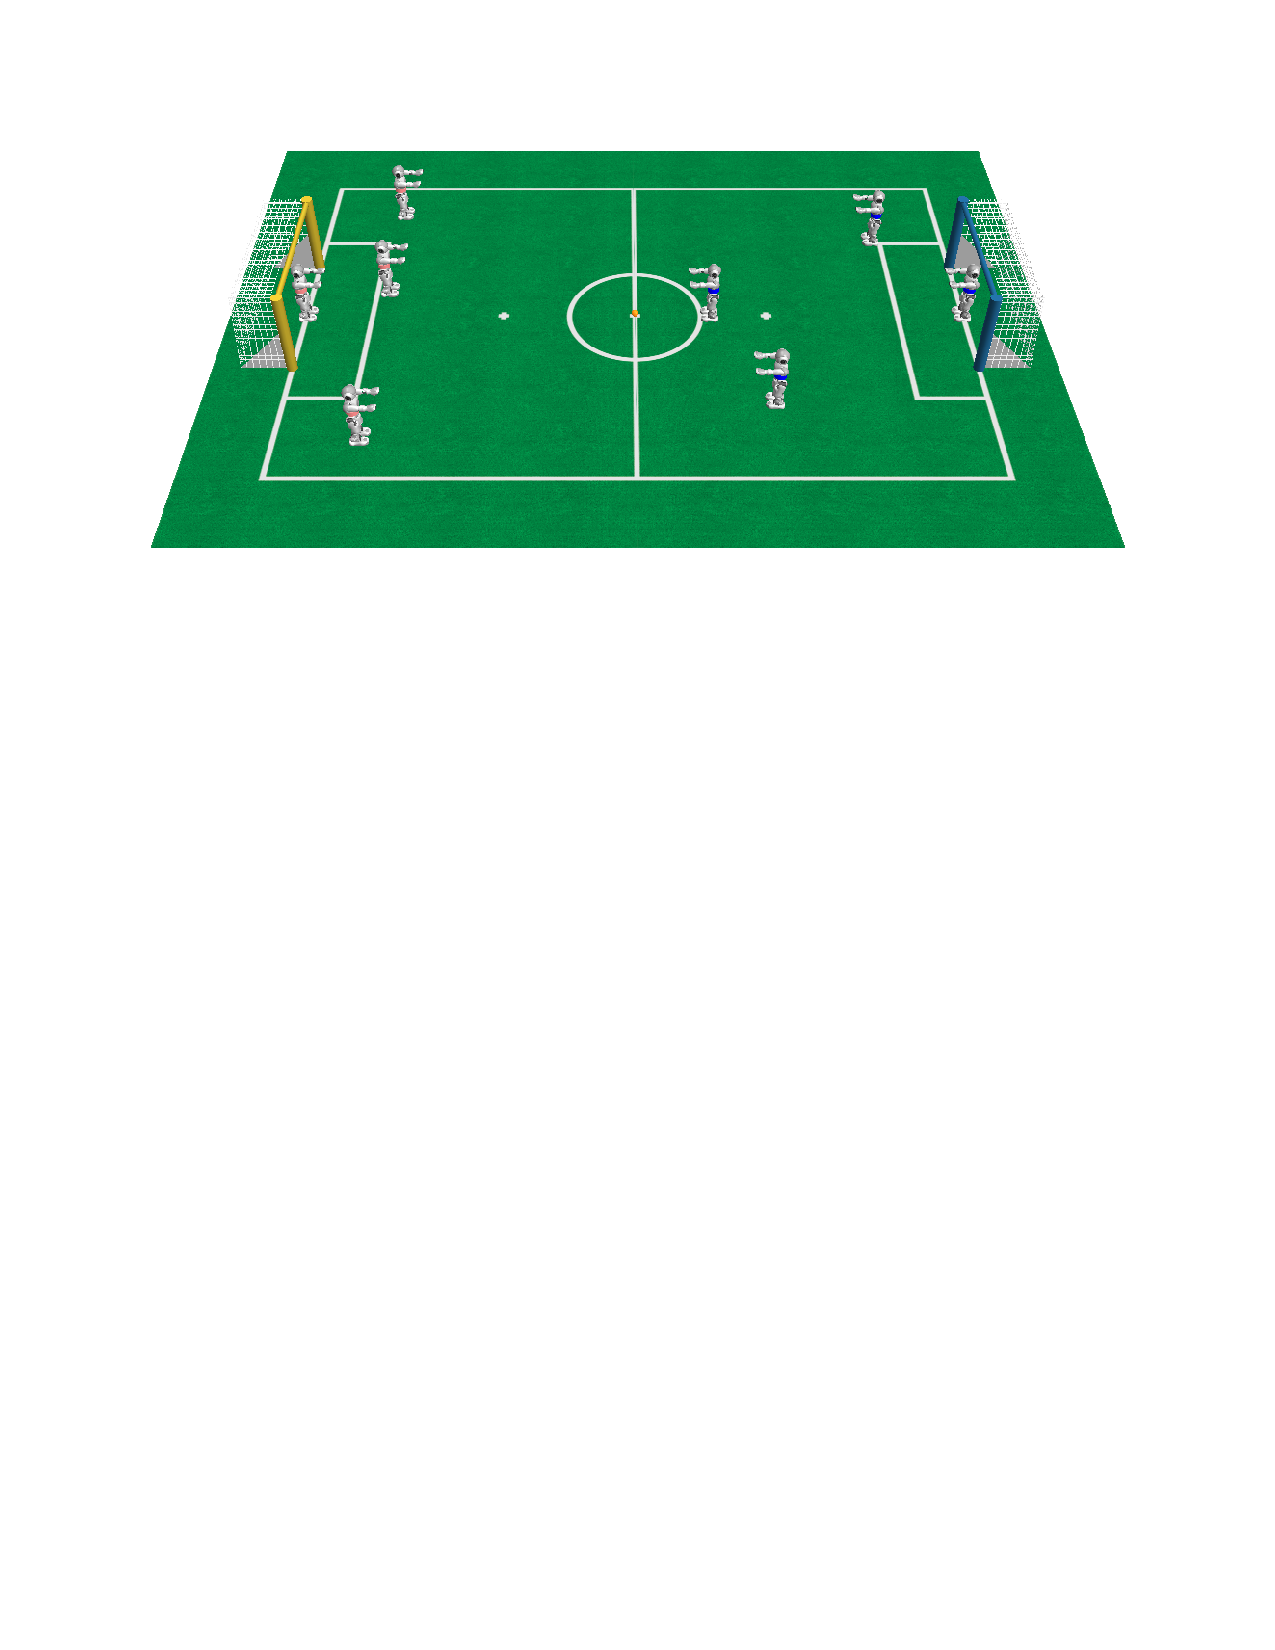
\includegraphics[width=0.8\textwidth]{../Drawings/robocup/NaoField.pdf}
    \caption{The standard setup for a game of football before kick-off \cite{Rules}}
    \label{fig:naofield}
\end{figure}

The robots can communicate with one another using a wireless network access point but are limited to a bandwidth of $500 Kbps$. Robots can commit fouls on one another and, for certain fouls, a robot is subject to a \textit{Standard Removal Penalty} \cite{Rules}. In this scenario, the robot is removed from the field for $30$ seconds, facing away from the field of play. It is then placed on the halfway line or the nearest possible alternative if there are obstacles such as robots currently situated on the halfway line. Robots can also be placed on their respective side of the field facing the opposition. The robot then has to localise itself after which it can continue to participate in the game.\\

\subsubsection{Nao Specifications}
\label{sec:naoSpecs}
The Nao robot to be used for the project will use the latest Nao head, Head $4.0$, that has been designed by Aldebaran Robotics \cite{NaoHead}. The specifications for the new Nao head are shown in \figref{fig:nao1} and \figref{fig:nao2} respectively. The head contains two cameras that are placed vertically above one another. These cameras provide a $640 \times 480$ resolution and operate at $30$ frames per second (fps). These cameras operate in the \textit{YUV422} colour space.\\

It is important to note that the Vertical field of view has been increased for each of the cameras respectively to $47.64^\circ$ which may make it possible to detect features on the ceiling above the Robocup field. In addition to this wider field of view, the robot has a yaw range of $-119.5^\circ$ to $119.5^\circ$ and a pitch range of $-38.5^\circ$ to $29.5^\circ$ as shown in \figref{fig:yawPitch}. This will aid the robot to detect features well above the Robocup field.\\ 

 \begin{figure}[ht!]
\begin{minipage}[b]{0.5\linewidth}
  \centering
    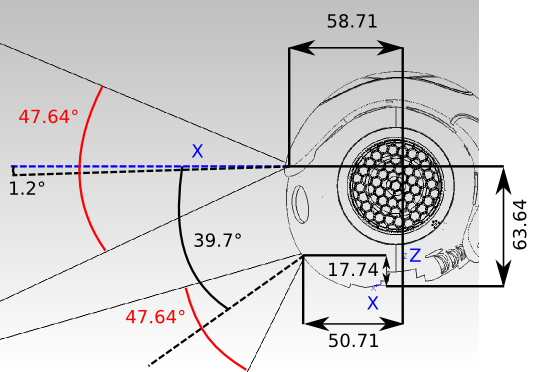
\includegraphics[width=0.6\textwidth]{../Drawings/naoHead/naoHead.jpg}
    \caption{A side view of the new Nao head \cite{NaoHead}} 
    \label{fig:nao1}
\end{minipage}
\begin{minipage}[b]{0.5\linewidth}
  \centering
    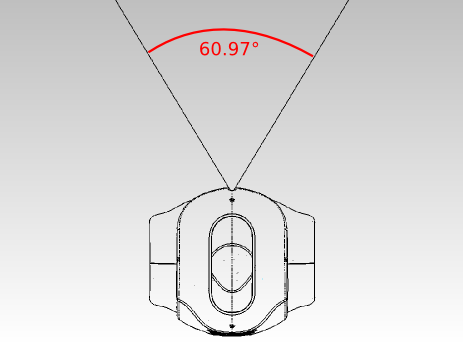
\includegraphics[width=0.6\textwidth]{../Drawings/naoHead/naoHead1.jpg}
    \caption{A top view of the new Nao head \cite{NaoHead}} 
    \label{fig:nao2}
\end{minipage}
\begin{minipage}[b]{0.5\linewidth}
  \centering
    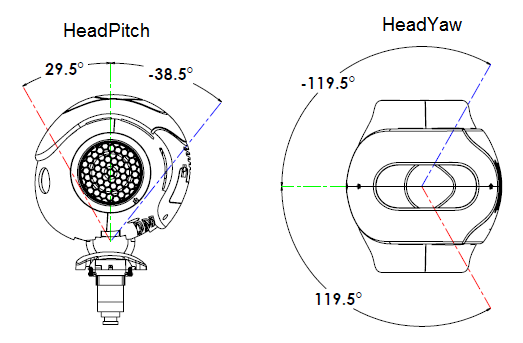
\includegraphics[width=1.0\textwidth]{../Drawings/naoHead/headyawpitch.png}
    \caption{The yaw and pitch of the Nao head \cite{NaoHead}} 
    \label{fig:yawPitch}
\end{minipage}
\end{figure}



\section{General Feature Extraction Techniques}
\label{sec:genFeatureExtract}
Throughout this paper, detector refers to the module of the feature extraction algorithm that is used to detect the interest points. Descriptor will refer to the module of the feature extraction algorithm that computes the descriptor for each interest point.\\

\subsection{2DSURF}
\label{sec:2dsurf}
The SURF feature extraction algorithm is based on approximating the Hessian matrix at every point in an image. The determinant of the Hessian is then computed at each point and is referred to as the blob response. This computation is performed over a number of different scales in scale-space as well as in image space in order to find local maxima. A non-maximal suppression is then performed and the local maxima that exist after this stage will be defined as interest points. Each interest point is represented by a descriptor of length $64$. Interest points in different images are then matched based on the Euclidean distance between their respective feature vectors. The smaller the distance, the more certain the match becomes. 

\subsubsection{Integral Images}
\label{sec:integralImages}
One of the big advantages in SURF over SIFT \cite{Lowe2004} is its computational efficiency. One of the important tools that are utilised in order to create this advantage in computation is called the Integral Image \cite{Bay2008}. An integral image computes the integral image value, $I_{int}(x,y)$ for pixel location $(x,y)$  as a sum of all pixel intensities found to the left and below the current pixel location until the origin. This is presented in \eqnref{eqn:integralImage}. The variable $I(x,y)$ is the individual pixel intensity at location $(x,y)$. Thus the value of each pixel can be interpreted as the area of the rectangle formed from the current pixel to the image origin. It is assumed that the image origin is in the top left corner of the image. \\

\begin{equation}
I_{int}(x,y) = \sum_{i=0}^{i \leq x}\sum_{j=0}^{j \leq y}I(x,y)
\label{eqn:integralImage}
\end{equation}

By computing the integral image, it is possible to reduce the calculation of any upright rectangular image to four operations. This is very useful when computing box filter convolutions that will be described in the sections to follow.\\

\subsubsection{Detector}
\label{2dsurfdetect}
The SURF detector is based on computing the determinant of the Hessian matrix. The Hessian matrix is a matrix of second order partial derivatives and, when calculated for an intensity image,  $I(x,y)$, it is of the form shown in \eqnref{eqn:hessian}.\\

\begin{equation}
Hessian = \left[ \begin{array}{cc} \frac{\partial I}{\partial x^2} & \frac{\partial I}{\partial x^2}\\
					    \frac{\partial I}{\partial x^2} & \frac{\partial I}{\partial x^2}\end{array} \right]
\label{eqn:hessian}
\end{equation}

The Hessian matrix is computed in order to identify local maxima and minima in the image. This is achieved by first computing the determinant, also know as the discriminant, of the Hessian matrix. The determinant of the Hessian is shown in \eqnref{eqn:determinant}. If the determinant of the Hessian is negative then a local extremum has not been identified. If the determinant is positive then a local extremum has been identified \cite{Evans2009}. \\

\begin{equation}
det\mid H \mid = \frac{\partial I}{\partial x^2} \frac{\partial I}{\partial y^2} - (\frac{\partial I}{\partial x \partial y})^2
\label{eqn:determinant}
\end{equation}

For a SURF detector, the Hessian is computed for a point $\textbf{x} = (x,y)$ in the Image $I$. The Hessian is computed over multiple scales, $\sigma$, and therefore the Hessian matrix at a point for a specific scale is represented as $H(\textbf{x}, \sigma)$ \cite{Lowe2004} and is defined as shown in \eqnref{eqn:hessianScale}.\\


\begin{equation}
H(\textbf{x}, \sigma) = \left[ \begin{array}{cc} L_{xx}(\textbf{x}, \sigma) & L_{xy}(\textbf{x}, \sigma)\\
					    L_{xy}(\textbf{x}, \sigma) & L_{yy}(\textbf{x}, \sigma)\end{array} \right]
\label{eqn:hessianScale}
\end{equation}

The variable $L_{xx}(\textbf{x}, \sigma)$ is analogous to the second order derivative, $ \frac{\partial I}{\partial x^2}$, detailed in \eqnref{eqn:hessian}. This second order derivative is computed in SURF detectors by convolving the image, at point $\textbf{x}$, with a particular kernel \cite{Evans2009}. The kernel in this instance is the second order Gaussian derivative, $\frac{\partial g(\sigma)}{\partial x^2)}$. \\

There are a number of reasons why Gaussians are used as the kernel in computing the second order derivatives. One of the main reasons is that it is possible to vary the amount of smoothing resulting from the convolution of the Gaussian with the image \cite{Evans2009}. This enables the calculation of the Hessian determinant at different scales which is used for non-maximal suppresion and identifying scale-invariant interest points.\\

The SURF implementation approximates Gaussian second order derivatives for the convolution stage by using box filters. Box filters are used to perform very fast convolutions. A box filter consists of positive and negative lobes. Each lobe is assigned a particular weighting. For example, in \figref{fig:boxFilters} \cite{Bay2008}, the white lobes are assigned a weighting of positive one, the black lobes are assigned a weighting of negative one and the gray lobes are assigned a weighting of 0. The box filters are created in the $x$, $y$ and $xy$ directions in order to compute the Hessian and subsequently its determinant. One of the key advantages to this approach is the computational cost. This is because it is possible to use a combination of integral images and box filters to perform the second order derivative computation very efficiently. It is also possible to increase the size of the box filters at no additional computational cost \cite{Bay2008}.\\

\begin{figure}[h!] 
  \centering
    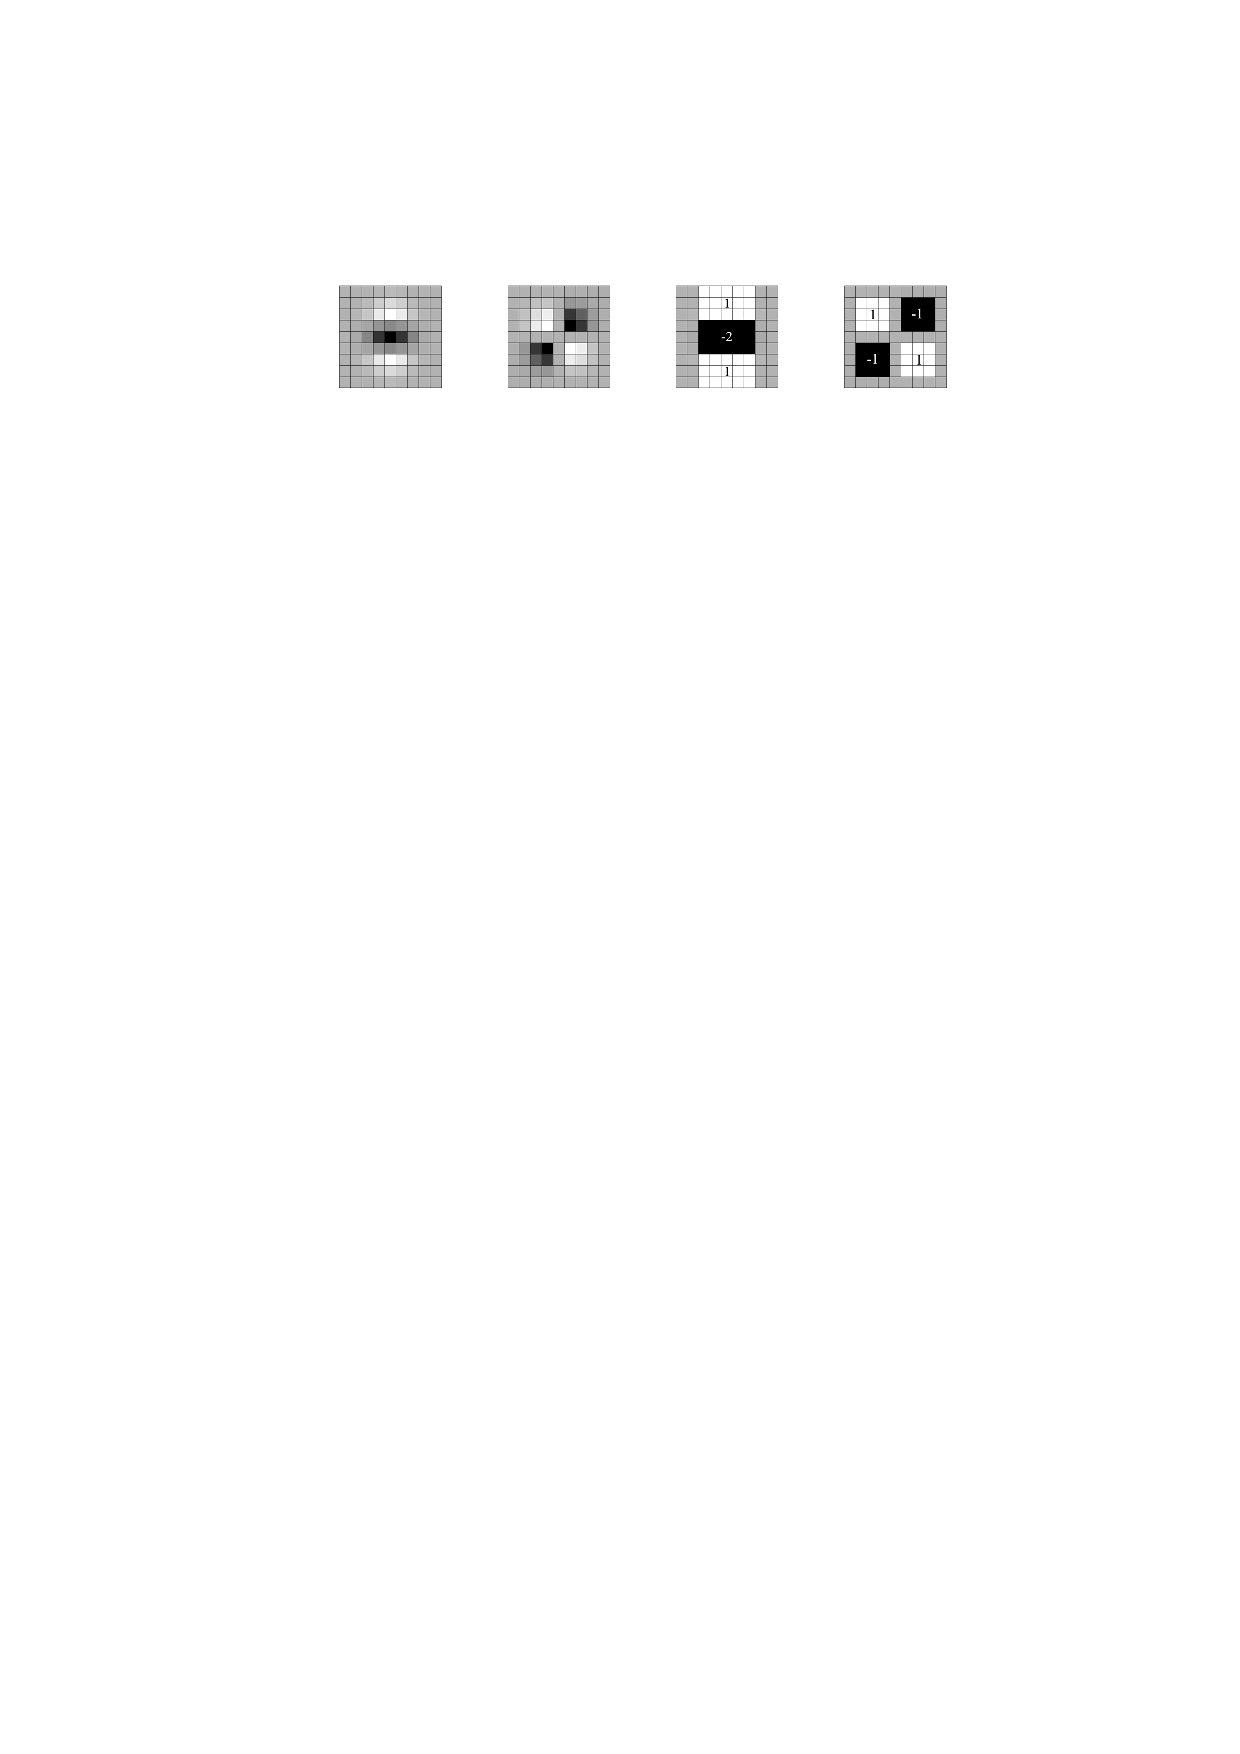
\includegraphics[width=0.8\textwidth]{../Drawings/methods/SURF2D_BoxFilters.pdf}
    \caption{The Box filters used to perform the 2D convolutions}
    \label{fig:boxFilters}
\end{figure}

Therefore, utilising box filters, the determinant of the Hessian is computed as shown in \eqnref{eqn:approxHessian}. The variables $D_{xx}$, $D_{xy}$ and $D_{yy}$ represent the box filter convolutions in the $x$, $xy$ and $y$ directions respectively at a point $\textbf{x} = (x,y)$ in the image $I$.\\ 

\begin{equation}
det \mid H_{approx} (x,y) \mid = D_{xx}D_{yy} - (0.9 D_{xy}^2)
\label{eqn:approxHessian}
\end{equation}

The determinant of the Hessian at a point $\textbf{x} = (x,y)$ in the image $I$ is referred to as the blob response at a scale $\sigma$ \cite{Bay2008}. The blob response is computed at every location in the image in order to create a blob response map. A blob response map exists for every considered scale and these maps are used to detect local maxima in the images.\\

The different scales collectively define the scale space. The scale space can be seen as a function that is used to find extrema across a set of pre-defined scales. A set of scales is important as interest points need to be found across a number of scales in order to verify that the point is indeed an interest point. It also ensures that the point can be detected at different scales (I.e. points of view).\\

In the SIFT method \cite{Lowe2004}, in order to construct the scale space, an image is convolved with a Gaussian kernel. The image is then sub-sampled and re-convolved with the same kernel to create a new scale. In the SURF method, as mentioned previously, the box filter size can be increased at no computational cost due the use of integral images. Thus it makes sense to construct the scale space by convolving the image with the box filters, but instead of sub-sampling the image, the box filters can be increased in size and convolved with the same image at very little computational cost. This creates a very efficient `inverted' scale space pyramid as shown in \figref{fig:scaleSpace} \cite{Evans2009}. The higher the position in the pyramid, the larger the scale and vice versa. \\

\begin{figure}[h!] 
  \centering
    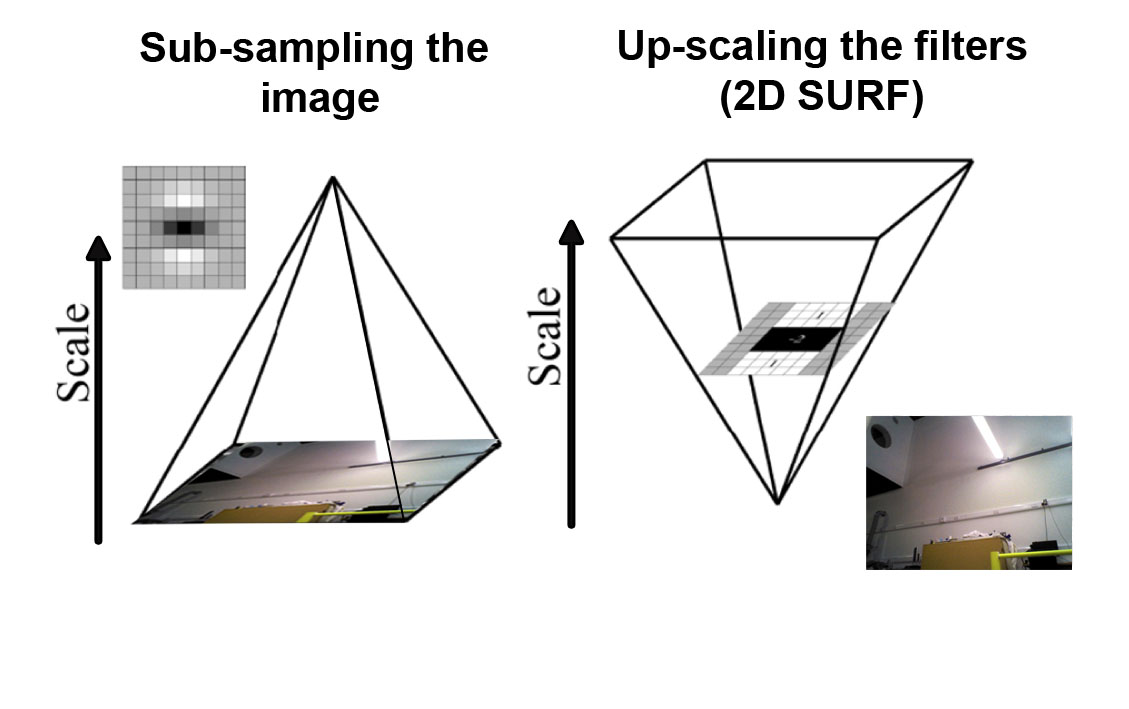
\includegraphics[width=0.8\textwidth]{../Drawings/methods/SURF2D_Image_pyramid.jpg}
    \caption{The up-scaling of the filters is used in 2D SURF rather than the down-scaling of the image}
    \label{fig:scaleSpace}
\end{figure}

The scale space is divided into octaves. An octave consists of a set of blob response maps each resulting from a convolution of the image with a box filter of a specific size. The blob response map corresponding to the lowest level (I.e. smallest scale) of the scale space is constructed using a $9 \times 9$ box filter. This corresponds to a scale value of $1.2$. As the size of the filters used for convolution increase, so too does the scale. During the convolution procedure, the filter is centered on each $(x,y)$ location in the image and each lobe in the filter has a specific width represented by $l_0$. In order to increase the size of the filter (I.e. move up a level in scale space), the filter lobe width, $l_0$, is increased by $2$ pixels. This ensures that the center pixel is still found in the center of the filter. Thus, the first filter is $9 \times 9$ and the next successive filter is $15 \times 15$. \\

The number of octaves used to find interest points depend on the size of the image. Usually, three to four octaves are used. The first octave uses box filters of size $9 \times 9$, $15 \times 15$, $21 \times 21$ and $27 \times 27$ to convolve with the current image.  For each subsequent octave, the filter size increase is doubled. Therefore, for example, the second octave will have filter sizes of $15 \times 15$, $27 \times 27$, $39 \times 39$ and $51 \times 51$ respectively. This corresponds to a filter increase of $12$ pixels. The next octave will have an increase of $24$ pixels and so on \cite{Bay2008}. \\

As mentioned previously, the convolution of the box filters of various sizes produces blob response maps at various scales. The next step involves using the blob response maps to detect interest points at these different scales. The first step in detecting interest points is removing pixels whose blob responses are below a certain threshold. Once the relevant pixels have been thresholded,  a non-maximal suppression is performed in a $3 \times 3 \times 3$ neighborhood surrounding the current pixel. Thus for each octave and each scale within the octave, each pixel is compared to its $26$ neighbors \cite{Evans2009}. This includes its $8$ adjacent neighbors in image space as well as its $9$ neighbors in the scale above and scale below the current image space respectively as shown in \figref{fig:imageSpace} \cite{Lowe2004}. It should be noted that the largest scale and smallest scale for each octave have no scale space layers above or below respectively. Therefore these blob response maps are only used for comparison for the internal scale-space layers. \\

\begin{figure}[h!] 
  \centering
    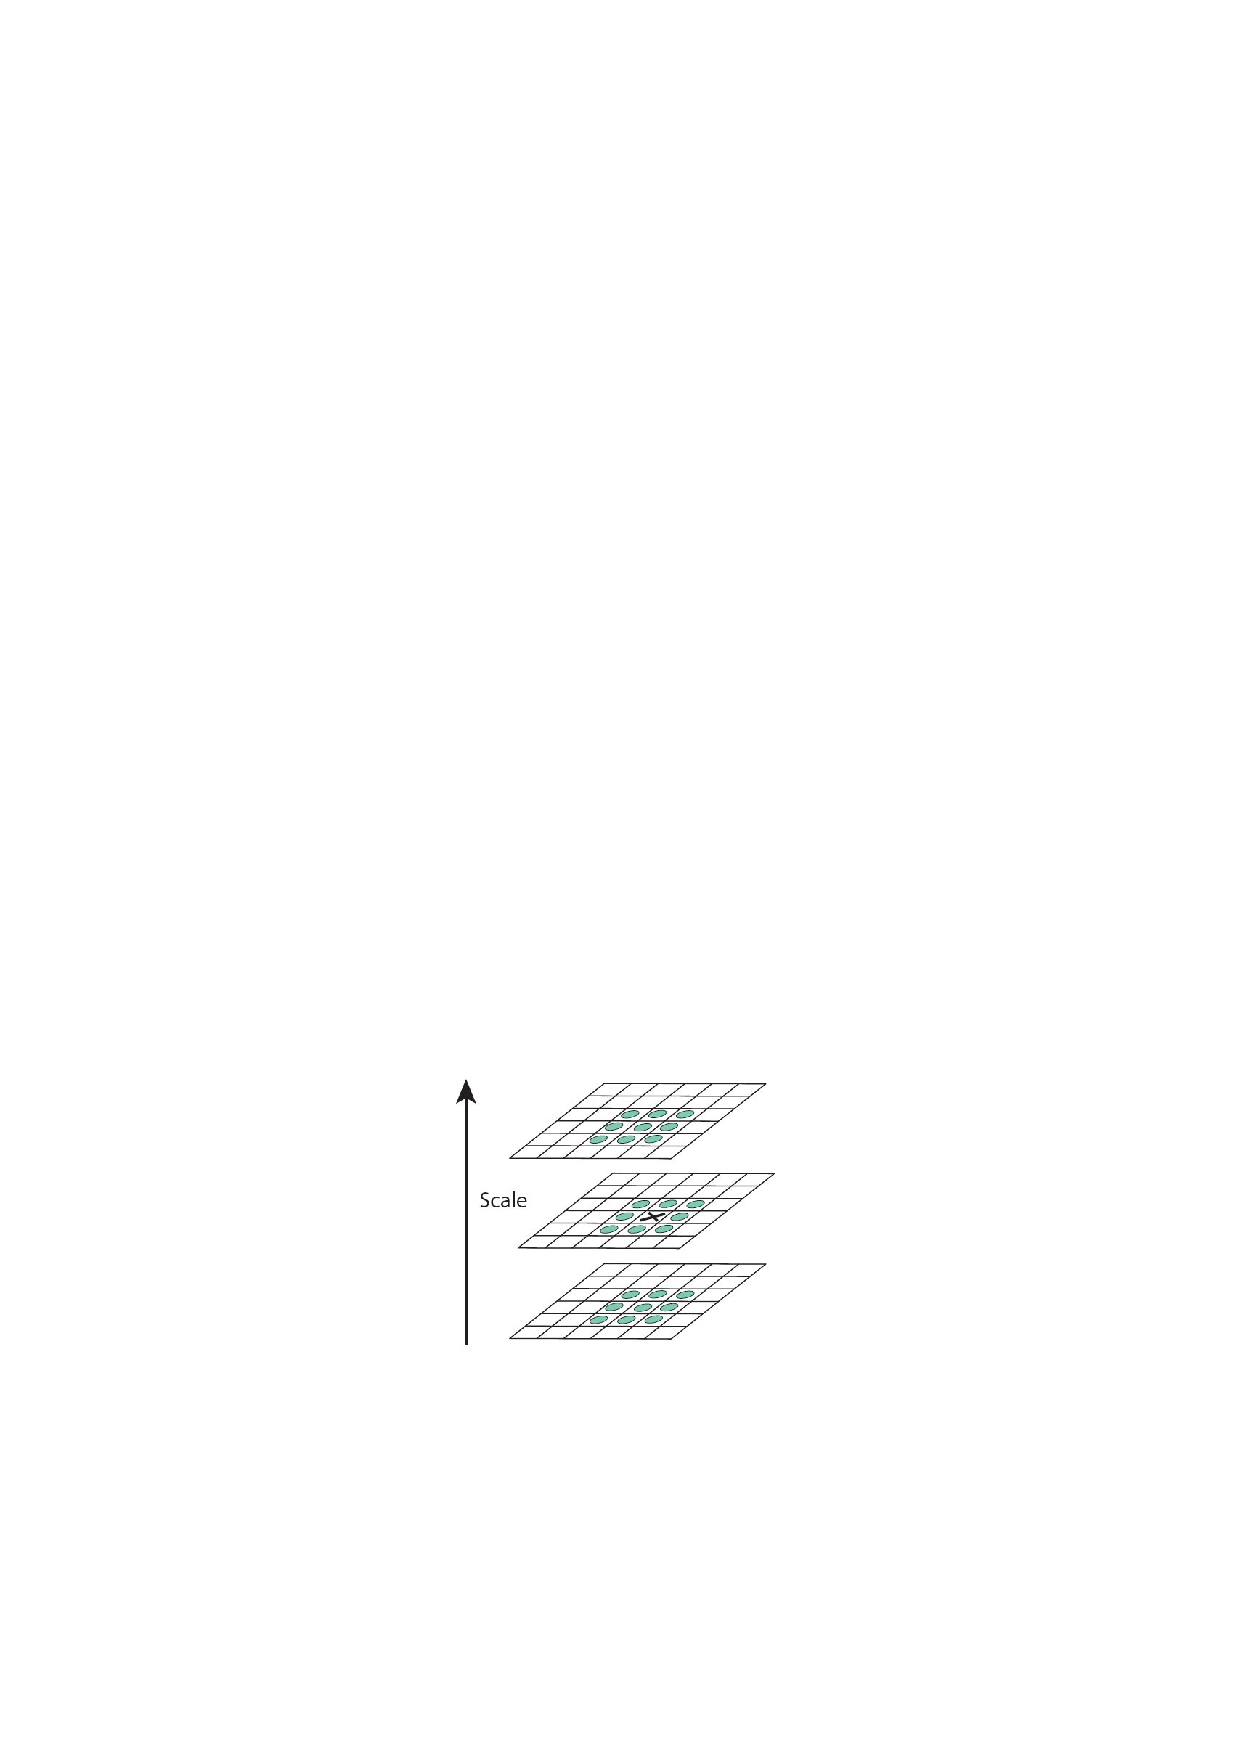
\includegraphics[width=0.5\textwidth]{../Drawings/methods/SURF2D_Nonmaximal_suppression.pdf}
    \caption{The non-maximal suppression performed on each point and its $26$ surrounding neighbors.}
    \label{fig:imageSpace}
\end{figure}

If the pixel is not suppressed, then its image space and scale space locations are calculated to sub-pixel accuracy using a linear interpolation procedure \cite{Evans2009}. The pixel becomes an interest point and its descriptor then needs to be determined.\\

%The interpolation procedure TO DO Maybe...

\subsubsection{Descriptor}
\label{sec:2dsurfdescribe}
The SURF descriptor is a $64$ length vector that contains information about the intensity content of the neighborhood surrounding the interest point. In developing the descriptor, a number of important steps need to be implemented. The first step is creating a reproducable orientation for the interest point \cite{Bay2008}. If the interest point was detected at a scale, $\sigma$, then Haar Wavelets of size $4\sigma$ are used to calculate Haar Wavelet Responses (HWRs) for all pixels within a circular radius of $6\sigma$ from the detected interest point.  Haar Wavelets are simple filters that are used in SURF to calculate gradients in the $x$ and $y$ directions respectively. Examples of these wavelets are shown in \figref{fig:haar} \cite{Evans2009}. Once the HWRs have been calculated, they are then weighted by a Gaussian whose mean is centered on the interest point. This means that the pixels found further away from the interest point have a smaller influence on the reproducible interest point orientation.\\


\begin{figure}[h!] 
  \centering
    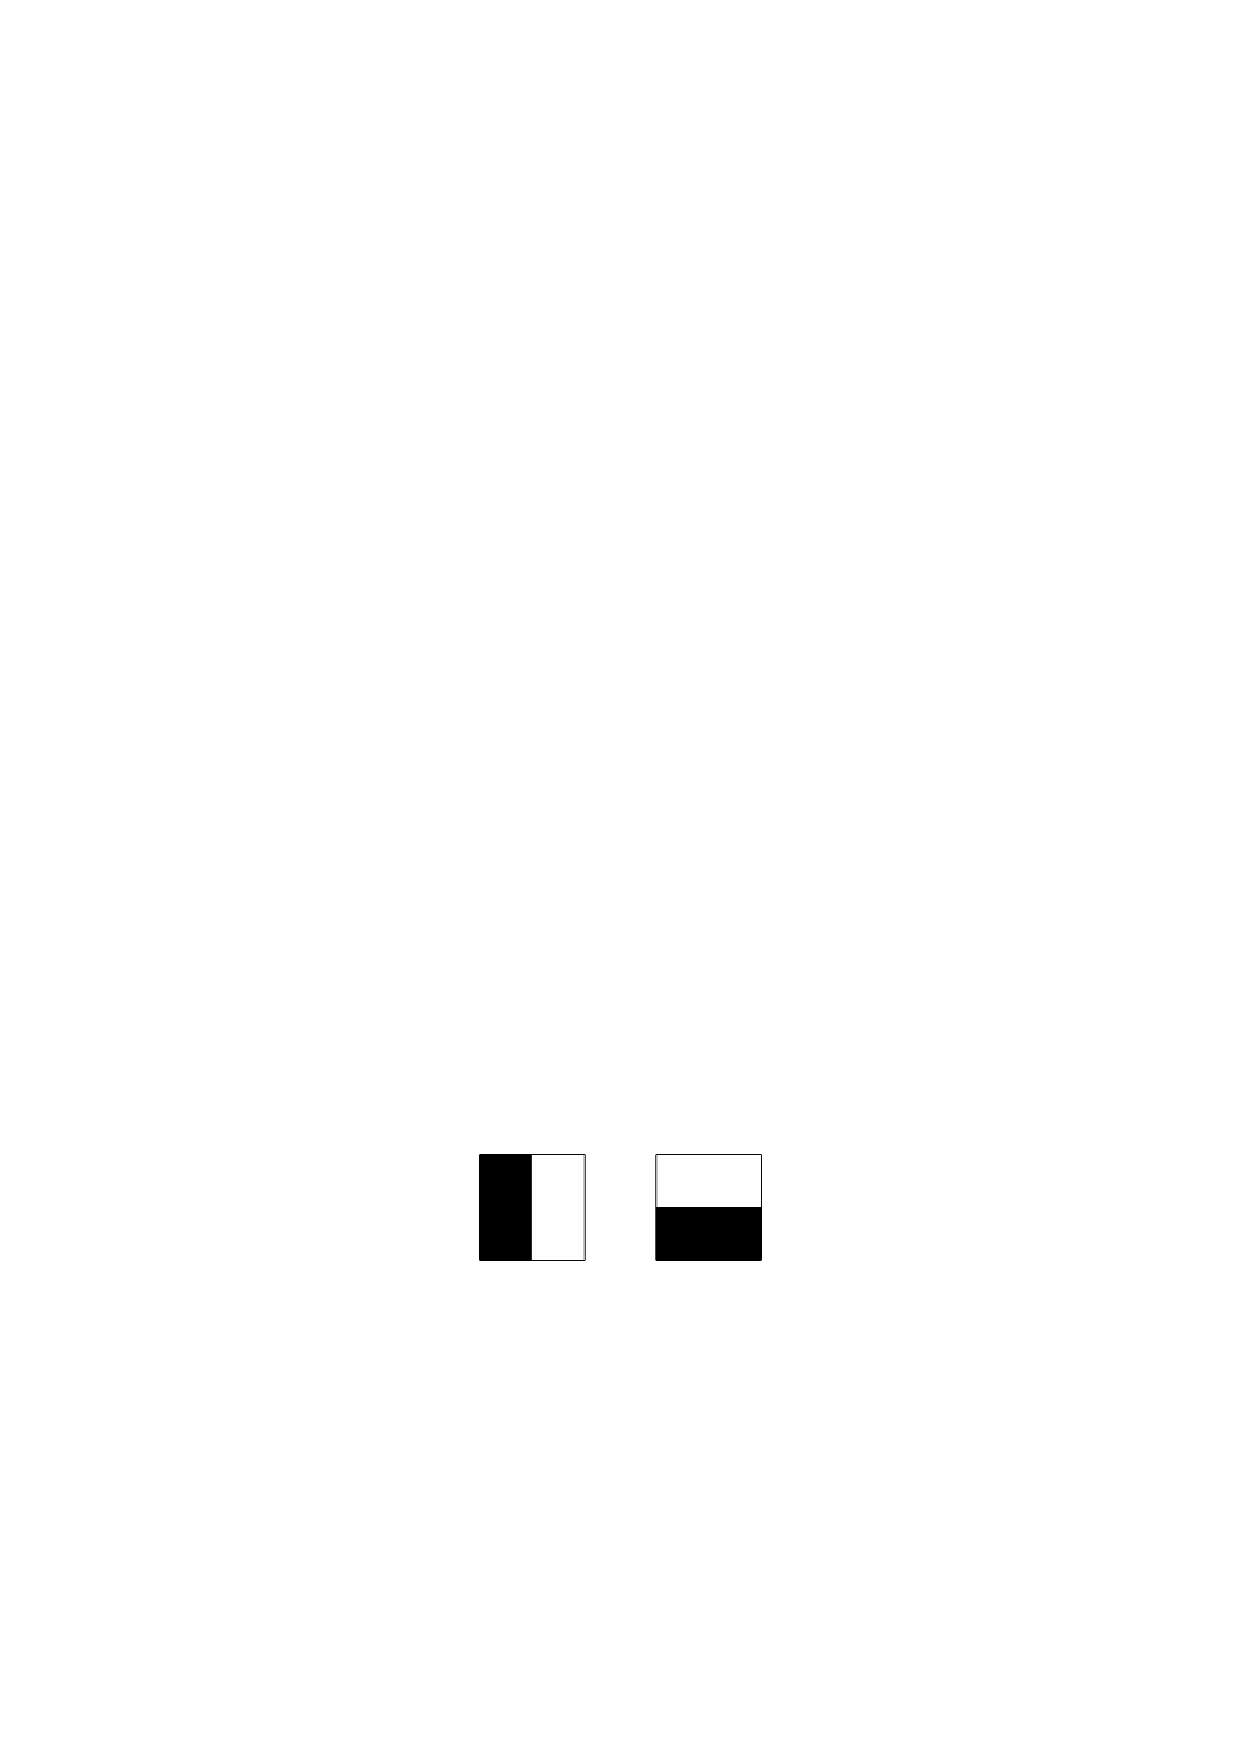
\includegraphics[width=0.5\textwidth]{../Drawings/methods/SURF2D_HaarWavelets.pdf}
    \caption{Haar Wavelets used to calculate the Haar Wavelet Responses. The left Haar Wavelet calculates the responses in the $x$ direction and the right one calculates the Haar Wavelets in the $y$ direction}
    \label{fig:haar}
\end{figure}

In order to find the reproducible orientation, a circular segment of width $\frac{\pi}{3}$ is rotated around the interest point and the HWRs in the $x$ and $y$ directions, within this circular segment, are calculated to yield a vector for that particular circular segment as shown in \figref{fig:circularSegment} \cite{Evans2009}. The longest vector resulting from the rotation of this circular segment around the interest point is assigned to the interest point as the reproducible orientation.\\

\begin{figure}[h!] 
  \centering
    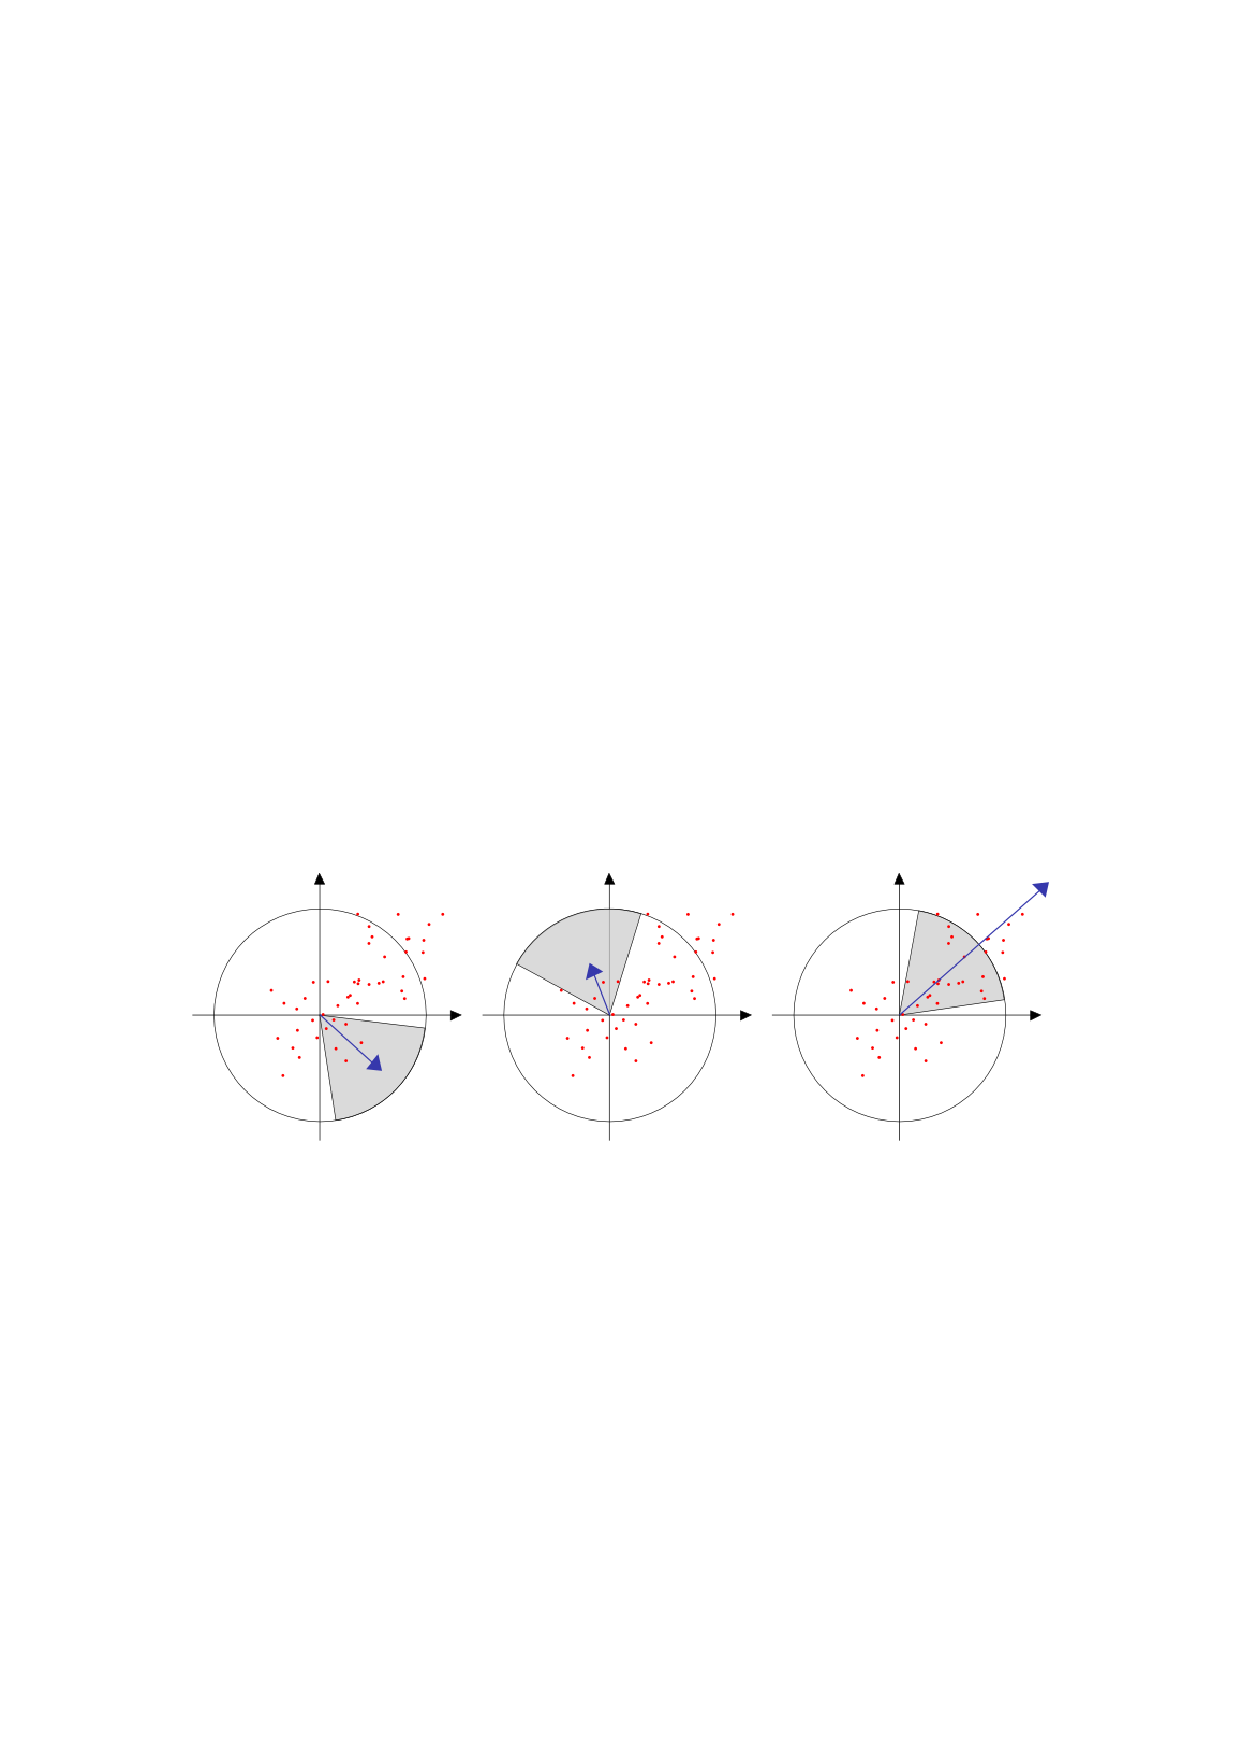
\includegraphics[width=1.0\textwidth]{../Drawings/methods/SURF2D_orientation_assignment.pdf}
    \caption{The $\frac{\pi}{3}$ circular segment calculating the Haar Wavelet Responses for a particular interest point. Here, the right-most figure contains the largest vector and the interest point is therefore assigned the orientation of this vector.}
    \label{fig:circularSegment}
\end{figure}

Once the orientation of the interest point has been determined, a square window of size $20\sigma$ is centered around the interest point and is oriented in the direction of the reproducible orientation of that interest point. This square region is then split into $16$ sub-regions of equal size. In each sub-region, HWRs in the $x$ and $y$ directions are then computed for $5 \times 5$ regularly spaced sample points. It is important to note that the $x$ and $y$ directions are relative to the reproducible orientation axes as shown in \figref{fig:reproducibleAxes} \cite{Evans2009}. The HWRs for these $25$ sample points are then summed together to yield the descriptor for the subregion as shown in \eqnref{eqn:descriptorSub}. Since there are $16$ of these sub-regions, a $64$ length descriptor is created.\\

\begin{figure}[h!] 
  \centering
    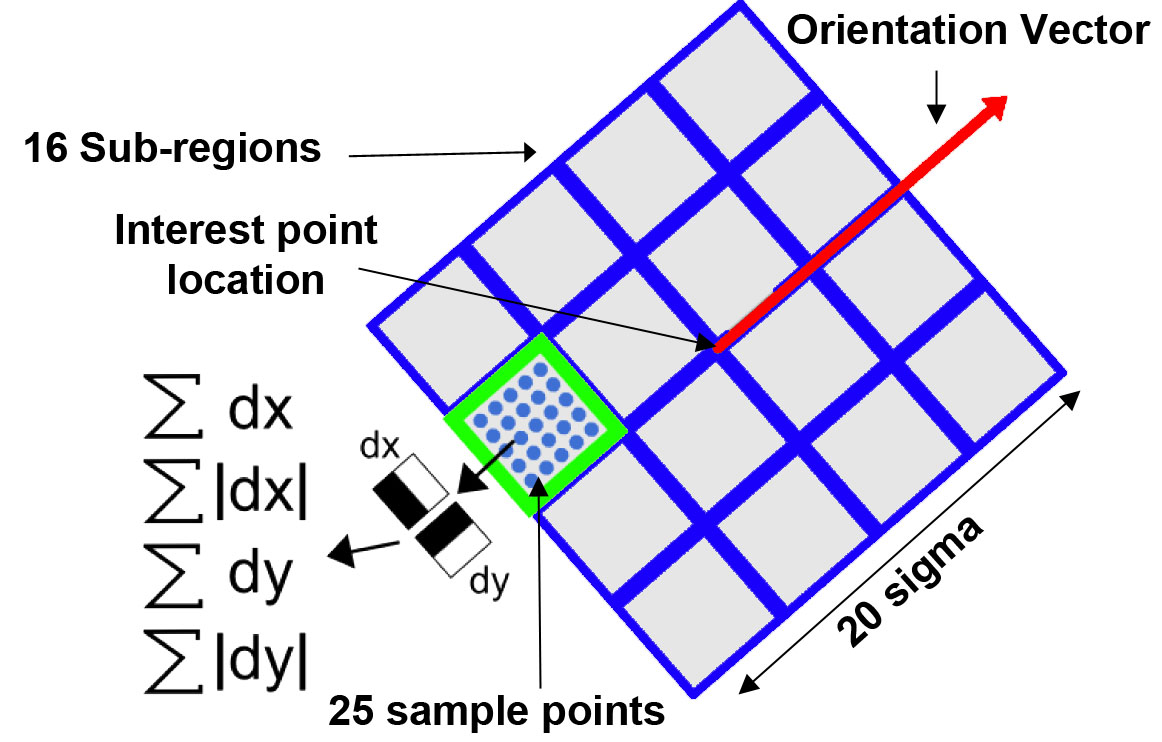
\includegraphics[width=0.5\textwidth]{../Drawings/methods/SURF2D_Descriptor.jpg}
    \caption{The square window centered on the interest point and aligned with the orientation vector.}
    \label{fig:reproducibleAxes}
\end{figure}

\begin{equation}
descriptor_{sub} = [\Sigma d_x, \Sigma d_y,  \Sigma \mid d_x \mid , \Sigma \mid d_y \mid] 
\label{eqn:descriptorSub}
\end{equation} 



\subsection{BRISK}
\label{sec:brisk}
A new method has been developed that, in a variety of domains yields performance that betters SURF by an order of magnitude. This method is called Binary Robust Invariant Scalable Keypoints (BRISK) \cite{Leutenegger2011}. This method utilises a technique called Adapative and Generic Corner Detection Based on the Accelerated Segment Test (AGAST) in order to compute a score for a pixel in location $(x,y)$ in image $I$ \cite{Mair2010}. AGAST is largely base on the Features from Accelerated Segment Test (FAST) \cite{Rosten2006} method but incorporates some improvements such as adaptive tree switching which will be briefly discussed. Using this score, interest points are defined. A binary feature descriptor of length $512$ is then generated for each interest point as a result of some simple brightness comparison tests. Interest points are then matched in different images by computing the Hamming distance between the feature descriptors. \\

\subsubsection{FAST Score}
\label{sec:fastScore}

The FAST score, denoted as $s$, is the first criterion that is used in BRISK in order to identify interest points \cite{Rosten2006}. The FAST score is computed by initially choosing a set of $16$ pixels that form a circle centered on the current pixel $p$. $p$ is the potential interest point that is being evaluated, as shown in \figref{fig:fastScore} \cite{Rosten2006}. The circle has a Bresenham radius of $3.4$ pixels \cite{Mair2010}. In order for the pixel $p$ to be considered an interest point, there has to be a set of $n$ (in this case $9$) contiguous pixels from the circle of $16$ pixels that are brighter than the current pixel intensity, $I_p$, plus some threshold $t$, or are darker than $I_p - t$. A larger value of $t$ will reduce the amount of interest points that will be detected. However, these detected points will be strong, salient interest points. \\

\begin{figure}[h!] 
  \centering
    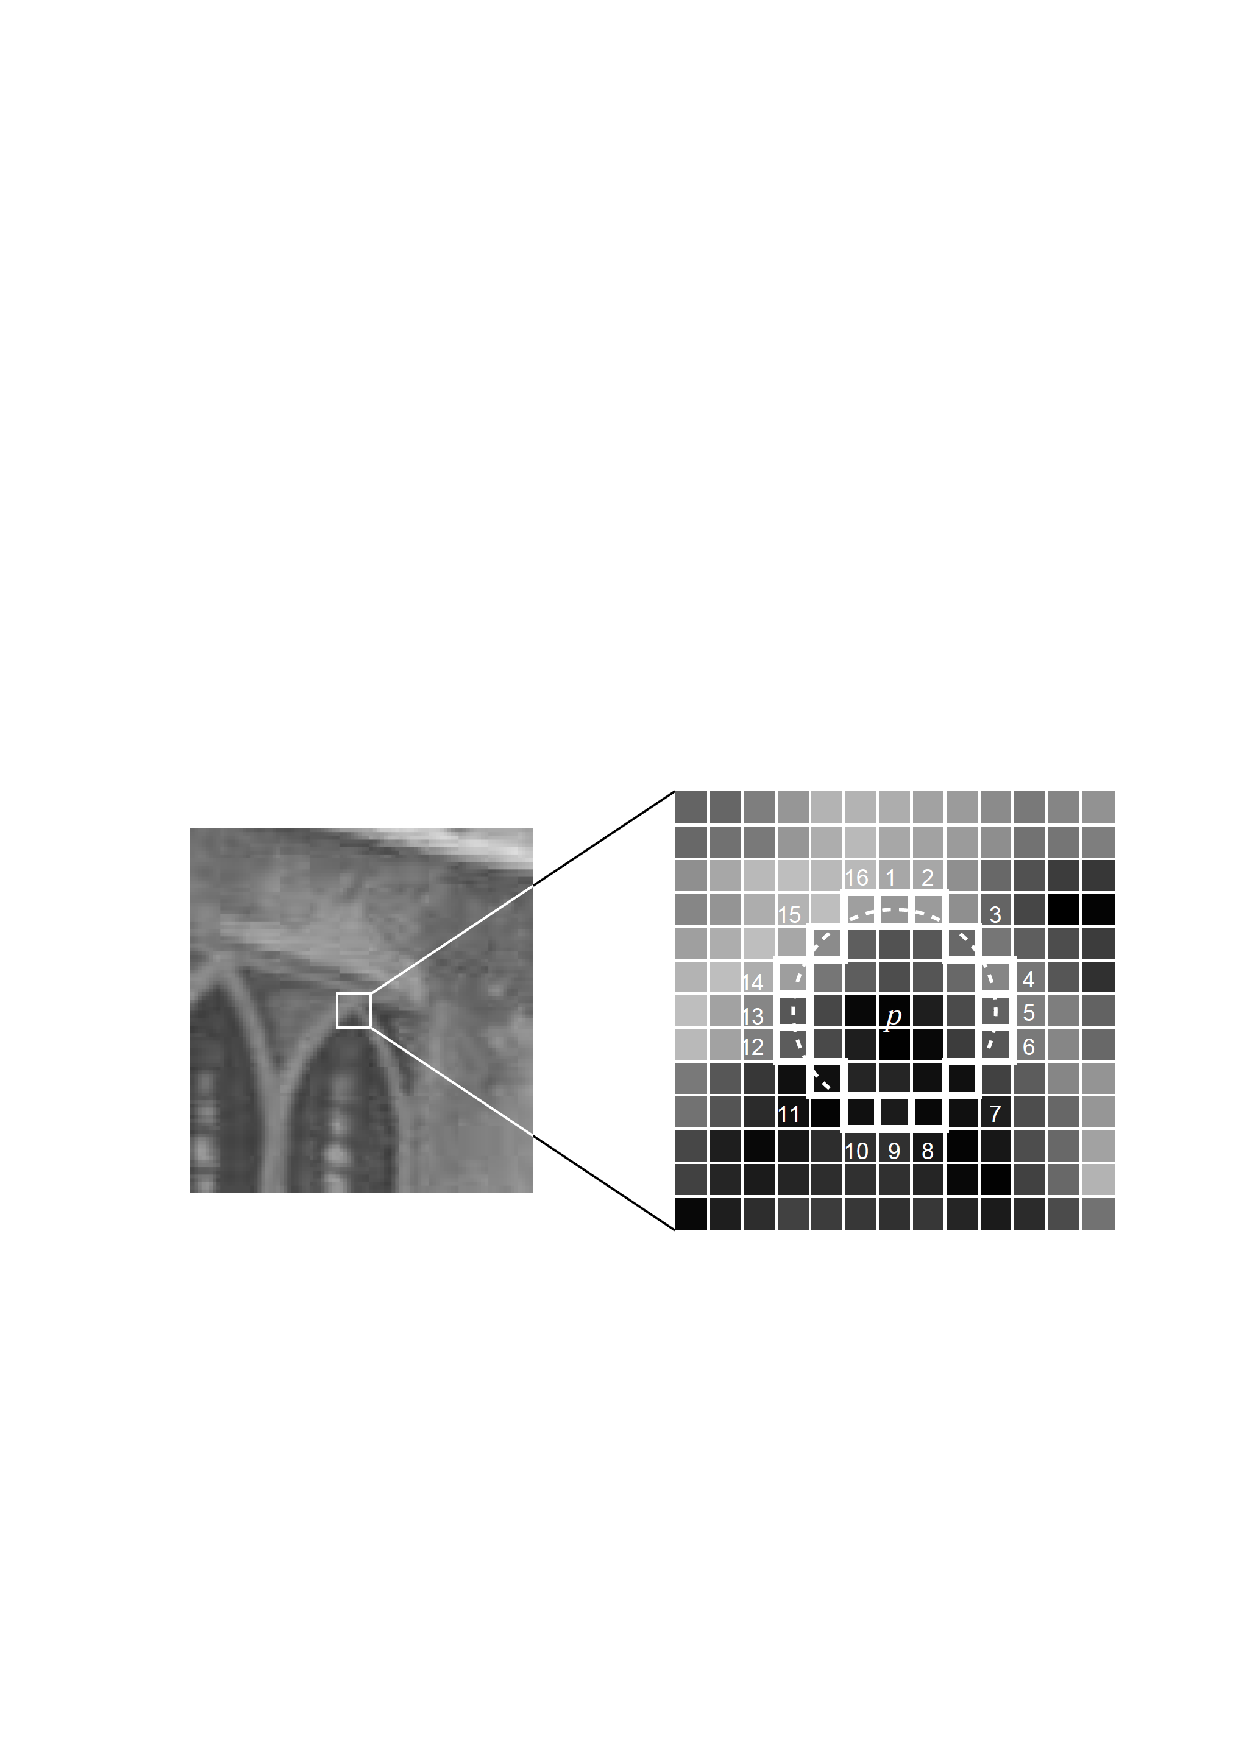
\includegraphics[width=0.8\textwidth]{../Drawings/methods/FASTScoreCalculation.pdf}
    \caption{The calculation of the FAST score for BRISK}
    \label{fig:fastScore}
\end{figure}

The FAST score is computed as the sum of the absolute difference between the circle of pixels and the central pixel. More formally it is expressed as shown in \eqnref{eqn:fastScore}. The variable $I_p$ is the intensity of the central pixel $p$. $I_{p \rightarrow x}$ is the intensity of the pixel at location $x$ on the circle of pixels relative to $p$. $S_{dark}$ refers to all the pixels that are darker than $I_p - t$, whereas $S_{bright}$ refers to all the pixels on the circle that are brighter than $I_p + t$. Taking the maximum of these two quantities yields the FAST score that is used for comparison in determining whether or not the pixel $p$ is an interest point.\\

\begin{equation}
V = max(\sum_{x \epsilon S_{bright}} \mid I_{p \rightarrow x} - I_p \mid - t, \sum_{x \epsilon S_{dark}} \mid I_p - I_{p \rightarrow x} \mid - t)
\label{eqn:fastScore}
\end{equation}

It is important to consider the order in which the points on the circle surrounding the potential interest point are evaluated, for computational efficiency. One method is to evaluate pixels $1, 5, 9 $ and $13$ corresponding to the compass directions \cite{Rosten2006}. At least three of these pixels need to be brighter or darker than the central pixel $p$ plus the chosen threshold in order for the central pixel to be evaluated further. If this is not the case, then the pixel $p$ is discarded as it cannot have $9$ contiguous pixels as mentioned previously and is therefore not an interest point. If at least three of the above-mentioned pixels fulfil the criteria, then the Accelerated Segment Test (AST) is applied to the circle of pixels in order to determine whether or not the central pixel is indeed an interest point. There are a different ways of applying the AST in order to determine whether or not a point is an interest point. Both FAST and AGAST use decision trees to search the circle of pixels in a specific order so as to maximise the efficiency with which each potential interest point is evaluated. The techniques differ in terms of the order in which the $16$ circle pixels are evaluated. In addition, AGAST has an adaptive tree switching technique which enables the method to switch to different decision trees that are optimised for a particular area of an image. This has an effect on computational efficiency and how well the methods generalise to different domains.   \\

FAST performs the AST by first learning a \textit{ternary} tree which has possible pixel states of \textit{brighter}, \textit{darker} or \textit{similar}. In building the tree, at each step, all remaining pixels are asked the question whether or not they are \textit{brighter} or \textit{darker} than the central pixel. The pixel with the highest information gain is chosen as the next branch in the tree. Each pixel can have one of four possible states, namely unknown (u), darker(d), brighter(b) or similar(s). Since $16$ pixels are being evaluated in the circle surrounding the central pixel and each of these pixels have four possible states, there are a total of $4^{16}$ possible configurations. \\

AGAST performs a more efficient and generic AST than that of FAST. One improvement in AGAST's method is that it has a richer configuration space. In addition, a \textit{binary} tree is constructed rather than a \textit{ternary} tree. \textbf{TO DO}\\

\subsubsection{Detector}
\label{briskDetect}
BRISK's scale space has a different structure to that of SURF. In this case, the scale space consist of \textit{n} octaves \textit{$c_i$} and \textit{n} intra-octaves \textit{$d_i$} \cite{Leutenegger2011}. The typical number of octaves chosen for BRISK is $n=4$. The intra-octaves are placed between the octaves. A typical ordering would be $c_0, d_0, c_1, d_1, c_2...$. In order to create the octaves, the image is progressively half-sampled by a factor of two. The first octave corresponding to the original image is called $c_0$ and the first intra-octave $d_0$ is generated by down-sampling the original image by a factor of $1.5$. Thereafter, the image is half-sampled by a factor of two. This creates an image pyramid where the lowest layer is the original image and the higher layers are down-sampled versions of the original image.\\

In BRISK, the FAST score $s$ is computed for each pixel $p$, for each octave and intra-octave respectively \cite{Leutenegger2011}. The same threshold $t$ is used throughout. A non-maximal suppression is then performed on each pixel in every octave and intra-octave respectively. In order to determine whether or not the pixel is indeed an interest point, the pixel $p$ firstly needs to be a maxima (in terms of its FAST score) compared to its $8$ adjacent neighbors in image space. The pixel's FAST score is then compared to the layer above and layer below in the image pyramid. Its FAST score has to be a maxima relative to these values as well. In the case of the original image $c_0$, no layer below this layer exists. To account for this problem, only the layer above $c_0$ is compared.\\

Once a pixel with a maximum score has been detected, a sub-pixel refinement is applied to the maximum by fitting a 2D quadratic function in the least squares sense to a $3 \times 3$ score patch surrounding the detected maximum \cite{Leutenegger2011}. A sub-pixel refinement is also applied to $3 \times 3$ patches in the layers directly above and below the detected maximum in order generate three local maxima. This procedure is followed by a continuous scale refinement in order to determine the true scale of the detected interest point. A 1D parabola is fitted to these three local maxima along the scale axis as shown in \figref{fig:1dparabola} \cite{Leutenegger2011} and the maximum of this parabola determines the true score and scale of the detected corner. Once the scale has been found, the image coordinates need to be re-interpolated to account for the true scale as the scale may not necessarily lie directly on an octave or intra-octave respectively. This creates a scale invariant interest point.\\

\begin{figure}[h!] 
  \centering
    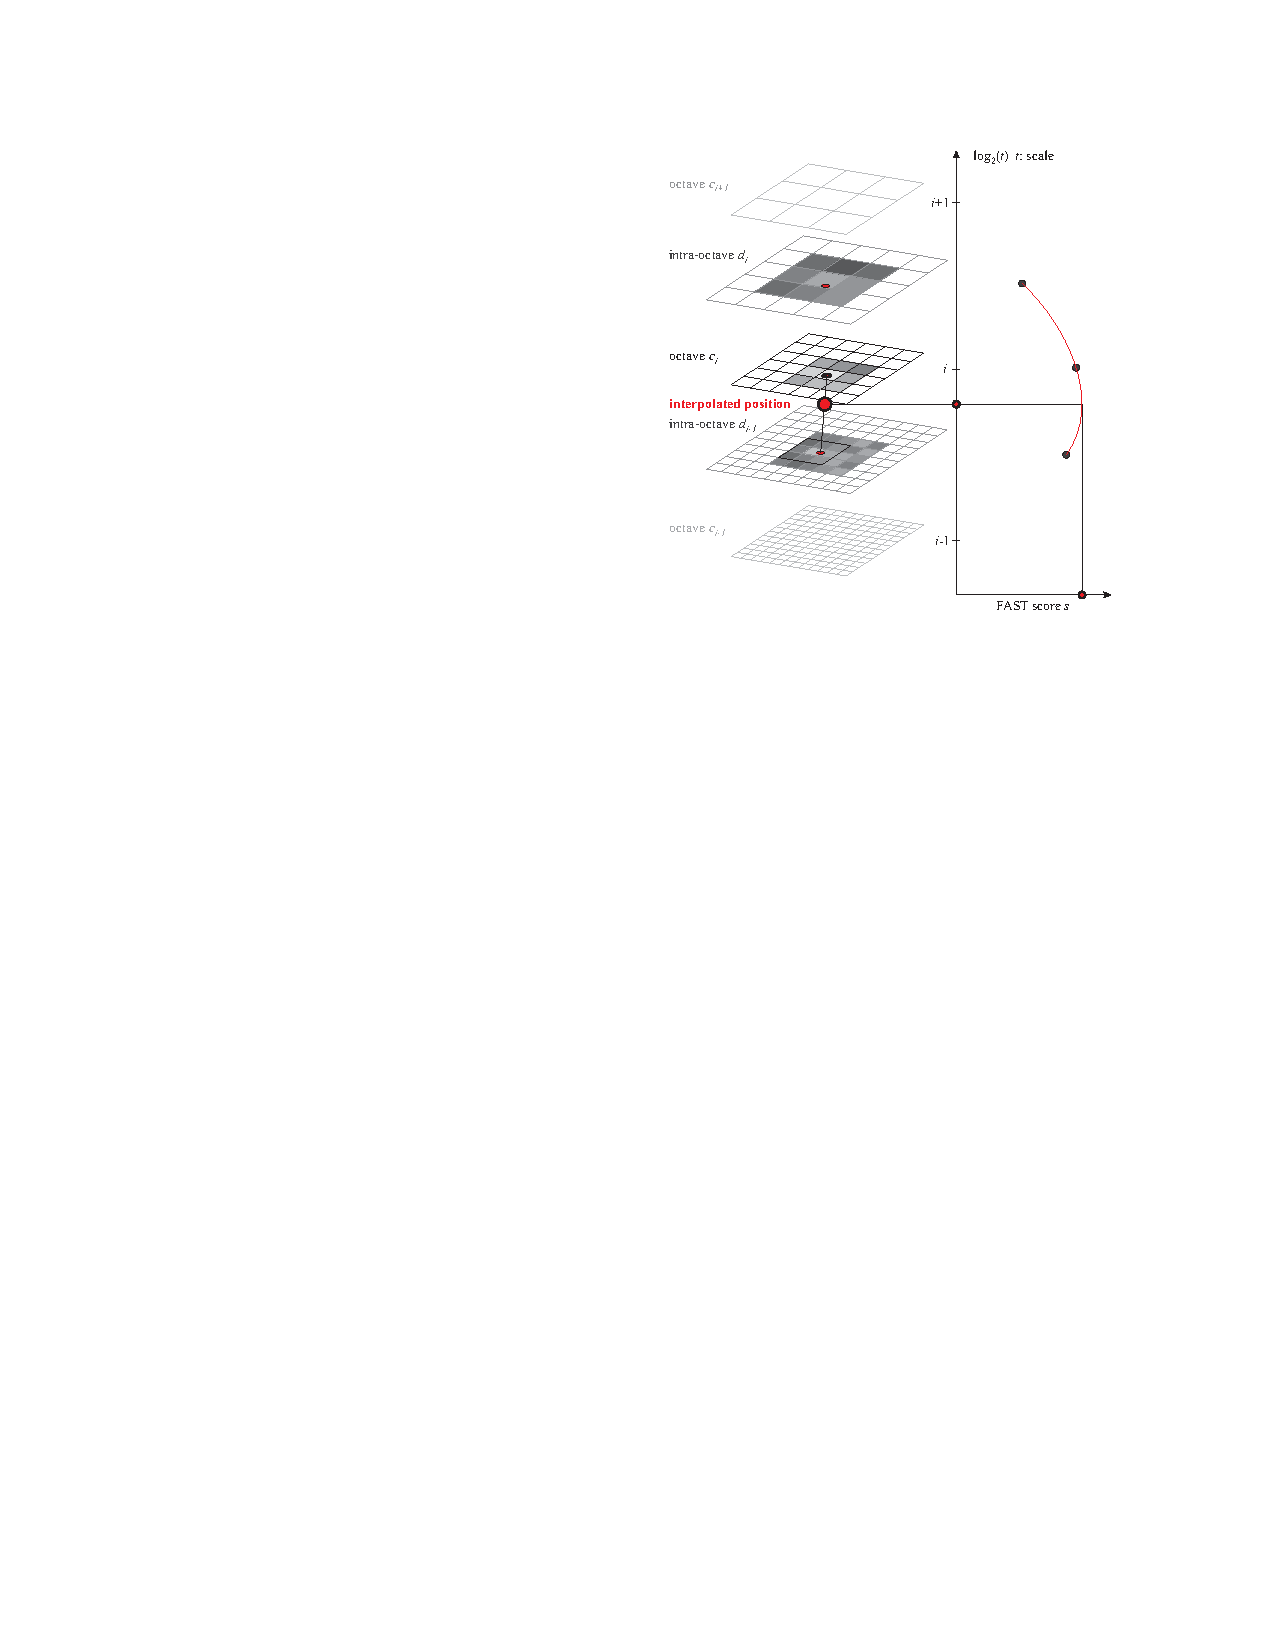
\includegraphics[width=0.8\textwidth]{../Drawings/methods/BRISKScaleSpace.pdf}
    \caption{Sub-pixel refinement and scale refinement is performed by interpolating a 1D parabola along three separate scales.}
    \label{fig:1dparabola}
\end{figure}

This procedure is performed on all detected maxima and this produces a set of interest points with sub-pixel refined image locations as well as true scale values. The descriptors for these interest points are subsequently determined.

\subsubsection{Descriptor}
\label{sec:briskDescribe}
One of the important aspects of the BRISK descriptor is that it uses a pre-determined pattern to sample the neighborhood surrounding each detected interest point $k$. Equally spaced samples, $p_i$ are chosen which are placed on concentric circles centered on the interest point. This is shown in \figref{fig:samplingPattern} \cite{Leutenegger2011}. Aliasing can occur and in order to prevent this problem, Gaussian smoothing is applied to each sampled point on the concentric circles with standard deviation $\sigma_i$ proportional to the difference between the sampled points on the circle. \\

\begin{figure}[h!] 
  \centering
    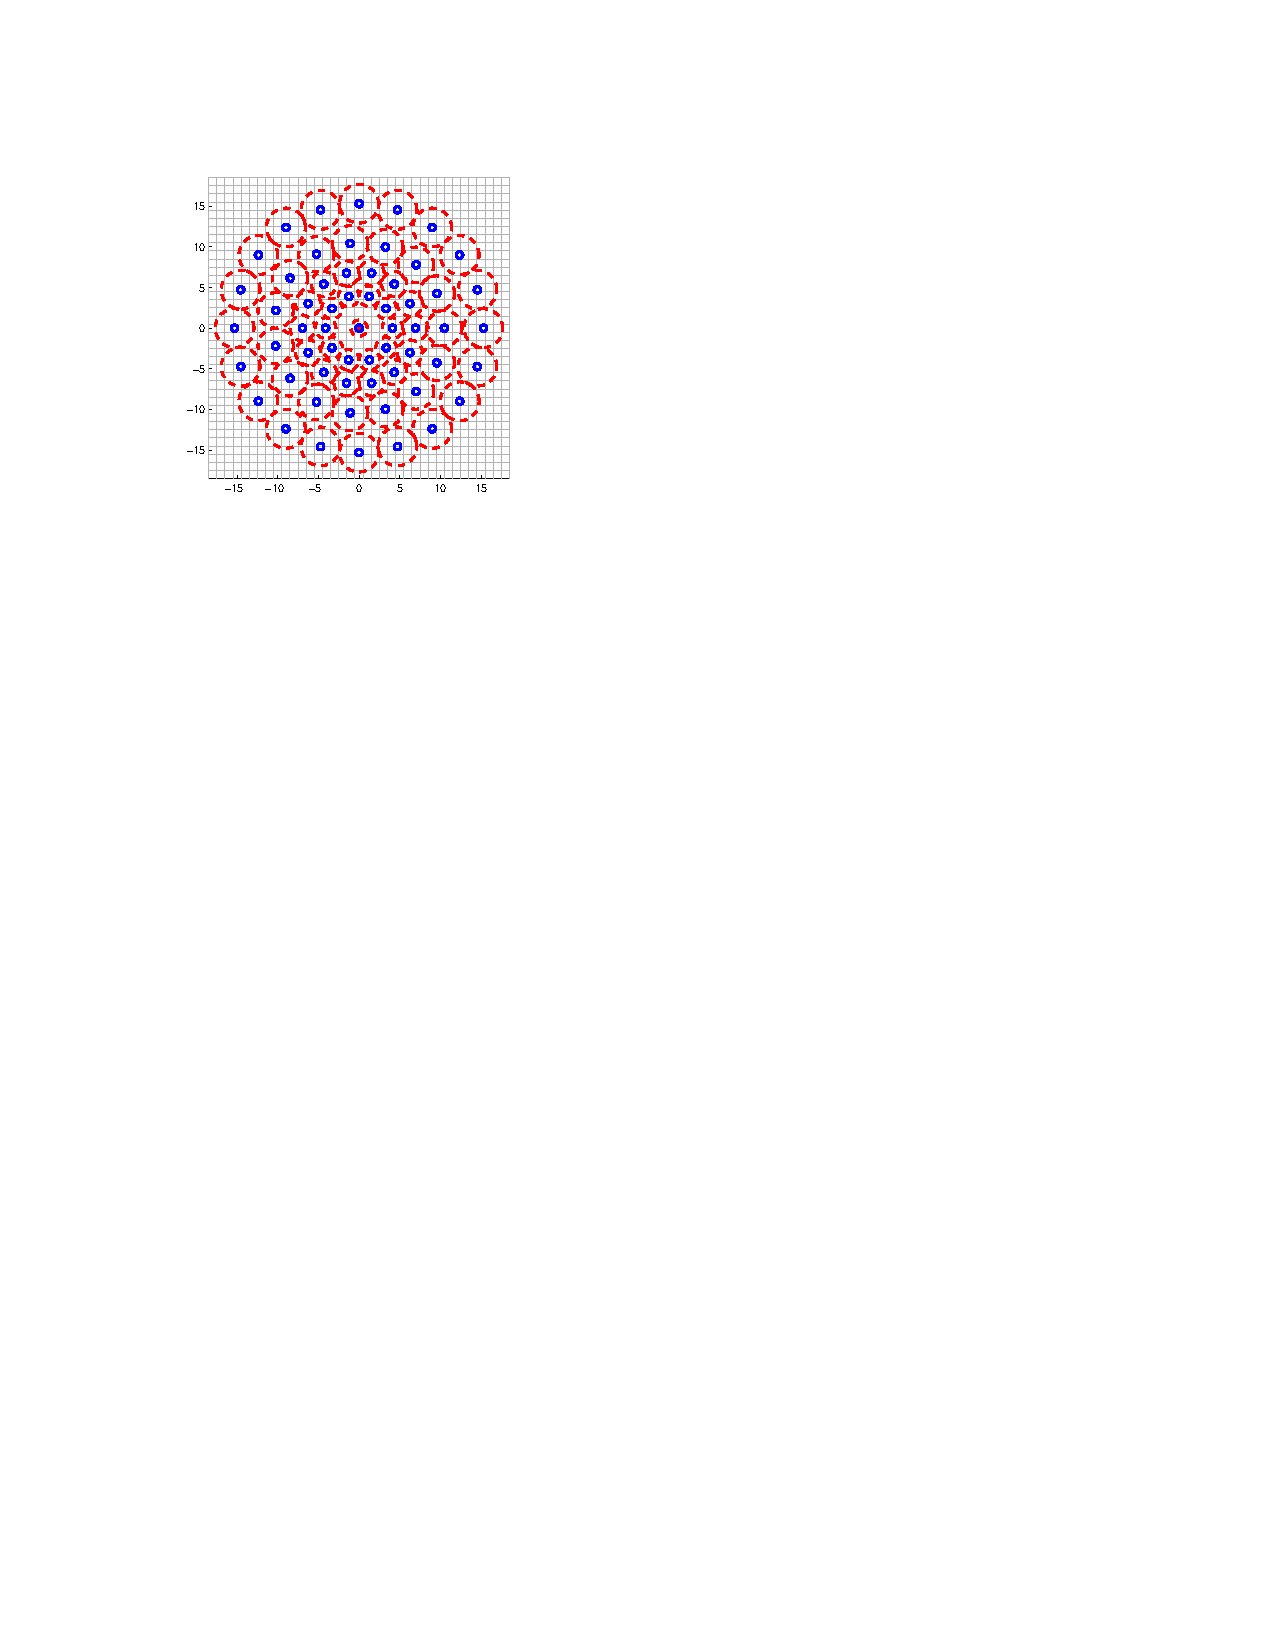
\includegraphics[width=0.8\textwidth]{../Drawings/methods/BRISK_Sampling_Pattern.pdf}
    \caption{The sampling pattern for an interest point. Each blue circle represents a sample and the red circle size is proportional to the amount of smoothing performed on each respective sample.}
    \label{fig:samplingPattern}
\end{figure}

The next step is to position and scale the pattern according to the interest points that has been detected. The first step in the procedure is to calculate the gradient between each of the points $(p_i, p_j)$ in the pattern. This gradient is calculated as shown in \eqnref{eqn:gradient}.\\

\begin{equation}
m(p_i, p_j) = (p_j - p_i) \frac{I(p_j, \sigma_j) - I(p_i, \sigma_i)}{||p_j - p_i||^2}
\label{eqn:gradient}
\end{equation}

Following this, the euclidean distance between all possible pairings of the sample points are computed to generate long and short pairs, $L$ and $S$ respectively. The pairings are defined as shown in \eqnref{eqn:pairings}. The thresholds $ \delta_{max},  \delta_{min}$ are chosen as $9.75h$ and $13.67h$ where $h$ is the scale of the interest point $k$. \\   


\begin{eqnarray}
S &=& ((p_i, p_j) \mid ||p_j - p_i|| < \delta_{max})\\
L &=& ((p_i, p_j) \mid ||p_j - p_i|| > \delta_{min})
\label{eqn:pairings}
\end{eqnarray} 

The overall pattern direction for the interest point is determined by computing the overall gradient of all the long pairings $L$ as shown in \eqnref{eqn:longGradients}. Long pairings are used instead of short pairings as it was found that short pairing gradients tend to cancel each other out \cite{Leutenegger2011}. \\

\begin{equation}
\textbf{M} = (m_x, m_y) = \frac{1}{L} \sum_{((p_i, p_j) \epsilon L)} m(p_i,p_j)
\label{eqn:longGradients}
\end{equation}

This gradient is then used to find the angle with which to rotate the sampling pattern around the interest point in order to achive rotation invariance. The angle is computed as shown in \eqnref{eqn:angle}. \\

\begin{equation}
\alpha = atan(\frac{m_y}{m_x})
\label{eqn:angle}
\end{equation}

Once the pattern has been rotated, the descriptor vector is computed. This vector is $512$ bits long and is formed using intensity comparisons between the rotated short distance pairings $S$. Therefore, for each short-distance pairing, a brightness comparison test as shown in \eqnref{eqn:brightness} is performed to yield the descriptor entry $d_k$, $k = 1,2,3...512$.\\

\begin{equation}
d_k = \left\{ \begin{array}{rl}
1 &\mbox{$I(p_j^{\alpha}, \sigma_j) > I(p_i^{\alpha}, \sigma_i)$,} \\
0 &\mbox{Otherwise}
\end{array} \right.
\label{eqn:brightness}
\end{equation}

This produces the rotation and scale invariant descriptor vector.\\ 

\section{Robocup Feature Extraction Techniques}
\label{sec:realtimeFeatureExtraction}

\subsection{BRISK0 - UBRISK}
\label{sec:brisk0}
In order to make the BRISK algorithm suitable for the Robocup domain, some slight modifications had to be made to the original algorithm. These changes include combining a detector defined as BRISK0, which is a slight variation of the original BRISK implementation, with a variety of Descriptors which will be described below. These feature extraction algorithms are applied to a gray-scale image and matching is performed using Hamming distance as described in \secref{sec:matching}.\\

\subsubsection{Image Processing}
\label{sec:imageProcessingBrisk}
In the Robocup scenario, when observing features, the robot's head will be tilted upwards at the maximum possible angle in order to observe features that are on or near the ceiling. This is because in a real Robocup environment, dynamic objects such as humans will generate volatile features. These feature are not necessarily repeatable and will potentially hinder the robot's localisation ability.\\

In order to improve the chances of generating non-volatile features, only the section of the image above the robot's horizon line is evaluated. This will effectively remove the dynamic background clutter that is found below the horizon line. In addition to the advantage of generating potentially non-volatile features, evaluating only a sub-section of the image results in a significant increase in computational performance. \\ 

\subsubsection{Detector}
\label{sec:BRISK0Detect}
The BRISK detector typically detects features by progressively half-sampling an image and in doing so creates a scale-space pyramid as defined in \secref{sec:brisk}. Creating this pyramid is computationally expensive but generates robust scale-invariant interest points.\\

The scale-space pyramid is not needed for this application and thus interest points are only detected along a single scale. This is achieved by setting the number of octaves to $0$ on the BRISK detector, effectively creating BRISK0. This causes the scale-space pyramid to be `flattened' to a single layer which is utilised to detect interest points. The effect of this is that FAST scores are only computed for a single layer and thus a non-maximal suppression is only performed on this layer in scale space. This results in a significant increase in computational performance. \\

%In addition to this, more features will be detected as the constraint required for detecting an interest point has been relaxed. This is also useful since regions around the ceiling do not usually have a large amount of variation and thus the amount of interest points detected will be relatively limited.\\

A 2D sub-pixel refinement is still applied to the interest points on the single layer resulting in an increased accuracy in interest point image coordinates.\\

Since only a single octave is utilised and interest points are therefore only detected on a single scale, the 1D parabola that is fitted along the scale-space axis \cite{Leutenegger2011} is also discarded. The disadvantage of this approach is that the local maxima FAST scores are not as accurate as in the original implementation but the increase in accuracy is not crucial in this application as good performance is still obtained as shown in \secref{sec:overallPerformance}. Furthermore, the increase in computational performance is crucial in developing a method that is practically implementable on the robot. This generates a bank of interest points and the descriptors are then computed.\\

\subsubsection{Descriptor}
\label{sec:BRISK0Describe}
In order to determine the best feature extraction algorithm to be utilised on the robot, a variety of BRISK and SURF descriptors have been combined with the BRISK0 detector. The descriptors include BRISK0, U-BRISK and 2D SURF descriptors respectively.\\

The BRISK0 descriptor complements the BRISK0 detector as assigns the same scale to all of the interest points. This is because interest points are detected on only a single scale as mentioned previously. The rest of the BRISK algorithm is computed according to the original BRISK implementation resulting in a rotation invariant descriptor of length $512$ bits\cite{Leutenegger2011}.\\

The SURF 2D descriptor is also combined with the BRISK0 detector. This creates a descriptor vector of length $64$ as implemented in 2D SURF \cite{Bay}. No modifications have been made to the SURF descriptor resulting in the same output as 2D SURF.\\ 

The U-BRISK descriptor contains a slight modification to the original BRISK descriptor. The rotation of the sampling pattern, which was described in \secref{sec:briskDescribe}, has been discarded. This removes the rotation invariant property of the BRISK feature extraction algorithm, but provides a significant increase in computational performance. The brightness comparison tests used to create the descriptor vector are therefore performed on interest points with a sampling pattern that remains in a standard orientation. The combination of BRISK0 and U-BRISK produces the best overall performance for the Robocup scenario as detailed in \secref{sec:overallPerformance}. \\

\subsection{1DSURF}
\label{sec:1dsurf}
Another technique that can be utilised for the Robocup is the 1D SURF feature extraction algorithm that has been previously implemented \cite{Anderson} for use in the Robocup. This algorithm extracts features from a single row of pixels in an image $A$. These features are then matched with features extracted from a row of pixels generated from an image $B$ being compared to image $A$. This technique is many orders of magnitude faster than the traditional 2D SURF implementation and is potentially suitable for use in the Robocup \cite{Anderson}.\\

In order to utilise the feature extraction algorithm, it had to be implemented according to the design detailed in \cite{Anderson}. The OpenSURF implementation, which is freely available online \cite{opensurf} has been utilised in order to implement this algorithm.\\

The main task is transforming 2D SURF into its 1D SURF implementation. This requires changes to both the detector and Descriptor and will be explained in the sections to follow.\\

\subsubsection{Image Processing}
\label{sec:imageProcessing}
The first main step in implementing the 1D SURF algorithm is to extract a single row of gray-scale pixels from the image. This is achieved by sampling every fourth pixel intensity value along the robot's horizon line in order to speed up processing time \cite{Anderson}. 
In addition to this, each sampled pixel intensity value is summed with a vertical band of $30$ pixels as shown in \figref{fig:rows}. This is performed instead of taking the mean primarily since it is faster to compute. This procedure therefore ultimately generates a row of summed pixel intensities. It is from this row of intensities that features will be extracted and matched.\\

\subsubsection{Detector}
\label{sec:1dsurfDetect}
The 1D SURF detector has a number of differences from that of its 2D equivalent. The first major difference is the construction of the integral image. The integral image as stated in \secref{sec:integralImages}, allows for fast computation of rectangular areas in an image. Since the image is now 1D, the integral image is only computed along the single row of pixels.\\ 

The next step is calculating the blob response for each point $(x,1)$ along the single row of pixels. In the 2D case, this is typically achieved by performing a 2D convolution, convolving a second order Gaussian derivative with the image at the point $\textbf{x} = (x,y)$. The Gaussian is approximated as a box filter and, combined with the integral image, results in a very efficient computation. In the 1D case, the convolution can only be computed along the single dimensional row of pixels. Thus the box filters have been effectively reduced to 1D box filters and the $xy$ and $y$ directional box filters can be neglected. The determinant of the Hessian can thus be reduced to \eqnref{eqn:reducedHessian}.\\

\begin{equation}
det(Hessian) = D_{xx}D_{xx}
\label{eqn:reducedHessian}
\end{equation} 

The number of octaves chosen for 1D SURF is $4$ and the number of scales per octave is $3$. Once a blob response map has been generated, interest points can be subsequently computed for each octave and each scale within the respective octave. Typically, in order to identify local maxima, each pixel in 3D scale space is compared to its $3 \times 3 \times 3$ surrounding neighbors and a non-maximal suppression is performed \cite{Evans2009}. However, in the case of 1D SURF, this constraint is relaxed and the pixel is only compared to its neighbors in the single scale space dimensional as shown in \figref{fig:singleScale} \cite{Anderson}. The result is that more features will be detected. However, these features will not have as strong responses as the features detected in 2D SURF.\\

Once this has been achieved, the interest points are usually interpolated in both scale and image space to sub-pixel accuracy \cite{Evans2009}. However, sub-pixel accuracy is not necessary for the Robocup domain and has thus been discarded in the 1D implementation \cite{Anderson}. This procedure ultimately detects a set of interest points along a single row of pixels based on the blob response map. The next step involves computing the descriptors.\\  

\subsubsection{Descriptor}
\label{sec:1dsurfDescribe}
Typically, the 2D SURF descriptor is constructed in two stages. The first stage involves assigning an orientation to the descriptor and has been described in \secref{sec:2dsurfdescribe}. This step has been discarded since the feature points are assigned with reference to the horizon line and therefore do not require an orientation.\\

In 2D SURF, the second stage involves constructing a square region around the interest point and sub-dividing the region into $16$ equally-sized sub-regions as detailed in \secref{sec:2dsurfdescribe}. For each sub-region, HWRs in both the $x$ and $y$ directions are calculated for $25$ regularly spaced sample points. These responses are summed together to produce $4$ descriptor values for the sub-region corresponding to \eqnref{eqn:descriptorSub}. Therefore, in total a descriptor vector of length $64$ is created.\\

In the case of 1D SURF, it is only possible to utilise $4$ of the $16$ sub-regions along the $x$ direction as shown in \figref{fig:subregions4} due to the reduction in dimensionality of the image. In addition, HWRs can only be calculated along the $x$ direction which allows for the $y$ direction Haar Wavelets to be discarded. The current implementation of 1D SURF further reduces the number of sub-regions to $3$ while still achieving good performance \cite{Anderson}. This will ultimately produce a $6$ dimensional descriptor vector rather than the $64$ dimensional descriptor vector as shown in \eqnref{eqn:descriptor1d}. Each of the $3$ sub-regions will produce a descriptor pair of $[\sum dx_i, \sum |dx_i|]$ where $dx_i$ refers to the HWR from the $i^{th}$ sub-region in the $x$ direction. \\

\begin{equation}
descriptor = [ \sum dx_1, \sum |dx_1|,\sum dx_2, \sum |dx_2|,\sum dx_3, \sum |dx_3|] 
\label{eqn:descriptor1d}
\end{equation}

\section{Feature Matching}
\label{sec:matching}

\subsection{Calculating Distance between Feature Descriptors}
\label{sec:distance}

\subsubsection{Hamming Distance}
\label{sec:hamming}
The Hamming distance is a metric that is used to indicate the difference between two strings \cite{Banzal2007}. Assume that there are two strings $A$ and $B$ of equal length. In this example, these strings can only take values of $0$ or $1$. The hamming distance is then calculated by determining whether or not the values of corresponding elements in each of the strings are different. If the values are different, then the hamming distance is incremented by a value of $1$.\\

This metric is used to determine the distance between feature descriptors in the BRISK algorithm \cite{Leutenegger2011}. Since the feature descriptors, as mentioned in \secref{sec:briskDescribe}, are vectors of $512$ bits in length, the Hamming distance of two feature descriptors is calculated by determining how different the first feature descriptor is from the other. It is desired that the feature descriptors are as similar as possible for the descriptors to be a match; that is, they have a very low hamming distance. \\

This is a very efficient algorithm and has been effectively performed in BRIEF \cite{Calonder}. It consists of $512$ XOR operations between corresponding bits followed by a bit count. This is a very efficient computation to perform on modern day architectures \cite{Leutenegger2011}. \\ 

\subsubsection{Euclidean Distance}
\label{sec:euclidean}
In SURF-based approaches,  the Euclidean distance is used as a metric to determine whether or not there is a match between two feature descriptors \cite{Lowe2004}. Given two feature descriptors of length $64$, the Euclidean distance is calculated and results in a value indicating the difference between the two feature descriptors. As in BRISK, it is desired that the Euclidean distance is as small as possible between the descriptors for them to be a match. A match occurs if the nearest neighboring feature descriptor corresponding to an interest point in image $A$ is within a specified euclidean distance from the descriptor of the corresponding interest point in image $B$.\\

In addition to this, in order to speed up matching, the sign of the Laplacian, which is the trace of the Hessian matrix is used to determine whether or not each blob response in the respective images are of a similar contrast \cite{Bay2008}. The sign of the Laplacian determines whether the interest point in question is a dark blob on a light background or a light blob on a dark background. This enables interest points of different contrasts to be rejected as matches without having to compute the euclidean distance between the points.\\

\subsection{Feature Matching Techniques}
\label{sec:matchingTechniques}
Two main feature matching techniques have been utilised in this implementation. Both BRISK and SURF-based approaches make use of 2-Nearest Neighbors and radius matching. A third technique has been implemented called the Edit-Distance constraint but has not been utilised as the first two techniques yield acceptable performance as will be discussed in \secref{sec:experimentsResults}. These feature matching techniques assume that interest points with corresponding feature descriptors in image $A$ (query image) are being compared to interest points with their corresponding descriptors in image $B$ (stored image). \\

\subsubsection{2-Nearest Neighbours Matching}
\label{sec:knn}
The 2-Nearest Neighbors (2-NN) feature matching technique involves finding the two feature descriptors in image $B$ that yield the closest matches respectively, in decreasing order, with the feature descriptor that is currently being queried in image $A$. This technique ensures that two matches will be found for every interest point in the query image $A$. Therefore the number of matches is always twice the total number of interest points in the query image. This does not cause a problem since these matches then have to go through a number of validation procedures detailed in \secref{sec:validation} in order to verify that the matches are indeed valid matches. Invalid matches are discarded. \\

The algorithm is implemented as follows. Initially all of the feature descriptors in the query and stored image pair are sent into the 2-NN matching algorithm. The hamming/euclidean distance (depending on the method) between each query descriptor and all of the stored descriptors is then calculated. The top two stored descriptors yielding the lowest hamming/euclidean distance are assigned as matches to the query descriptor. These matches are stored in descending order where the first match has the lower of the two distances.\\ 

\subsubsection{Radius Matching}
\label{sec:radius}
Radius matching is different from 2-NN in that a match between two feature descriptors only occurs if the calculated hamming or euclidean distance (depending on the feature extraction algorithm being used) is below a pre-defined threshold. This threshold is denoted the `Hamming Distance' for BRISK-based algorithms and the `Euclidean Distance' for SURF-based algorithms. \\

This method does not guarantee that every interest point in the query image will have a corresponding match in the stored image. Therefore it is possible that an interest point in the query image may have no matches with the interest points in the stored image.\\

The radius match algorithm is therefore given all of the interest point feature descriptors in both the query and stored images respectively. The descriptors are then matched based upon the pre-defined threshold. If a descriptor has more than one match, then these matches are sorted and stored in descending order where the first match has the smallest Hamming/Euclidean distance with the respective feature descriptor that is being queried.\\ 

\subsection{Edit-Distance Constraint}
\label{sec:editDistance}
An important observation that has been made is that if the same features are observed in images from two different views, they will still be viewed in the same order in both images. This assumes that either image has not been drastically rotated such that the features appear in a different order. This is a valid assumption in the case of the Robocup as the Nao is not subject to drastic rotations when coming onto the field after serving a penalty ban.\\

\textbf{TO DO}
%The Edit-Distance algorithm is a useful matching algorithm
%
% that imposes two important constraints \cite{Way1996}. The first constraint is that of \textit{Uniqueness}. This means that a feature in the query image can match only a single feature in the stored image. The second constraint is that of \textit{Monotonic Ordering}. This means that if a feature $f_{i_1}$ is matched to a feature $f_{i_2}$, then the next feature $f_{i_1 + 1}$ can only be matched to a feature $f_{i_2 + j}$ where $j \gt 0$. 


\subsection{Validating Matched Features}
\label{sec:validation}

\subsubsection{2-Nearest Neighbors Criterion}
\label{sec:knnMatching}
A constraint has been previously utilised to reject invalid matches. This constraint is called the 2-NN Ratio and is computed between the closest and second closest match for a particular interest point \cite{Lowe2004}. This is performed for every detected interest point in the image being evaluated. It has been assumed that each interest point has only a single, unique corresponding match between a pair of images. Based on this assumption, the first 2-NN match should be the true matching interest point in the corresponding image, whereas the second 2-NN match should belong to a different object in the image and hence is an invalid match.\\

Therefore, for a valid match between interest points, the closest match should be significantly closer than the second closest match (which is the closest incorrect match) from the interest points that is being evaluated \cite{Lowe2004}. This means that a valid match should generally have a lower 2-NN ratio than an invalid match. An invalid match will probably have a number of matches within a similar distance of one another due to the high dimensionality of the feature space \cite{Lowe2004}. The feature space, as mentioned previously is of dimensionality $64$ for 2D SURF and $512$ for BRISK-based techniques.\\

Based on the results in \secref{sec:knnMatchingConstraint}, all matches with a threshold above $0.7$ are rejected as invalid matches whereas all matches with a threshold below this value are accepted as valid matches.\\



\subsubsection{Angle and Distance Constraints}
\label{sec:angleDistanceConstraints}
Two new matching constraints have been developed in order to determine whether or not a match between two interest points in corresponding images are valid, namely, the angle and distance constraints respectively. A pair of interest points have to fulfil both of these constraints in order to be considered a valid match. In order to verify that the match fulfils these constraints, the pair of images that are being evaluated are placed side by side one another as shown in \figref{fig:imagesSide}. After placing the images next to one another, a line is connected between each set of matched interest points. In the figure below, there is only a single match. The angle from the interest point in the left image is calculated relative to the interest point in the right image. If the angle is too large, then the match is invalid and is discarded.\\

\begin{figure}[h!] 
  \centering
    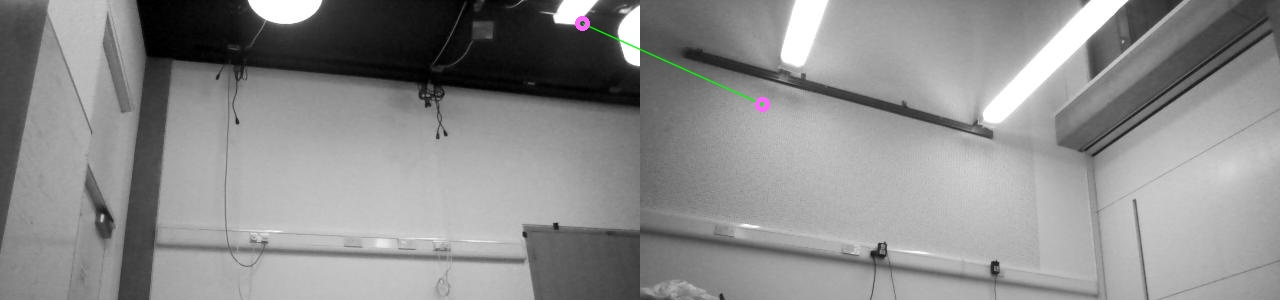
\includegraphics[width=0.8\textwidth]{../Drawings/constraints/t_20_hd_55_OG_Left_MG_Right_2_12.jpg}
    \caption{An incorrect match detected due to an angle larger than $10^\circ$}
    \label{fig:imagesSide}
\end{figure}

\subsubsection{RANSAC Constraint}
\label{sec:ransacConstraint}




\section{Localisation Algorithm}
\label{sec:localisation}
The Nao robot is able to perform localisation as it is initially given a map of the Robocup soccer field. It typically uses features such as the goalposts, line segments and corners in order to localise itself on the field \cite{Bhuman}. There are a number of different localisation algorithms that have been previously implemented on the Nao to achieve localisation. The localisation algorithm utilised for this project is the \textit{Augmented} Monte Carlo Particle Filter \cite{Laue}.

\subsection{Augmented Monte Carlo Particle Filter}
\label{sec:amcpf}
The Augmented Monte Carlo Particle Filter (AMCPF) is simply an extension of the Monte Carlo Particle Filter (MCPF). The MCPF represents the belief or probability of the robot being in a certain position $x_t$ by $bel_{x_t}$ \cite{Thrun2002}. 


This project utilises a Monte Carlo Localisation (MCL) algorithm that has been implemented on the Nao \cite{Bhuman}. A specialised version of MCL has been utilised, called \textit{Augmented} Monte Carlo Localisation \cite{Laue}. This variation of MCL has the advantage of enabling the robot to overcome the \textit{kidnapping} problem, which occurs when the robot faces a \textit{Standard Removal Penalty}. This is achieved using random particle injection which occurs based on the ratio of the short and long-term measurement likelihoods as mentioned previously.\\

\subsection{Localisation using Natural Visual Features}
\label{sec:localisationNaturalVisualFeatures}
The first step in localising the robot occurs prior to the start of the game. The robot will initially capture a set of images behind each of the goal posts. The interest points will be detected using the relevant feature extraction algorithm and descriptors for these interest points will be computed and stored by the robot for the remainder of the game. It is assumed that these features are persistent throughout the game. However, this is the initial implementation and the features can be updated during the course of the game as a future improvement.\\

When a penalty occurs and a robot is removed from the field, it has to relocalise itself on re-entering the field. As mentioned previously, the robot is placed on the half-way line, the nearest spot from the half-way line or on its respective side of the field facing the opposition once the penalty period has ended. At this point, the robot receives a list of visual features that are present on the field. These include the goal posts, line segments, line crossings (intersections between line segments) and the center circle \cite{Bhuman}. These are illustrated in \figref{fig:features}.\\

Using these visual features, the robot knows that it is in one of two locations after processing these features in the AMCL algorithm. These scenarios are illustrated in \figref{fig:location}. If the robot enters the field and sees a goal post to its right, then its possible positions are represented by the red crosses. If the goal posts are to its left, then its positions are represented by the black crosses. At this point the robot needs to disambiguate between these choices of position.\\

\begin{figure}[ht!]
\begin{minipage}[b]{0.5\linewidth}
  \centering
    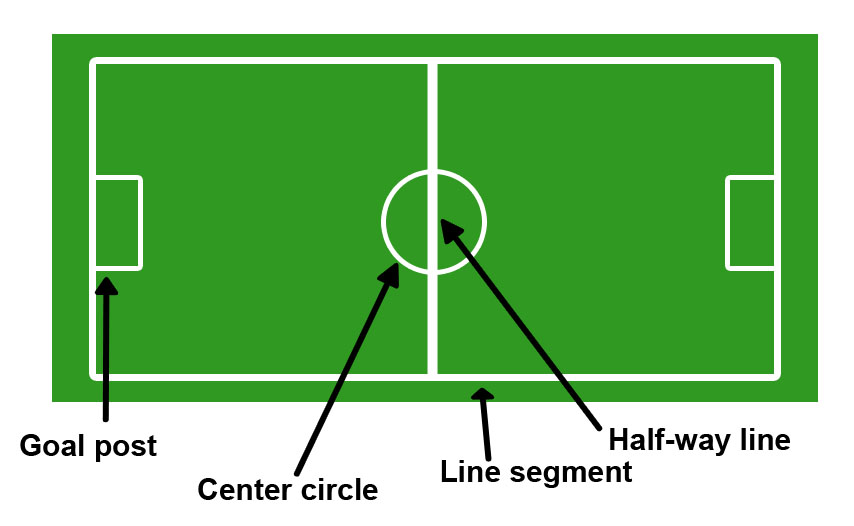
\includegraphics[width=0.6\textwidth]{../Drawings/localisation/goalSetup.jpg}
    \caption{The visual features available on the football field} 
    \label{fig:features}
\end{minipage}
\begin{minipage}[b]{0.5\linewidth}
  \centering
    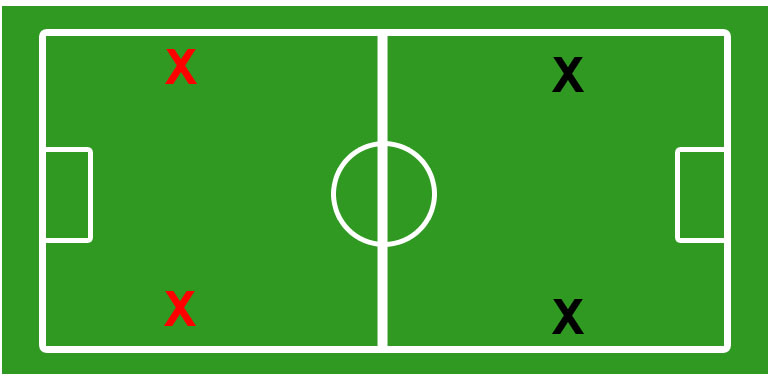
\includegraphics[width=0.6\textwidth]{../Drawings/localisation/possibleLocations.jpg}
    \caption{The possible locations where a robot might be on re-entering the field} 
    \label{fig:location}
\end{minipage}
\end{figure}

%Disambiguation step
%Discuss when it comes onto the field.
Once the robot has determined that it is in one of two locations on the field, it will then disambiguate its location using the persistent natural visual features that it identified at the start of the game detailed in \secref{sec:initialise}. At this point, the AMCL algorithm should have a set of particles with large weights in one of two potential locations. An example of this is shown in \figref{fig:before}. These images are screenshots captured in real-time using the SimRobot Simulator that has been designed by the Bhuman Robocup team \cite{Bhuman}.\\

\begin{figure}[h!] 
  \centering
    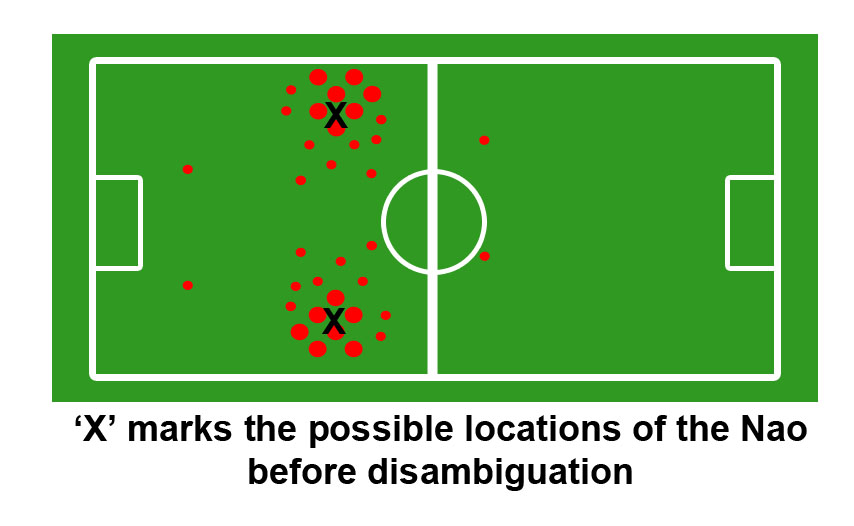
\includegraphics[width=0.8\textwidth]{../Drawings/localisation/beforeDisambiguate.jpg}
    \caption{Two possible positions are surrounded by particles with large weights.}
    \label{fig:before}
\end{figure}

The robot then compares its database of natural visual features computed prior to the start of the game, with the natural visual features that it identifies on re-entering the pitch. This situation is depicted in \figref{fig:featureMatching}. Here the robot identified features \textit{F1,F2,F3} above its goal and features \textit{F4,F5,F6} above the opponents goal prior to the start of the game. On re-entering the pitch, the robot compares the detected features from its current image of a goal with the features in its stored database of features. If it is able to match the new features that it sees with the stored features in its database, depicted by the red circles in the figure, then it will be able to determine its location relative to the field as well as its team's and opponent's goal posts respectively.\\

\begin{figure}[h!] 
  \centering
    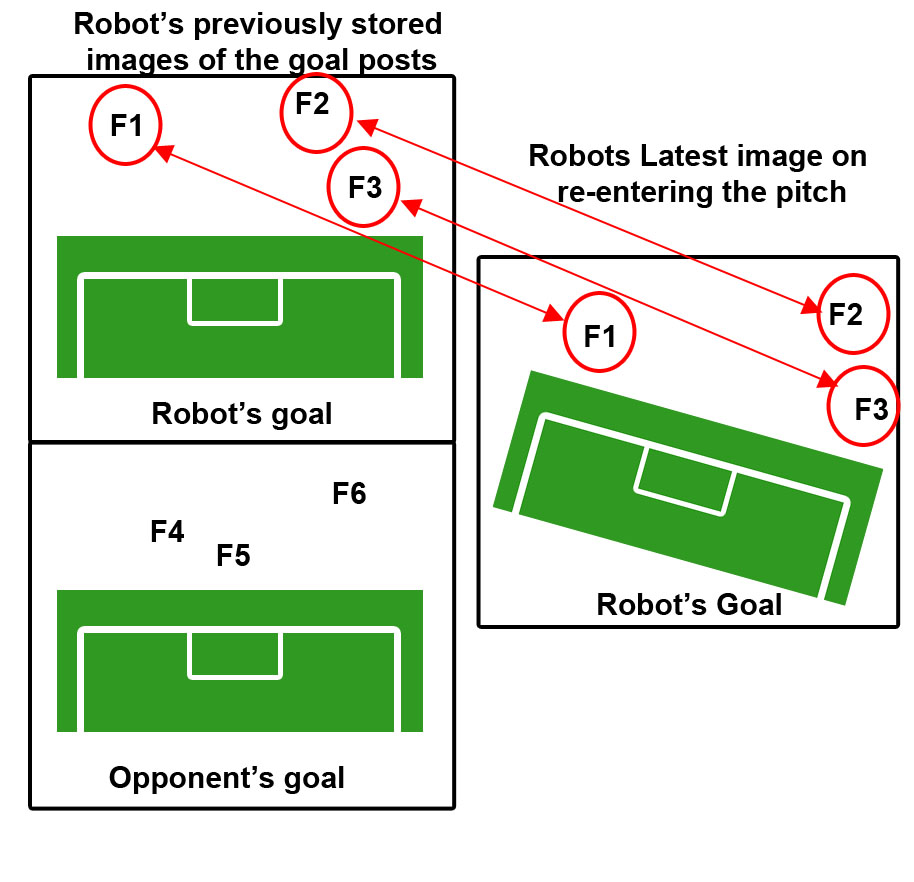
\includegraphics[width=0.8\textwidth]{../Drawings/localisation/featureMatching.jpg}
    \caption{Matching features to disambiguate position}
    \label{fig:featureMatching}
\end{figure}

The formal algorithmic procedure for disambiguation will be performed as follows. On re-entering the pitch, the robot will look to its left (arbitrarily chosen) and will identify features above the goal post using \textbf{\cite{Anderson}'s 1D SURF} implementation. The robot will then perform feature matching using nearest neighbors with ordering and scaling constraints as defined in \cite{Anderson}. Once the robot can associate a set of features with a particular goal post, it will be able to disambiguate its position on the field. The robot will disambiguate its position on the field by re-weighting the particles in the AMCL algorithm such that they represent the robots new posterior belief. Using \figref{fig:before} as the reference example, if the robot realises from the the natural landmarks that it is in the top right side of the pitch, the corresponding particles will be assigned larger weights resulting in the robot obtaining an estimate of its position. The resulting estimate is depicted in \figref{fig:after}. This reweighting of the particles is a proposed addition to the \textit{Augmented} AMCL algorithm and is depicted in red in \figref{fig:mclProposed}.\\

\begin{figure}[h!] 
  \centering
    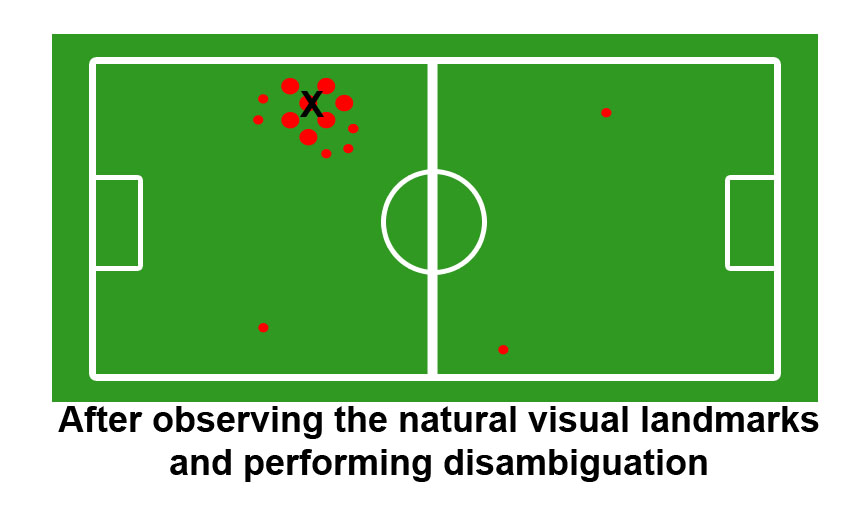
\includegraphics[width=0.8\textwidth]{../Drawings/localisation/afterDisambiguate.jpg}
    \caption{The robot's estimated position after disambiguation}
    \label{fig:after}
\end{figure}

\begin{figure}[h!] 
  \centering
    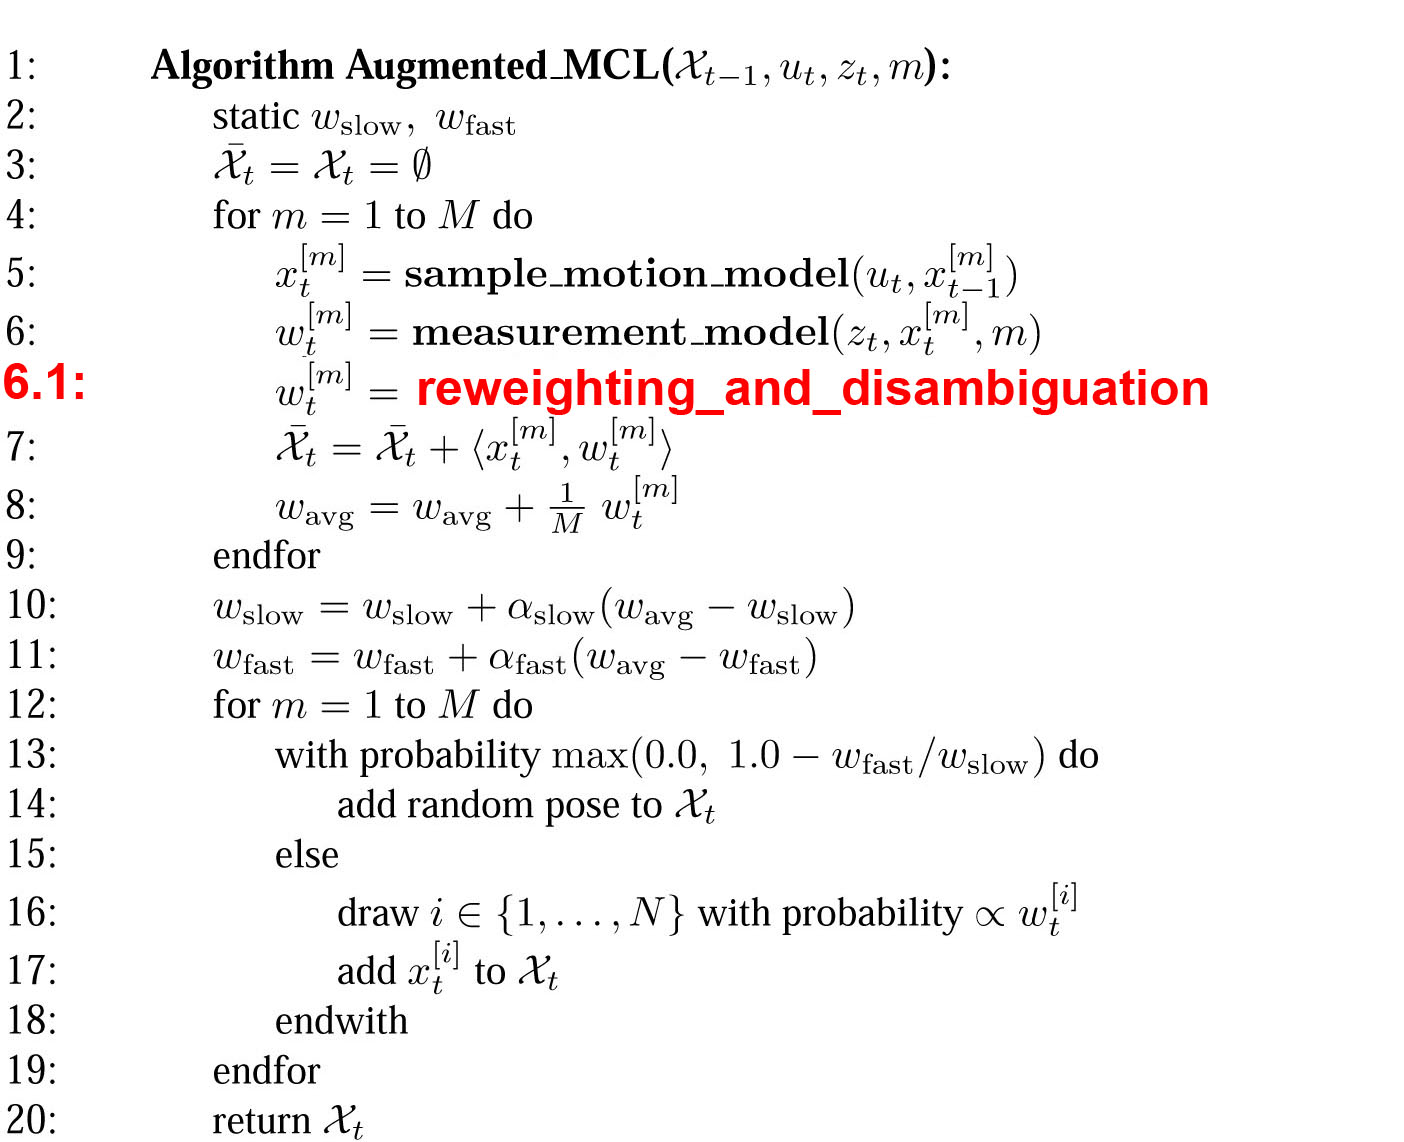
\includegraphics[width=0.8\textwidth]{../Drawings/localisation/MCLAugmented.jpg}
    \caption{The proposed implementation of the method in the Monte Carlo Algorithm \cite{Thrun2002}}
    \label{fig:mclProposed}
\end{figure}


%Discuss how the robot performs the localisation procedure.
%Briefly mention the fact that the robot relocalises itself using a re-weighting routine

\subsection{Re-weighting Particles and Importance Sampling}
\label{sec:reweighting}
%This is where the orientation algorithm is placed
An algorithm has been developed in order to effectively re-weight the particles.

\subsection{Bhuman Code Structure}
\label{sec:codeStructure}
%Discuss the basics of the bhuman code structure
%Include a basic diagram of modules, representations etc

\subsection{Natural Landmark Code Structure}
\label{sec:naturalLandmarkCode}
%Discuss how the Natural landmark detection has been placed into the bhuman code structure
%include a diagram from the simRobot interface


\section{Experiments and Results}
\label{sec:experimentsResults}
The experiments were conducted on a variety of feature extraction and matching algorithms. The feature extraction algorithms tested and compared in these experiments are BRISK0, BRISK, BRISK0-UBRISK, BRISK0-2D SURF and 1D SURF respectively. There are two types of matching techniques utilised for these experiments. They are 2-Nearest Neighbors and Radius Matching respectively. 2-Nearest Neighbors has been implemented on all of the feature extraction algorithms. All BRISK descriptors use hamming distance to perform radius matching whereas SURF descriptors rely on the euclidean distance to perform radius matching. All of the feature extractor algorithms are therefore compared based on their detection performance and descriptor generation as well as the matching technique that has been utilised for the particular experiment.\\

Parameters $p$ in this section correspond to the various thresholds required for detecting interest points and determining matches. The parameters used for each method are shown in \tabref{tab:parameters}. The Minimum Interest Point Detection Threshold (MIPDT) is the threshold above which a pixel is detected as an interest point. The Maximum Accepted Hamming Distance (MAHD) is the maximum number of bits that can differ when comparing two feature descriptors, below which the descriptors are to be considered a match. The Maximum Accepted Euclidean Distance (MAED) is the maximum euclidean distance below which two feature descriptors are considered to be a match.\\

\begin{table}
\caption{The parameters evaluated for each feature extraction algorithm}
\begin{tabular}{|c|c|c|}
\hline 
Method & Parameter 1 & Parameter 2\tabularnewline
\hline 
 & \multicolumn{2}{c}{2-Nearest Neighbors Matching}\tabularnewline
\hline 
BRISK0 & MIPDT & N/A\tabularnewline
\hline 
BRISK4 & MIPDT & N/A\tabularnewline
\hline 
BRISK0 SURF2D & MIPDT & N/A\tabularnewline
\hline 
BRISK0 - UBRISK & MIPDT & N/A\tabularnewline
\hline 
 & \multicolumn{2}{c}{Radius Matching}\tabularnewline
\hline 
BRISK0 & MIPDT & MAHD\tabularnewline
\hline 
BRISK4 & MIPDT & MAHD\tabularnewline
\hline 
BRISK0 SURF2D & MIPDT & MAED\tabularnewline
\hline 
BRISK0 - UBRISK & MIPDT & MAHD\tabularnewline
\hline 
\end{tabular}
\label{tab:parameters}
\end{table}

\subsection{Main Robocup Datasets and Setup}
\label{sec:datasets}
The setup for the feature extraction experiments is as follows. Four image datasets were generated. These images were taken from the Nao's camera at different angles and scales in order to ensure realistic images similar to those taken in a Robocup soccer game. All images were focused on the regions behind the goalposts. The first set of goalposts will be referred to as the Player's Goal (PG). The second set of goalposts will be referred to as the Opponents Goal (OG). \\


The first dataset is of the area to the left of the player's goal (\textit{PG Left}). The second dataset is to the right of the player's goal (\textit{PG Right}). The third dataset is to the left of the opponent's goal (\textit{OG Left}). The fourth dataset is to the right of the opponents goal (\textit{OG Right}). The abbreviations, shown in braces, will be used to refer to these datasets for the remainder of this report. Typical images from each of these datasets are shown in \figref{fig:dataset1} to \figref{fig:dataset4} respectively.\\

\begin{figure}[h!]
\begin{minipage}[b]{0.5\linewidth}
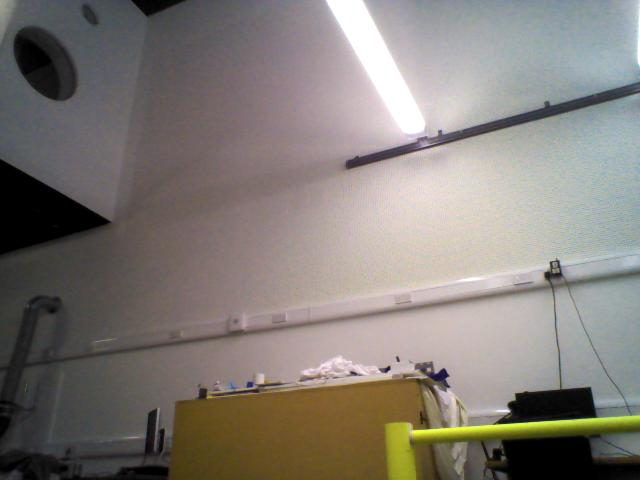
\includegraphics[scale=0.5]{../Drawings/datasetImages/mgLeft.jpg}
\caption{Dataset one showing an image from \textit{PG Left}}
\label{fig:dataset1}
\end{minipage}
\hspace{0.5cm}
\begin{minipage}[b]{0.5\linewidth}
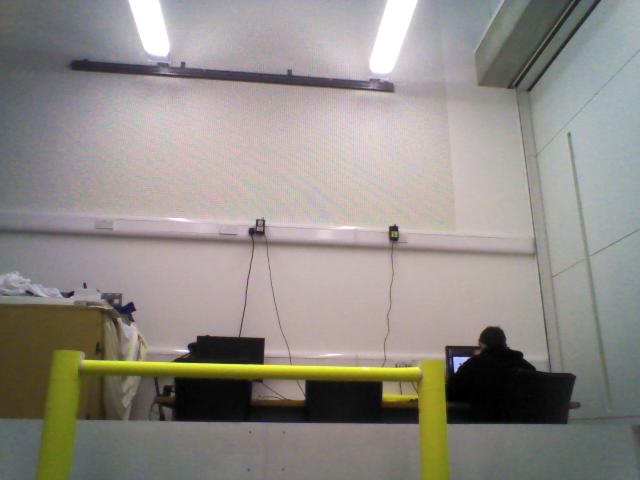
\includegraphics[scale=0.5]{../Drawings/datasetImages/mgRight.jpg}
\caption{Dataset two showing an image from \textit{PG Right}}
\label{fig:dataset2}
\end{minipage}
\hspace{0.5cm}
\begin{minipage}[b]{0.5\linewidth}
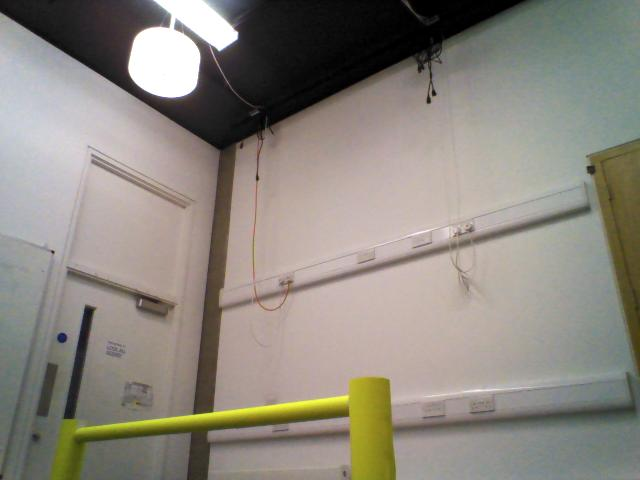
\includegraphics[scale=0.5]{../Drawings/datasetImages/ogLeft.jpg}
\caption{Dataset three showing an image from \textit{OG Left}}
\label{fig:dataset3}
\end{minipage}
\hspace{0.5cm}
\begin{minipage}[b]{0.5\linewidth}
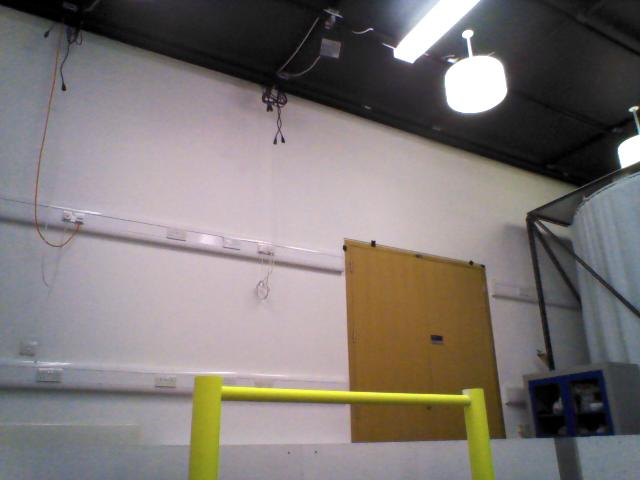
\includegraphics[scale=0.5]{../Drawings/datasetImages/ogRight.jpg}
\caption{Dataset four showing an image from \textit{OG Right}}
\label{fig:dataset4}
\end{minipage}
\end{figure}

Feature detection, extraction and matching routines were performed on pairs of images to determine whether the images match or not. Pairs of images taken from the same dataset are referred to as overlapping images. A pair of images are considered to overlap one another if at least $50\%$ of the first image visually overlaps the second image. Pairs of images, with no overlap, taken from different datasets are referred to as non-overlapping images. In order to ensure that images do not overlap, datasets from opposite sides of the soccer field were compared. Thus datasets \textit{PG Left} and \textit{PG Right} were compared with datasets \textit{OG Left} and \textit{OG Right} respectively as shown in \tabref{table:overlap}. \\

In total, $108$ overlapping images were used to generate $1421$ overlapping image pairs. A further $108$ non-overlapping images were used to generate $2808$ non-overlapping image pairs. This data has been utilised to generate the results in the sections to follow. \\ 

\begin{table}
\caption{Datasets and image combinations used for the comparison tests}
\begin{tabular}{|c|c|c|c|c|}
\hline 
Dataset A & Dataset B & Images in A & Images in B & Compared Image Pairs\tabularnewline
\hline 
\hline 
\multicolumn{5}{|c}{Overlapping Images}\tabularnewline
\hline 
1 & 1 & 26 & 26 & 325\tabularnewline
\hline 
2 & 2 & 28 & 28 & 378\tabularnewline
\hline 
3 & 3 & 31 & 31 & 465\tabularnewline
\hline 
4 & 4 & 23 & 23 & 253\tabularnewline
\hline 
\multicolumn{2}{|c|}{Total} & 108 & 108 & 1421\tabularnewline
\hline 
\multicolumn{5}{|c}{Non-Overlapping Images}\tabularnewline
\hline 
1 & 3 & 26 & 31 & 325\tabularnewline
\hline 
1 & 4 & 26 & 23 & 253\tabularnewline
\hline 
2 & 3 & 28 & 31 & 378\tabularnewline
\hline 
2 & 4 & 28 & 23 & 253\tabularnewline
\hline 
\multicolumn{2}{|c|}{Total} & 108 & 108 & 2808\tabularnewline
\hline 
\end{tabular}
\label{table:overlap}
\end{table}

\subsection{Feature Extraction Performance}
\label{sec:featureExtraction}
Before the feature extraction and matching algorithm can be implemented on the robot, the optimal feature extraction algorithm needs to be determined. In order to find the best algorithm, all of the feature extraction techniques need to be tested on the image datasets in order to find out which technique is the most consistent and accurate in disambiguating between different sides of the goal. \\

In order to find the optimal feature extraction and matching algorithm, the overlapping image pairs are initially used to determine the optimal parameters for each of the feature extraction algorithms. Once the optimal parameters have been found, both the non-overlapping image pairs and the overlapping image pairs are used to determine the matching performance of the respective feature extraction algorithm. The algorithm with the best performance will be implemented on the Nao robot.\\

\subsubsection{Finding the Optimal Detection Parameters}
\label{sec:optimalParameters}
%Describes how to find the optimal hamming distance, euclidean distance, and response thresholds for each method
The procedure used to determine the optimal parameters for each of the feature extraction algorithms will now be detailed. The parameters can be thresholds, hamming distances or euclidean distances as discussed in \secref{sec:matching}. Four datasets, presented in \secref{sec:datasets}, containing in total $108$ overlapping images were used to determine the optimum feature extraction parameters. All possible combinations of overlapping images were matched in datasets  one to four, without repetition, for various parameter values. A procedure has been developed in order to calculate the optimum parameters used to provide the best feature extraction and matching performance.\\
%The equation containing the optimal parameters
In order to find the optimal parameters, the Single Image Score (SIS) needs to be computed. This equation is shown in \eqnref{eqn:optimalParameters}. This matching score represents how good a match is between a pair of images, $i_1, i_2$ in a particular dataset $d$, for a particular Feature Extraction algorithm $FE$, using a certain set of parameters, $p$. For example, if the detector used is BRISK0, then the $SIS_{(i_1, i_2), d}^{BRISK0, \textbf{p}}$ presents the matching score for the pair of images $i_1, i_2$ for a specific detection threshold $p$ in a particular dataset $d$. \\

\begin{eqnarray}
SIS_{(i_1, i_2), d}^{FE, \textbf{p}} &=& \frac{k_1 f(t_{i_1,i_2}) + k_2 g_(\textit{NVM}_{i_1,i_2})}{k_1 + k_2} \\
k_1 + k_2 &=& 1  
\label{eqn:optimalParameters}
\end{eqnarray}

This matching score is composed of two normalised scoring functions, namely $f(t_{i_1, i_2})$ and $g(NVM_{i_1, i_2})$ shown in \eqnref{eqn:time} and \eqnref{eqn:nvm} respectively. $f(t_{i_1, i_2})$ represents the matching score for the pair of images $i_1, i_2$ for a particular dataset based on the overall time, $t$, taken to perform the image processing, detection, extraction and matching routines respectievly between these images. The unit of $t$ is milliseconds and the value of $t$ is normalised to a scale between $0$ and $1$. This is achieved by multiplying $t$ by $0.9$ and dividing this result by $t_{max}$ where $t_{max}$ is the largest time tabulated for the current dataset in milliseconds. A value of $0.1$ is then been added to this ratio in order to  prevent $log(0) = \infty$ which would largely bias the results as well as ensuring that the value $(\frac{0.9 t}{t_{max}} + 0.1)$ is normalised between $0$ and $1$. The function $f(t_{i_1, i_2})$ will ensure that, for large $t$, meaning that the algorithm takes a large amount of time to perform the routine, the matching score will be low, whereas for small $t$, the matching score will be high. \\

The second scoring function used to calculate the SIS is $g(NVM_{i_1, i_2})$. This scoring function rewards the pair of images $i_1, i_2$ if they contain a large amount of valid matches. This is intuitive as the more valid matches there are between two images, the more certain the match becomes. The variable $NVM$ represents the Number of Valid Matches (NVM) between two images. This function is normalised between $0$ and  $0.9$ by dividing this variable by the total amount of matches,$M_{total}$, generated from the pair of images $i_1, i_2$. The reason $M_{total}$ has been chosen as the normalisation factor is because it prevents a biased score. A biased score can occur in the following scenario. Assume that a pair of images $a_1, a_2$ generate a large amount of matches, but only a small proportion of these matches are valid. This is in contrast to another pair of images $b_1, b_2$ from the same dataset that generated a small set of matches, but a high proportion of valid matches. If $M_{total}$ was denoted as the maximum number of matches in the dataset, then images $b_1, b_2$ would have a smaller score than that of $a_1, a_2$ even though $b_1, b_2$ has a higher proportion of valid matches. Thus $M_{total}$ has been chosen to be the total number of matches between a pair of images $i_1, i_2$. This relative value largely prevent the biased scores. The value $\epsilon$ has been added to ensure that no infinite scores are computed. $\epsilon$ can take any value greater than $0$ and has been chosen to have a value of $0.1$ for these experiements.\\ 

The parameters $k_1$ and $k_2$ are weights that are used to bias the effects of the two scoring functions. Thus they can be used as controls to determine whether time or the number of valid matches should have a larger influence on the matching score. The weights sum to one and are used to normalise the SIS function.\\

\begin{equation}
f(t_{i_1, i_2}) = \mid log_{10}(\frac{0.9 t_{i_1, i_2}}{t_{max}^{FE}} + 0.1) \mid \quad f(t_{i_1, i_2})\epsilon [0, 1]
\label{eqn:time}
\end{equation}

\begin{equation}
g(NVM_{i_1, i_2}) = \frac{NVM_{i_1, i_2}}{M_{total, (i_1, i_2)} + \epsilon} \quad g(NVM_{i_1, i_2}) \epsilon [0, 0.9] %State that epsilon is between 0 and 1
\label{eqn:nvm}
\end{equation}

Once the SIS score has been calculated for each pair of images $i_1, i_2$ in a particular dataset for a particular feature extraction method and using particular values for the parameters, the scores are then summed together for each specific set of parameter values. The resulting score is called the Multi-Image Score (MIS) and is shown in \eqnref{eqn:mims}.\\

\begin{equation}
MIS_{p, d}^{FE} = \frac{k_3 \frac{\sum_{i_1, i_2=1 , i_1 \neq i_2}^{N} \textit{SIS}_{(i_1, i_2),d}^{FE,p}}{N} + k_4 h(\textit{NZM})}{k_3 + k_4}
\label{eqn:mims}
\end{equation}

As mentioned above, the MIS score is computed for a particular set of parameter values $p$ using a specific feature extraction algorithm $FE$ in  a particular dataset $d$. \\

The first term in the equation is the computation of the mean of all SIS scores for a particular set of parameter values. A function has been introduced to account for the Number of Zero Matches (\textit{NZM}) for a particular set of parameter values. A \textit{NZM} is defined as a pair of images containing no valid matches. The function $h(NZM)$, defined in \eqnref{eqn:nzm}, determines the number of \textit{NZMs} in a particular dataset $d$, for a particular set of parameter values $p$ using feature extraction algorithm $FE$. This equation has the same form as equation \eqnref{eqn:time} and therefore behaves in the same way. However, in this case the denominator $\textit{NZM}_{max}^{FE}$ represents the maximum number of NZMs found for a particular threshold in particular dataset using a particular feature extraction algorithm. This function therefore penalises parameter settings that result in a large number of \textit{NZM}s since \textit{NZM}s should not be present in a dataset of overlapping images. \\

\begin{equation}
h(\textit{NZM})_{p, d}^{FE} = \mid log_{10}(\frac{0.9\textit{NZM}_{p}^{FE}}{\textit{NZM}_{max}^{FE}} + 0.1) \mid \quad h(\textit{NZM}_{p}^{FE})\epsilon [0, 1]
\label{eqn:nzm}
\end{equation}

The MIS score contains another set of weighting parameters, $k_3$ and $k_4$, that can again be used to control the influence of each term in the function. These weights add up to one.\\

\eqnref{eqn:mims} therefore provides an overall score of how well images are matched for a specific setting of parameter values $p$ in dataset $d$ using feature extraction algorithm $FE$. \\

There is more than one dataset and thus the optimal parameter values need to take all of the respective datasets into account. In order to determine the best set of parameters for each feature extraction algorithm, $FE$, over all datasets, two procedures were implemented. The first involved finding the maximum $\textit{MIS}_{(p, d)}^{FE}$ score for each dataset, $d$, for a particular algorithm and the parameter values, $p$, that generated the corresponding \textit{MIS} score. These parameters are then averaged across all of the datasets as shown in \eqnref{eqn:average}, and the resulting parameter values are set as the optimal parameters, $p^*$ for the feature extraction algorithm.\\

\begin{equation}
p^* = mean( max(p_{d_1}), max(p_{d_2}), max(p_{d_3}) ...) \quad d = 1,2...m
\label{eqn:average}
\end{equation}

However, this methodology does not necessarily produce the best feature extraction performance. The second technique does not initially take the maximum \textit{MIS} score but first averages all corresponding \textit{MIS} scores across all datasets. A corresponding \textit{MIS} score is defined as a score that has been generated from the same parameter values but in a different dataset. Once all \textit{MIS} scores have been average across all datasets, the maximum \textit{MIS} score is then determined. This has the advantage of finding the most consistent score across all datasets rather than finding the maximum separately for each dataset.\\

The first technique will be referred to as the Maximum Parameter Setting (MPS). The second technique will be referred to as the Consistent Parameter Setting (CPS). Graphs shown in \figref{fig:BRISK0knnOptimal} to \figref{fig:BRISK0surfknnOptimal} have been generated for the CPS and the maximum score and corresponding parameter value(s) is indicated by the red line. This has been performed for all three matching techniques, namely 2-NN, hamming distance and euclidean distance respectively.\\

%Could possibly add in the addition of averaging the mScore matrices and then finding the maximum value. The advantage of this is to find the most consistent radius and threshold.  

%The optimal parameter graphs
\begin{figure}
\begin{minipage}[b]{0.5\linewidth}
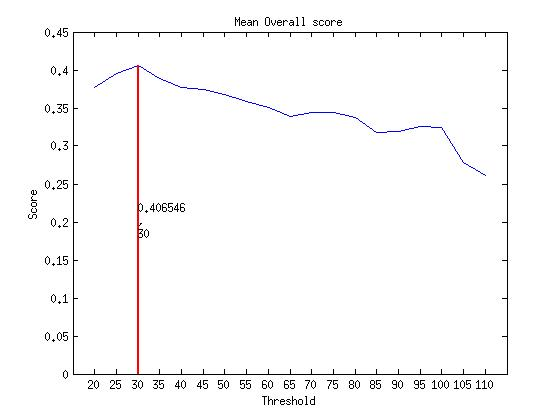
\includegraphics[scale=0.4]{../Drawings/OptimalParameters_SBRISK_SBRISK_KNN.jpg}
\caption{The optimal parameters for BRISK0 with 2-NN}
\label{fig:BRISK0knnOptimal}
\end{minipage}
\hspace{0.5cm}
\begin{minipage}[b]{0.5\linewidth}
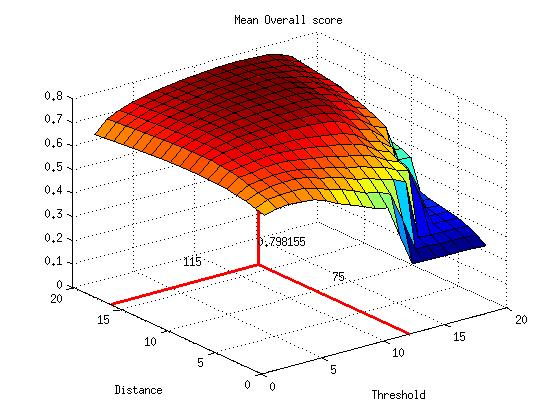
\includegraphics[scale=0.4]{../Drawings/OptimalParameters_SBRISK_SBRISK_hamming.jpg}
\caption{The optimal parameters for BRISK0 with Hamming Distance}
\label{fig:BRISK0hammingOptimal}
\end{minipage}
\begin{minipage}[b]{0.5\linewidth}
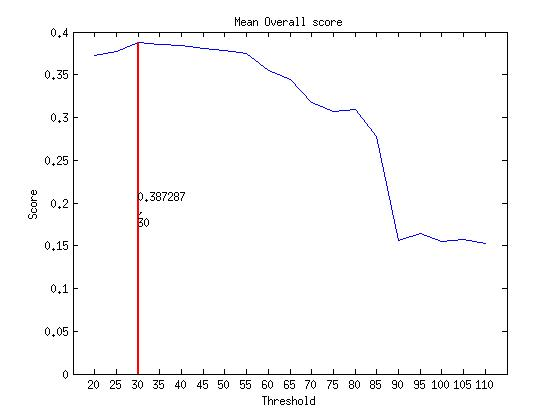
\includegraphics[scale=0.4]{../Drawings/OptimalParameters_BRISK4_BRISK4_KNN.jpg}
\caption{The optimal parameters for BRISK with 2-NN Distance}
\label{fig:BRISKknnOptimal}
\end{minipage}
\begin{minipage}[b]{0.5\linewidth}
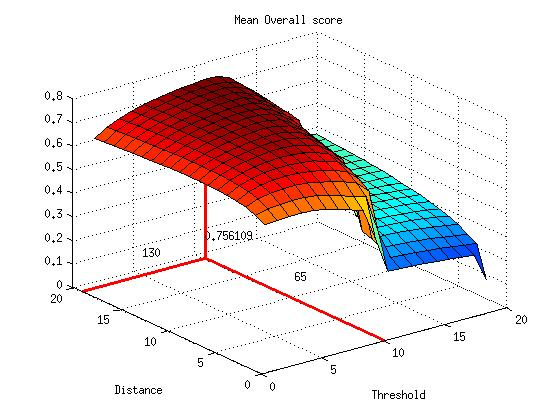
\includegraphics[scale=0.4]{../Drawings/OptimalParameters_BRISK4_BRISK4_Hamming.jpg}
\caption{The optimal parameters for BRISK with Hamming Distance}
\label{fig:BRISKhammingOptimal}
\end{minipage}
\end{figure}

\begin{figure}
\begin{minipage}[b]{0.5\linewidth}
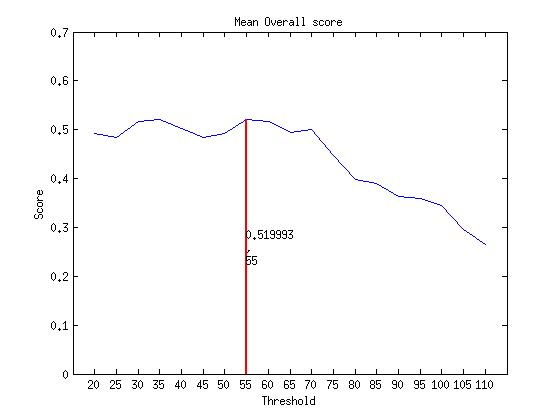
\includegraphics[scale=0.4]{../Drawings/OptimalParameters_SBRISK_SURF2D_KNN.jpg}
\caption{The optimal parameters for BRISK0 SURF2D with 2-NN}
\label{fig:BRISK0surfknnOptimal}
\end{minipage}
\hspace{0.5cm}
\begin{minipage}[b]{0.5\linewidth}
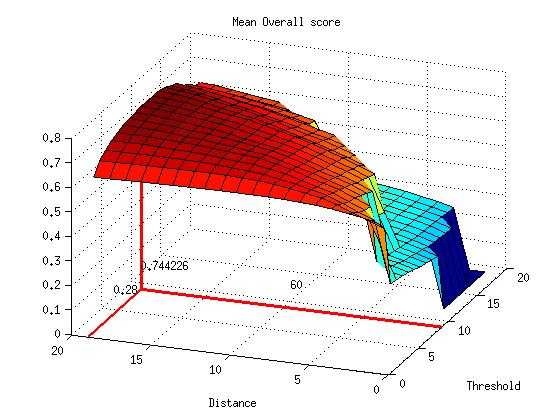
\includegraphics[scale=0.4]{../Drawings/OptimalParameters_SBRISK_SURF2D_Hamming.jpg}
\caption{The optimal parameters for BRISK0 SURF2D with Hamming Distance}
\label{fig:BRISK0surfHammingOptimal}
\end{minipage}
\begin{minipage}[b]{0.5\linewidth}
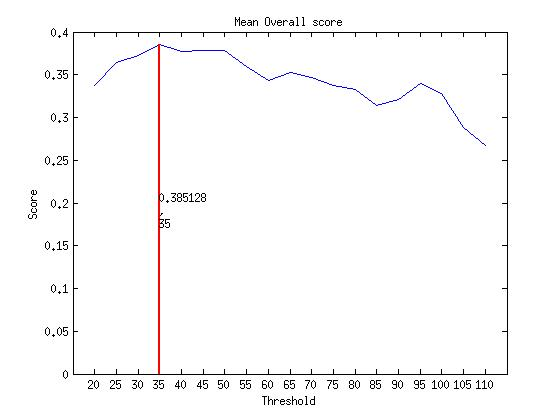
\includegraphics[scale=0.4]{../Drawings/OptimalParameters_SBRISK_UBRISK_KNN.jpg}
\caption{The optimal parameters for BRISK0 - U-BRISK with 2-NN Distance}
\label{fig:BRISK0UBRISKknnOptimal}
\end{minipage}
\begin{minipage}[b]{0.5\linewidth}
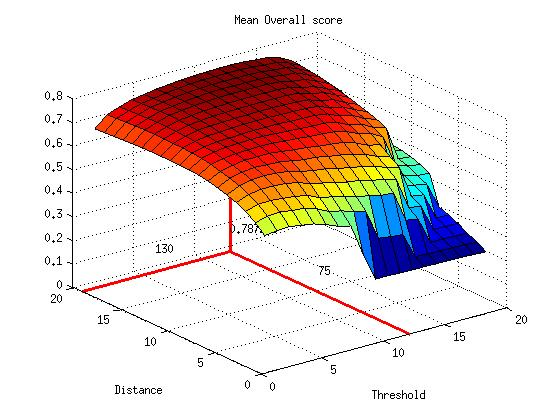
\includegraphics[scale=0.4]{../Drawings/OptimalParameters_SBRISK_UBRISK_Hamming.jpg}
\caption{The optimal parameters for BRISK0 - U-BRISK with Hamming Distance}
\label{fig:BRISK0UBRISKHammingOptimal}
\end{minipage}
\end{figure}



After performing the experiments a set of optimal parameters were generated. The parameter settings are shown in \tabref{tab:knnStatistics} and \tabref{tab:hammingStatistics} respectively. For the 2-NN tests, only the Minimum Interest Point Detection Threshold (MIPDT) parameter was varied in the range $20 \rightarrow 115$ in increments of $5$. For the hamming/euclidean distance tests, both the MIPDT and the maximum hamming/euclidean distance threshold parameters were varied. The MIPDT was varied in the same range as the 2-NN tests. The hamming distance is varied from $40 \rightarrow 135$ in increments of $5$ whereas the euclidean distance is varied from $0.1 \rightarrow 0.28$ in increments of $0.1$. \\



\begin{table}
\caption{The optimal thresholds for the 2-NN feature extraction algorithms}
\footnotesize
\begin{tabular}{|c|c|c|c|c|c|c|c|c|}
\hline 
Detector & Extractor & Matcher & k1 & k2 & k3 & k4 & $MIPDT_{MPS}$ & $MIPDT_{CPS}$\tabularnewline
\hline 
\hline 
S-BRISK & S-BRISK & 2-NN & 0.6 & 0.4 & 0.4 & 0.6 & 46.25 & 30\tabularnewline
\hline 
BRISK4 & BRISK4 & 2-NN & 0.6 & 0.4 & 0.4 & 0.6 & 51.25 & 30\tabularnewline
\hline 
BRISK0 & SURF2D & 2-NN & 0.6 & 0.4 & 0.4 & 0.6 & 43.75 & 30\tabularnewline
\hline 
BRISK0 & UBRISK & 2-NN & 0.6 & 0.4 & 0.4 & 0.6 & 55 & 35\tabularnewline
\hline 
\end{tabular}
\label{tab:knnStatistics}
\end{table}

\begin{table}
\caption{The optimal thresholds for the Hamming/Euclidean distance feature extraction algorithms}
\footnotesize
\begin{tabular}{|c|c|c|c|c|c|c|c|c|c|c|}
\hline 
Detector & Extractor & Matcher & k1 & k2 & k3 & k4 & $MIPDT_{MPS}$ & $MAHD_{MPS}/MAED_{MPS}$ & $MIPDT_{CPS}$ & $MAHD_{CPS}/MAED_{CPS}$\tabularnewline
\hline 
\hline 
S-BRISK & S-BRISK & Radius & 0.6 & 0.4 & 0.4 & 0.6 & 77.5 & 107.5 & 75 & 115\tabularnewline
\hline 
BRISK4 & BRISK4 & Radius & 0.6 & 0.4 & 0.4 & 0.6 & 80 & 120 & 65 & 130\tabularnewline
\hline 
BRISK0 & SURF2D & Radius & 0.6 & 0.4 & 0.4 & 0.6 & 65 & 0.28 & 60 & 0.28\tabularnewline
\hline 
BRISK0 & UBRISK & Radius & 0.6 & 0.4 & 0.4 & 0.6 & 75 & 121.25 & 75 & 130\tabularnewline
\hline 
\end{tabular}
\label{tab:hammingStatistics}
\end{table}

\subsubsection{Matching Score}
\label{sec:matchingScore}
As mentioned in \secref{sec:matching}, in the case of 2D SURF, interest point pairs can be matched based on the euclidean distance between the feature vectors representing the interest points. Similarly, in the case of BRISK, interest points can be matched based on the hamming distance between the feature vectors. In both cases, taking the inverse distance can produce a Matching Score (MS) as shown in \eqnref{eqn:inverseDistance}. Here, $ip_1, ip_2$ represent the pair of interest points being compared and $D$ is the hamming/euclidean distance between the interest points' feature descriptors. The smaller the distance between feature descriptors, the more similar the interest points become resulting in a high matching score and vice versa. In order to determine the Image Matching Score (IMS) between a pair of images, all of the individual MS values are summed together for each of the interest points as seen in \eqnref{eqn:ims}. Here, $i_1, i_2$ represent the images. \\

\begin{equation}
MS_{ip1, ip2} = \frac{1}{D_{ip1, ip2}}
\label{eqn:inverseDistance}
\end{equation}

\begin{equation}
IMS_{i1, i2} = \sum_{ip1, ip2} MS_{ip1, ip2}
\label{eqn:ims}
\end{equation}

In order to determine whether or not this score is a good metric for classifying whether images match or not, an experiment was performed. The experiment involves utilising the images from the datasets in \tabref{table:overlap} to computed matching scores for pairs of overlapping images and pairs of non-overlapping images respectively. It was expected that the matching score for the overlapping images would be larger than that of the non-overlapping images. The BRISK-based feature extraction algorithms utilised for this experiment include BRISK0, BRISK, BRISK0-SURF2D and BRISK0- UBRISK. The matching technique utilised was either 2-Nearest Neighbors (2-NN) or radius matching depending on the feature extraction algorithm.\\

The mean matching scores for $1421$ overlapping images and $2808$ non-overlapping images are shown in \tabref{tab:matchingScoreCompare}. As can be seen in the table, matching scores for overlapping images are at least an order of magnitude larger than matching scores for non-overlapping images. This indicates that \eqnref{eqn:ims} can be utilised as a means to classify whether or not a match has occurred between a pair of images. This score is one of the criterion that has been used to determine the overall performance of each of the feature extraction algorithms and is detailed in \secref{sec:overallPerformance}.\\

\begin{table}
\caption{The matching scores for each of the BRISK-based feature extraction techniques. This is for overlapping and non-overlapping images respectively}
\begin{tabular}{|c|c|c|}
\hline 
Method & Overlapping Score & Non-overlapping Score\tabularnewline
\hline 
\hline 
 & \multicolumn{2}{c}{2-NN}\tabularnewline
\hline 
BRISK0 & 0.213 & 0.002\tabularnewline
\hline 
BRISK4 & 0.167 & 0.002\tabularnewline
\hline 
BRISK0- SURF2D & 66.62 & 3.52\tabularnewline
\hline 
UBRISK & 0.177 & 0.001\tabularnewline
\hline 
 & \multicolumn{2}{c}{Radius Matching}\tabularnewline
\hline 
BRISK0 & 0.22 & 0.02\tabularnewline
\hline 
BRISK4 & 0.21 & 0.01\tabularnewline
\hline 
BRISK0- SURF2D & 50.16 & 3.15\tabularnewline
\hline 
UBRISK & 0.20 & 0.01\tabularnewline
\hline 
\end{tabular}
\label{tab:matchingScoreCompare}
\end{table}

\subsubsection{2-NN Matching Constraint}
\label{sec:knnMatchingConstraint}
In order to verify the 2-NN matching constraint and determine the optimum threshold, a number of tests were developed and implemented on the four main feature extraction techniques, namely BRISK0, BRISK, UBRISK and BRISK0-2D SURF. In order to generate invalid matches, images with no overlap were compared, and any matches found during the comparison were flagged as invalid matches. This was performed on $2808$ non-overlapping image pairs. To generate the valid matches, $108$ identical images were compared and all matches found between these images were flagged as valid matches. In both cases, 2-NN matching was performed generating two matches for every interest point. The ratio of the first and second 2-NN neighbor was then computed for both valid and invalid matches and the mean ratio was subsequently generated. The results are shown in \tabref{tab:knnCriterion} for each of the four methods. As can be seen in the table, invalid matches have a mean ratio which is over $0.9$. Valid matches have a ratio which is approximately zero. This illustrates a significant difference between the first and second 2-NN for valid and invalid matches. Based on this data, all matches whose 2-NN ratio is below $0.7$ are considered valid matches whereas all matches above $0.7$ are considered to be invalid matches. This value has been chosen in order to ensure that the majority of 2-NN invalid matches are rejected. Since the largest standard deviation is $8.8\%$ of the total 2-NN ratio value, a value well below $0.9$ has been selected. Graphs of the 2-NN ratio for both the BRISK0 - U-BRISK method and BRISK0-BRISK0 method are shown in \figref{fig:b0ubknnratio} and \figref{fig:b0knnratio} respectively. \\

\begin{figure}[h!]
\begin{minipage}[b]{0.5\linewidth}
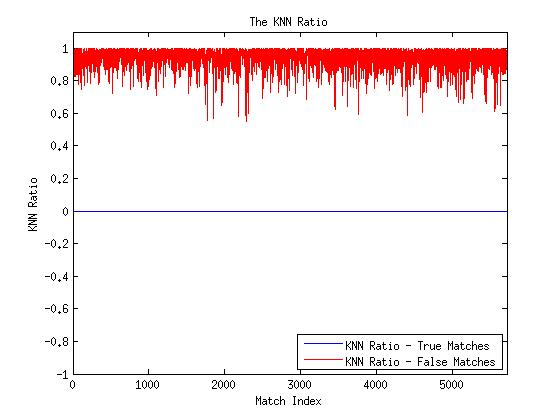
\includegraphics[scale=0.5]{../Drawings/KNNRatio_SBRISK_UBRISK_20_60.jpg}
\caption{The 2-NN ratio for non-overlapping and overlapping images respectively using the BRISK0 - UBRISK method}
\label{fig:b0ubknnratio}
\end{minipage}
\hspace{0.5cm}
\begin{minipage}[b]{0.5\linewidth}
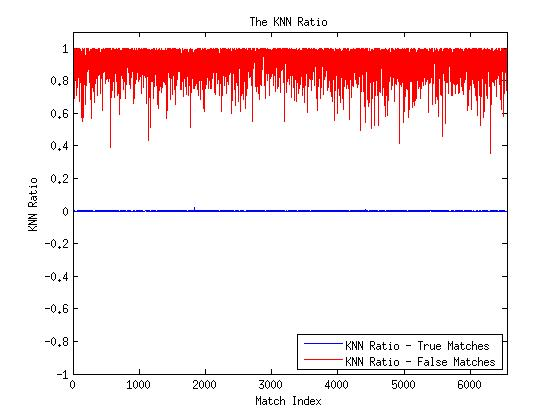
\includegraphics[scale=0.5]{../Drawings/KNNRatio_SBRISK_SURF2D_20_60.jpg}
\caption{The 2-NN ratio for non-overlapping and overlapping images respectively using the BRISK0 method}
\label{fig:b0knnratio}
\end{minipage}
\end{figure}

In addition to this, the mean distance between the first and second 2-NN for each method have been computed. It has been found that there is a significant difference between the distances for valid and invalid matches respectively. The mean distance could also be used as a global threshold but this is not generic and some feature descriptors may be more discriminatory than others \cite{Lowe2004}. This is evident in the case of BRISK0-2D SURF as the standard deviation is $68\%$ of the total value indicating a huge amount of fluctuation about the mean. Thus the 2-NN ratio is a more useful constraint in this scenario.\\

\begin{table}
\caption{The 2-NN Ratios}
\footnotesize
\begin{tabular}{|c|c|c|c|c|c|}
\hline 
Method & Match Type & Mean 2-NN Ratio & Std Deviation & Mean Distance between 2-NN neighbors & Std Deviation\tabularnewline
\hline 
\hline 
BRISK0 & Invalid Matches & 0.94 & 0.06 & 7.45 & 7.58\tabularnewline
\hline 
 & Valid Matches & 0 & 0 & 97.66 & 37.97\tabularnewline
\hline 
BRISK & Invalid Matches & 0.93 & 0.06 & 7.93 & 7.91\tabularnewline
\hline 
 & Valid Matches & 0 & 0 & 86.47 & 42.78\tabularnewline
\hline 
BRISK0 - UBRISK & Invalid Matches & 0.94 & 0.05 & 7.78 & 7.58\tabularnewline
\hline 
 & Valid Matches & 0 & 0 & 100.70 & 40.21\tabularnewline
\hline 
BRISK0 SURF2D & Invalid Matches & 0.90 & 0.08 & 0.03 & 0.03\tabularnewline
\hline 
 & Valid Matches & 0.0004 & 0.0008 & 0.25 & 0.18\tabularnewline
\hline 
SURF 1D & Invalid Matches &  &  &  & \tabularnewline
\hline 
 & Valid Matches &  &  &  & \tabularnewline
\hline 
\end{tabular}
\label{tab:knnCriterion}
\end{table}




\subsubsection{Interest Point Matching Properties}
\label{sec:keypointMatching}
It is also important to determine whether or not interest points corresponding to a valid match have different properties compared to interest points corresponding to an invalid match. This could be useful in generating new constraints that can effectively remove invalid matches. Three criteria were analysed, namely the angle $\alpha_i$, size $S_i$ and response $R_i$ of each pair of matched interest points. The subscript $i|i={1,2}$ refers to the image number of the interest point being evaluated.\\

In order to generate useful statistics for this experiment, the angle, size and response of each of the interest points in image $1$ are subtracted from the angle, size and response of the corresponding matched interest points in image $2$. All of these differences are then summed together for all the matched interest points in each pair of images. The mean is subsequently computed. This results in the mean differences $\bar{d\alpha}, \bar{dS}$ and $\bar{dR}$ as shown in \eqnref{eqn:differenceProperties} respectively. The angle, response and size mean differences as well as the standard deviation for each of these differences are calculated using $40$ overlapping image pairs from all four datasets.\\ \\

\begin{eqnarray}
\bar{d\alpha} &=& \frac{\sum_{j=1}^N (\alpha_1^j - \alpha_2^j)}{N}\\
\bar{dS} &=& \frac{\sum_{j=1}^N (S_1^j - S_2^j)}{N}\\
\bar{dR} &=& \frac{\sum_{j=1}^N (R_1^j - R_2^j)}{N}
\label{eqn:differenceProperties}
\end{eqnarray}

%The mean distance between 
In order to determine whether or not matches in images are valid, the two matching constraints discussed in \secref{sec:validation} have been utilised, namely, the angle and distance constraint and the the 2-NN ratio constraint. Utilising these constraints, overlapping image pairs were compared using the four feature extraction algorithms. The MPS values from \tabref{tab:knnStatistics} have been used to perform these experiements. \\

The interest points corresponding to valid and invalid matches in each of the images respectively were tabulated. Invalid matches due to the angle and distance constraints are tabulated separately from the invalid matches due to the 2-NN ratio constraint. The mean angle, response and size differences from the image pairs as well as the corresponding standard deviations are shown in \tabref{tab:keypointProperties}.\\

It is important to note that BRISK0 - U-BRISK and BRISK0 - 2D SURF do not output interest point angles. Thus these methods cannot be compared using the angle criterion. In addition to this, since BRISK0 only detects interest points in a single scale space, the size of the detected interest point scale remains the same. Therefore, this criterion is not used as a means of comparison for all of the BRISK0-based methods.\\

One of the more significant observations is the mean response difference $\bar{dR}$. The difference $dR$ is much smaller for valid matches compared to invalid matches over all four methods. This seems to indicate that the response of valid interest points is generally very similar.\\

In addition to this, BRISK0 and BRISK exhibit a large difference in interest point angles $\bar{d\alpha}$ for invalid matches and a much smaller difference for valid matches. \\

Finally, difference in detected scales $\bar{dS}$ has been found to be much smaller for valid matches than for invalid matches. As mentioned previously, this statistic is only valid for BRISK based detectors (BRISK0 is not included among these detectors).\\

Therefore, it may be possible to utilise these properties in order to further detect and remove invalid matches in images. This is a recommendation for further work on this topic.\\

%The keypoints in image A were subtracted from the keypoints in image B.

\begin{table}


\caption{The properties of valid and invalid interest point matches}


\begin{tabular}{|c|c|c|c|c|c|r@{\extracolsep{0pt}.}l|}
\hline 
Property & \multicolumn{7}{c}{Invalid Matches due to Angle Constraint}\tabularnewline
\hline 
\hline 
Method & $\bar{d\alpha}$ & $\bar{d\alpha}$Std & $\bar{dR}$ & $\bar{dR}$Std & $\bar{dS}$ & \multicolumn{2}{c|}{$\bar{dS}$Std}\tabularnewline
\hline 
BRISK0 & 20.28 & 6.680 & 0.5400 & 1.070 & 0 & \multicolumn{2}{c|}{0}\tabularnewline
\hline 
BRISK & 6.98 & 1.47 & 6.31 & 2.88 & 0.300 & 2&54\tabularnewline
\hline 
BRISK0 - SURF2D & 0 & 0 & 0.4300 & 0.8900 & 0 & \multicolumn{2}{c|}{0}\tabularnewline
\hline 
UBRISK & 0 & 0 & 0.13 & 2.060 & 0 & \multicolumn{2}{c|}{0}\tabularnewline
\hline 
 & \multicolumn{7}{c}{Invalid Matches due to 2-NN Ratio Constraint}\tabularnewline
\hline 
BRISK0 & 4.280 & 0.8700 & 6.810 & 1.980 & 0 & \multicolumn{2}{c|}{0}\tabularnewline
\hline 
BRISK & 3.24 & 4.84 & 2.43 & 1.03 & 3.02 & 4&58\tabularnewline
\hline 
BRISK0 - SURF2D & 0 & 0 & 2.370 & 1.700 & 0 & \multicolumn{2}{c|}{0}\tabularnewline
\hline 
UBRISK & 0 & 0 & 4.610 & 1.710 & 0 & \multicolumn{2}{c|}{0}\tabularnewline
\hline 
 & \multicolumn{7}{c}{Valid Matches}\tabularnewline
\hline 
BRISK0 & 0.6600 & 0.5200 & 0.08000 & 0.1000 & 0 & \multicolumn{2}{c|}{0}\tabularnewline
\hline 
BRISK & 1.20 & 0.310 & -0.860 & 0.0500 & -0.0900 & 0&410\tabularnewline
\hline 
BRISK0 - SURF2D & 0 & 0 & 0.2900 & 0.2700 & 0 & \multicolumn{2}{c|}{0}\tabularnewline
\hline 
UBRISK & 0 & 0 & -0.11 & -0.44 & 0 & \multicolumn{2}{c|}{0}\tabularnewline
\hline 
\end{tabular}
\label{tab:keypointProperties}
\end{table}

%A picture of the graph for each method containing the optimal parameters


\subsection{Overall Performance}
\label{sec:overallPerformance}

%These tables will be needed when describing why some methods perform better than others. This will therefore be included in the overall performance section

%This data was generated by considering overlapping and non-overlapping images
%The valid matches and invalid matches should differ between the matching and overlapping sets respectively.

\begin{table}
\caption{The matching and interest point statistics for each of the various methods using the 2-NN matching criterion}
\begin{tabular}{|c|c|c|c|c|}
\hline 
Method (2-NN) & \multicolumn{4}{c}{Overlapping images}\tabularnewline
\hline 
\hline 
 & Total Matches & Valid Matches & Invalid Matches & Mean Num Interest Points\tabularnewline
\hline 
BRISK0  & 175.560 & 15.42 & 160.14 & 77.43000\tabularnewline
\hline 
BRISK4 & 175.6300 & 13.23000 & 162.4100 & 73.70000\tabularnewline
\hline 
BRISK0-SURF2D  & 218.8800 & 19.01000 & 199.8600 & 97.88000\tabularnewline
\hline 
BRISK0 - UBRISK & 135.7600 & 16.14000 & 119.6200 & 59.38000\tabularnewline
\hline 
 & \multicolumn{4}{c}{Non-overlapping images}\tabularnewline
\hline 
 &  &  &  & \tabularnewline
\hline 
BRISK0  & 72.260 & 0.25000 & 72.010 & 77.430\tabularnewline
\hline 
BRISK4  & 69.930 & 0.28000 & 69.640 & 73.700\tabularnewline
\hline 
BRISK0-SURF2D & 98.700 & 1.3900 & 97.310 & 97.880\tabularnewline
\hline 
BRISK0 - UBRISK & 54.560 & 0.22000 & 54.340 & 59.380\tabularnewline
\hline 
\end{tabular}
\label{tab:keypointsMatchesKNN}
\end{table}

\begin{table}
\caption{The matching and interest point statistics for each of the various methods using the Radius Matching criterion}
\begin{tabular}{|c|c|c|c|c|}
\hline 
Method (Radius Matching) & Total Matches & Valid Matches & Invalid Matches & Mean Num Keypoints\tabularnewline
\hline 
\hline 
 & \multicolumn{4}{c}{Overlapping images}\tabularnewline
\hline 
BRISK0  & 70.770 & 39.980 & 30.790 & 32.420\tabularnewline
\hline 
BRISK4  & 91.380 & 57.510 & 33.870 & 31.560\tabularnewline
\hline 
BRISK0-SURF2D & 19.530 & 12.050 & 7.4800 & 51.940\tabularnewline
\hline 
BRISK0 - UBRISK & 40.120 & 26.930 & 13.190 & 33.530\tabularnewline
\hline 
 & \multicolumn{4}{c}{Non-overlapping images}\tabularnewline
\hline 
BRISK0 & 11.150 & 4.9600 & 6.1900 & 32.420\tabularnewline
\hline 
BRISK4 & 5.6300 & 2.3900 & 3.2500 & 31.560\tabularnewline
\hline 
BRISK0-SURF2D & 2.6800 & 0.90000 & 1.7800 & 51.940\tabularnewline
\hline 
BRISK0 - UBRISK & 3.9700 & 1.8500 & 2.1200 & 33.530\tabularnewline
\hline 
\end{tabular}
\label{tab:keypointsMatchesHamming}
\end{table}

In order to determine the detector with the best overall performance, the following test procedure was performed. The optimal thresholds (both MPS and CPS) for both the 2-NN and Radius Matching based feature extraction algorithms were used as the parameter settings for these algorithms. Each algorithm was then run on a set of $1421$ overlapping image pairs and $2808$ non-overlapping image pairs. The average times corresponding to each section of the algorithm were recorded and the results are shown in \tabref{tab:overallknn} and \tabref{tab:overallhammingeuclidean} respectively. The detection time is defined as the amount of time required to detect all of the interest points in a single detector module. The extraction time is the time taken to compute the descriptors of the detected interest points for a single descriptor module. The matching time is the time taken to match the interest points for a single pair of images. The verification time is the time taken to detect and remove invalid invalid interest points. Finally the overall time is the summation of these times as well as the time to process and extract the image from the robot. \\

As can be seen in the tables, the algorithm producing the marginally best matching performance using 2-NN matching is BRISK0 - 2D SURF with an Area Under the ROC Curve (AUC) of $93.799\%$. However, this algorithm comes at a high computational cost as it is computing the euclidean distance between $64$ dimensional feature descriptors for every detected interest point match. This fact is evident as the detection time for this method is almost twice as slow as the other methods regardless of the matching technique implemented.\\

In terms of speed, the best performing 2-NN feature extraction algorithm is BRISK0 - U-BRISK with a best overall time of $9.43 ms$. This is expected since a number of constraints have been relaxed. These include the single scale constraint as well as removing rotation invariance as mentioned in \secref{sec:brisk0}. These constraints have been implemented in order to maximise computational efficiency and therefore satisfy the computational requirements of the Nao robot. This method therefore has the fastest extraction time of $1.95 ms$ as the sampling pattern is not rotated in this variation of the BRISK technique.\\

The BRISK4 technique has a large feature detection time. This is is because the method is calculating features across multiple scales. A 3D interpolation is also performed as mentioned previously in order to generate continuous scale refinements. This is a time consuming operation and results in the drop in performance. It should also be noted that the BRISK4 technique does not have a large AUC. In the 2-NN Matching tests, its largest AUC is $90.76\%$ and in the Radius Matching tests, its largest AUC is $80.78\%$. This is partially due to the fact that the BRISK4 algorithm detects interest points by performing a non-maximal suppression over scale space. This filters out more interest points as these points have to fulfil a more demanding constraint than that imposed in the BRISK0 implementation. The BRISK0 implementation simply detects interest points if they are not suppressed in a single scale dimensional.\\

The 1D SURF technique seems to struggle in this environment as it only manages to attain an AUC of $69.21\%$. It is possible that since there is a small amount of variation in the scene, there may be a problem identifying features since the single row of pixels may have a large number of similar pixel values. This performance improves when there is more variation in the images and will be presented in \secref{sec:additionalDataset}. However, in terms of overall speed, this method is among the fastest with an overall time of $13.19$ seconds. Most notably, the detection and extraction times are an order of magnitude faster than the BRISK-based techniques.\\

The algorithm with the best general performance is BRISK0 - U-BRISK using Radius Matching and the MPS parameter values. At its best, this algorithm performs the entire feature extraction routine in $9.43 ms$ which is significantly faster than the other tested methods. In addition, the matching performance is $90.38\%$ which is acceptable performance for this application.\\

\begin{table}
\centering
\caption{The performance statistics of 2-NN feature extraction algorithms}
\footnotesize
\begin{tabular}{|c|c|c|c|c|c|c|c|}
\hline 
\textbf{Method (2-KNN)} & Parameter & \% AUC & Detection(ms) & Extraction(ms) & Matching(ms) & Verification(ms) & Overall(ms)\tabularnewline
\hline 
\hline 
BRISK0 & MPS & 90.429 & 3.4840 & 6.0540 & 1.7070 & 0.029000 & 15.271\tabularnewline
\hline 
BRISK4 & MPS & 88.084 & 10.882 & 5.8820 & 1.5710 & 0.029000 & 22.422\tabularnewline
\hline 
BRISK0 - SURF2D & MPS & 93.586 & 3.6230 & 12.016 & 0.57800 & 0.039000 & 20.304\tabularnewline
\hline 
\textbf{BRISK0 - U-BRISK} & \textbf{MPS} & \textbf{87.830} & \textbf{3.3320} & \textbf{2.5950} & \textbf{1.0580} & \textbf{0.024000} & \textbf{11.005}\tabularnewline
\hline 
BRISK0 & CPS & 93.064 & 4.1300 & 11.108 & 6.4990 & 0.053000 & 25.810\tabularnewline
\hline 
BRISK4 & CPS & 90.768 & 15.842 & 10.970 & 6.7440 & 0.057000 & 37.662\tabularnewline
\hline 
BRISK0 - SURF2D & CPS & 93.799 & 4.2050 & 20.799 & 1.4910 & 0.067000 & 30.628\tabularnewline
\hline 
BRISK0 - U-BRISK & CPS & 90.350 & 3.8320 & 4.0510 & 3.7750 & 0.042000 & 15.709\tabularnewline
\hline 
\textbf{SURF 1D} & \textbf{Given} & \textbf{69.208} & \textbf{0.27000} & \textbf{0.13400} & \textbf{0.24400} & \textbf{0.028000} & \textbf{13.185}\tabularnewline
\hline 
\end{tabular}
\label{tab:overallknn}
\end{table}

\begin{table}
\centering
\caption{The performance statistics of Radius Matching feature extraction algorithms}
\footnotesize
\begin{tabular}{|c|c|c|c|c|c|c|c|}
\hline 
Method & Parameters & \% AUC & Detection(ms) & Extraction(ms) & Matching(ms) & Verification(ms) & Overall(ms)\tabularnewline
\hline 
\hline 
BRISK0 & MPS & 82.908 & 3.0800 & 3.2180 & 0.35200 & 0.016000 & 10.717\tabularnewline
\hline 
BRISK4 & MPS & 76.616 & 8.4920 & 3.3550 & 0.32200 & 0.016000 & 16.259\tabularnewline
\hline 
BRISK0-SURF2D & MPS & 86.347 & 3.2310 & 7.2990 & 0.26500 & 0.0090000 & 14.865\tabularnewline
\hline 
\textbf{BRISK0-UBRISK} & MPS & \textbf{90.378} & \textbf{3.0970} & \textbf{1.9530} & \textbf{0.36000} & \textbf{0.010000} & \textbf{9.4310}\tabularnewline
\hline 
BRISK0 & CPS & 83.177 & 3.1130 & 3.3270 & 0.38300 & 0.021000 & 10.860\tabularnewline
\hline 
BRISK4 & CPS & 80.778 & 9.5310 & 4.3610 & 0.67600 & 0.041000 & 18.694\tabularnewline
\hline 
BRISK0-SURF2D & CPS & 86.818 & 3.2910 & 8.3150 & 0.31200 & 0.011000 & 15.969\tabularnewline
\hline 
BRISK0-UBRISK & CPS & 89.922 & 3.1140 & 1.9970 & 0.36700 & 0.012000 & 9.5030\tabularnewline
\hline 
\textbf{SURF 1D} & \textbf{Given} & \textbf{69.208} & \textbf{0.27000} & \textbf{0.13400} & \textbf{0.24400} & \textbf{0.028000} & \textbf{13.185}\tabularnewline
\hline 
\end{tabular}
\label{tab:overallhammingeuclidean}
\end{table}

The ROC curves generated have been generated for each of the four methods. These curves have been generated by utilising the overlapping and non-overlapping images respectively. Overlapping images generate the True Positive (TP) matches. This is performed by varying the matching score threshold in a range from the maximum matching score in the dataset to $0$.  All overlapping image pairs with a larger matching score than the threshold are classified as a match and all overlapping image pairs below the matching score are classified as a non-match. The False Positives (FP) are generated from the non-overlapping image pairs. Again, the matching score threshold is varied and all non-overlapping image pairs above the threshold are defined as a match and vice versa. If a non-overlapping image is defined as a match, then it is a FP. The ROC curves for the four methods are shown in \figref{fig:compareHamming} to \figref{fig:compareKNNConsistent} respectively.\\

\figref{fig:compareHamming} and \figref{fig:compareHammingConsistent} shows the ROC curves for the four methods using Radius Matching and MPS and CPS parameter values respectively defined in \secref{sec:optimalParameters}. \figref{fig:compareKNN} shows the ROC curves for 2-NN and using the MPS. Finally, \figref{fig:compareKNNConsistent} shows the 2-NN matching ROC curves using the CPS.\\

\begin{figure}[h!]
\begin{minipage}[b]{0.5\linewidth}
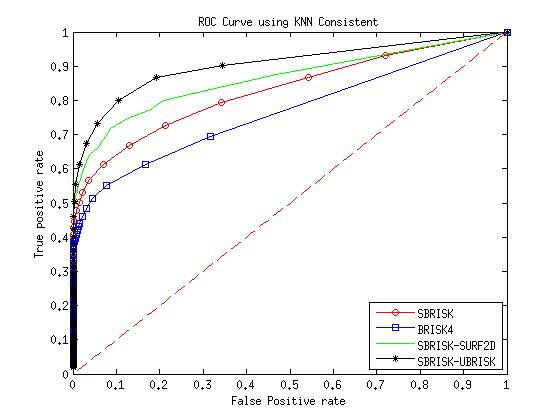
\includegraphics[scale=0.4]{../Drawings/ROC_General_Hamming.jpg}
\caption{A comparison of the ROC curves for the Robocup datasets using Radius Matching and MPS values}
\label{fig:compareHamming}
\end{minipage}
\hspace{0.5cm}
\begin{minipage}[b]{0.5\linewidth}
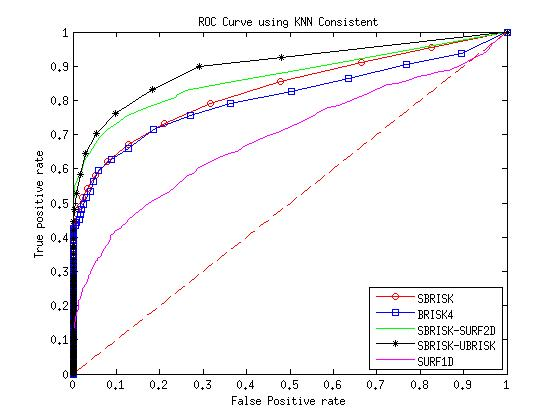
\includegraphics[scale=0.4]{../Drawings/ROC_General_Hamming_Consistent.jpg}
\caption{A comparison of the ROC curves for the Robocup datasets using Radius Matching and CPS values}
\label{fig:compareHammingConsistent}
\end{minipage}
\begin{minipage}[b]{0.5\linewidth}
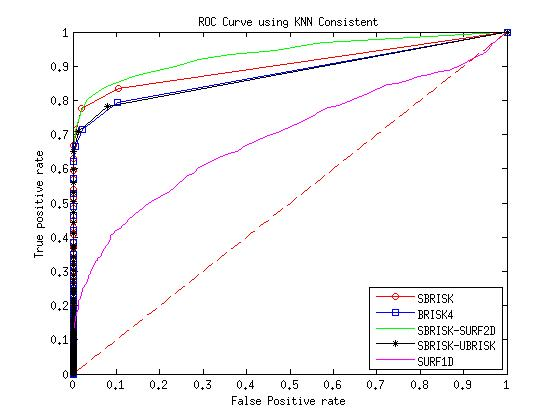
\includegraphics[scale=0.4]{../Drawings/ROC_General_KNN.jpg}
\caption{A comparison of the ROC curves for the Robocup datasets using 2-NN for matching and MPS values}
\label{fig:compareKNN}
\end{minipage}
\begin{minipage}[b]{0.5\linewidth}
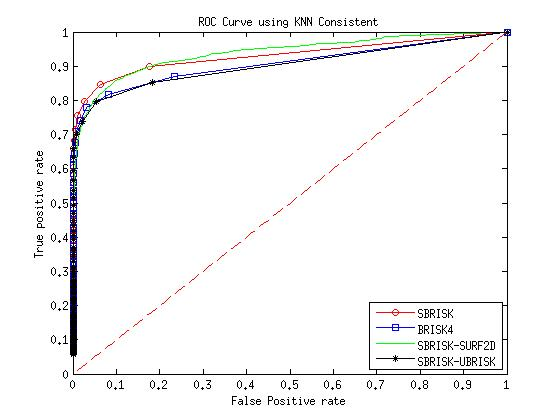
\includegraphics[scale=0.4]{../Drawings/ROC_General_KNN_Consistent.jpg}
\caption{A comparison of the ROC curves for the Robocup datasets using 2-NN for matching and CPS values}
\label{fig:compareKNNConsistent}
\end{minipage}
\end{figure}

Based on the above statistics, it seems that the BRISK0- U-BRISK algorithm using the Radius Matching technique and MPS values seems to produce the best performance, and should therefore be implemented on the robot. Since it can perform image processing and feature extraction in approximately $11 ms$, it should be possible to use this method in real-time on the robot to perform the matching routine and ultimately help the robot disambiguate its position on the field.\\

\subsection{Performance in Different Environment}
\label{sec:additionalDataset}
In order to verify that the BRISK0 - U-BRISK method has better performance than the other feature extraction algorithms, the algorithms have been tested in different environments. The first environment is a random office and the second environment is a large hall. The random office has been selected in order to add natural light into the scene from a large window that will be presented in \secref{sec:office}. It also has a number of salient features that may improve or inhibit feature extraction performance. The large hall has been chosen such that the resolution of the images are lower since the Nao is observing features at large distances. This environment also many salient features. \\

\subsubsection{Office Environment}
\label{sec:office}
Two datasets have been created from a random office environment. In total $25$ overlapping images from one side of the office correspond to one dataset and a further $25$ overlapping images from another view of the office correspond to a second dataset. These images have been taken at different scales and angles. Typical images from each viewpoint are shown in \figref{fig:dataset5} and \figref{fig:dataset6} respectively.\\


\begin{figure}[h!]
\begin{minipage}[b]{0.5\linewidth}
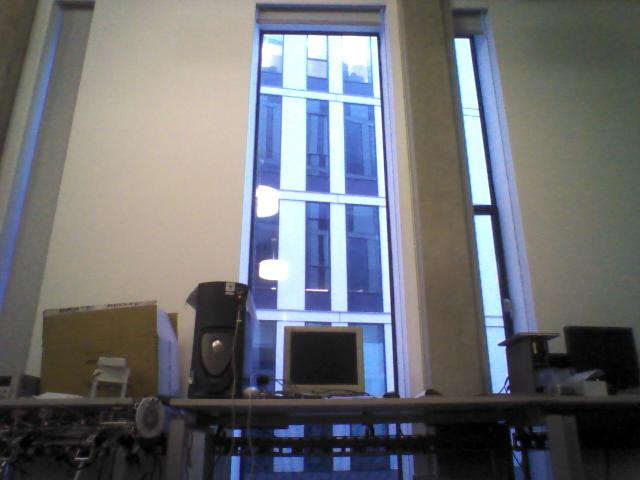
\includegraphics[scale=0.5]{../Drawings/datasetImages/dataset5.jpg}
\caption{The first dataset showing a typical image from one side of the random office environment}
\label{fig:dataset5}
\end{minipage}
\hspace{0.5cm}
\begin{minipage}[b]{0.5\linewidth}
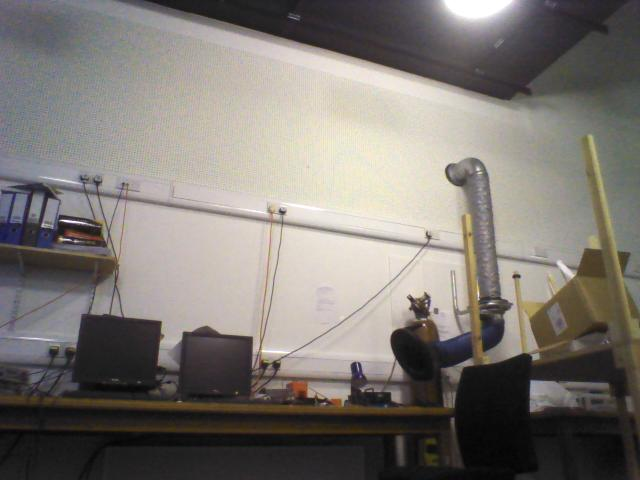
\includegraphics[scale=0.5]{../Drawings/datasetImages/dataset6.jpg}
\caption{The second dataset showing a typical image from one side of the random office environment}
\label{fig:dataset6}
\end{minipage}
\end{figure}

In total $600$ overlapping pairs of images and $600$ non-overlapping pairs of images were generated respectively. Utilising the MPS and CPS parameter values calculated in \secref{sec:overallPerformance}, the feature extraction algorithms were tested on each of the overlapping and non-overlapping image pairs. The feature extraction algorithms were tested using both the 2-NN matching and Radius Matching techniques respectively. The corresponding ROC curves generated from this data are displayed in \figref{fig:compareKnnOffice} to \figref{fig:compareHammingConsistentOffice}. \\

\figref{fig:compareKnnOffice} and \figref{fig:compareHammingOffice} shows the ROC curves that were generated when using the MPS values and 2-NN and Radius Matching respectively. \figref{fig:compareKnnConsistentOffice} and \figref{fig:compareHammingConsistentOffice} have been generated using the CPS values and 2-NN and Radius Matching respectively. As can be seen in the figures, the ROC curves exhibit good matching performance for each of the algorithms. The statistics quantifying the performance are shown in \tabref{tab:rocTimingOfficeKnn} and \tabref{tab:rocTimingOfficeHamming} for 2-NN and Radius Matching respectively. \\

The AUC of the feature extraction algorithms on this dataset is better than on the previous dataset. This may be due to the fact that the new datasets have areas of high contrast between neighboring pixels, such as the window area shown in \figref{fig:dataset5}. Since the BRISK and SURF-based techniques rely on salient differences between neighboring pixel intensities in order to detect interest points, these types of images may create better discrimination for the feature extraction algorithms. This would result in more salient interest points which ultimately enhances matching performance.\\

In addition to this, since the matching score between images is generally much larger for overlapping images compared to non-overlapping images as shown in \secref{sec:matchingScore}, it is expected that a large AUC value will be generated. This is because most of the TP matches will have much higher matching scores than the FP matches. Thus as the matching score threshold is varied, the TP rate will initially be much larger than the FP rate, effectively generating the large AUC value. \\

As can be seen in the table, BRISK0 has the best AUC value of $98.46\%$. However, timing is also a big concern and thus the best overall feature extraction algorithm is again the BRISK0 - U-BRISK combination. It performs a match between two images in the fastest time of $10.45 ms$ in the best case, and has performance comparable to BRISK0.\\  

The 1D SURF implementation has also improved upon its performance as expected due to the large amount of salient features in the dataset images. The algorithm is able to better match the features and subsequently generate a larger AUC value. In addition to this improvement, the algorithm still maintains its speed and produces the fastest feature detection and matching performance. However, the overall timing performance is comparable to BRISK0 - U-BRISK as the intermediate stages such as image processing tend to be slower for the 1D SURF implementation.\\


%The images are also taken in a setting of higher contrast.

%DISCUSS THAT THE HIGHEST TP MATCHING RATE AT WHICH THE FP RATE IS STILL 0, IS A GOOD INDICATOR OF PERFORMANCE.


\begin{figure}[h!]
\begin{minipage}[b]{0.5\linewidth}
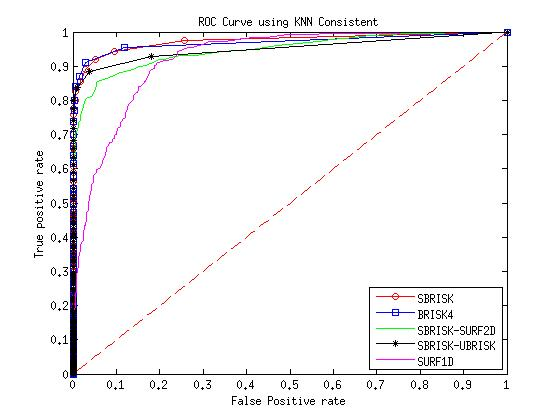
\includegraphics[scale=0.4]{../Drawings/dataset2_ROC_General_KNN.jpg}
\caption{A comparison of the ROC curves in the office environment using the MPS thresholds}
\label{fig:compareKnnOffice}
\end{minipage}
\hspace{0.5cm}
\begin{minipage}[b]{0.5\linewidth}
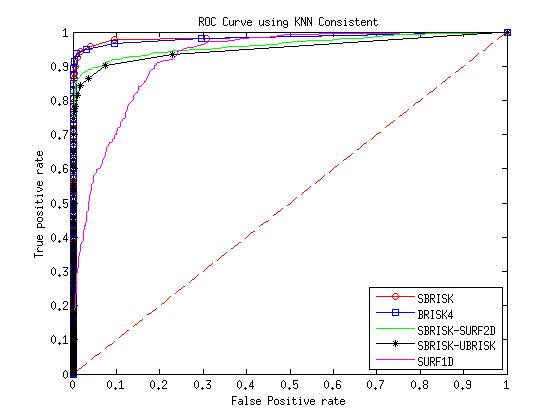
\includegraphics[scale=0.4]{../Drawings/dataset2_ROC_General_KNN_Consistent.jpg}
\caption{A comparison of the ROC curves in the office environment using the CPS thresholds}
\label{fig:compareKnnConsistentOffice}
\end{minipage}
\begin{minipage}[b]{0.5\linewidth}
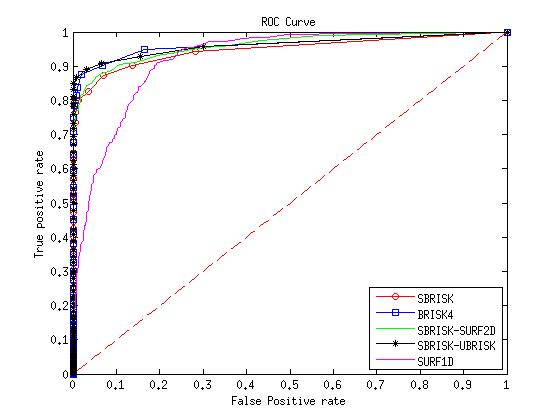
\includegraphics[scale=0.4]{../Drawings/dataset2_ROC_General_Hamming.jpg}
\caption{A comparison of the ROC curves in the office environment using the MPS Hamming/Euclidean distance thresholds}
\label{fig:compareHammingOffice}
\end{minipage}
\hspace{0.5cm}
\begin{minipage}[b]{0.5\linewidth}
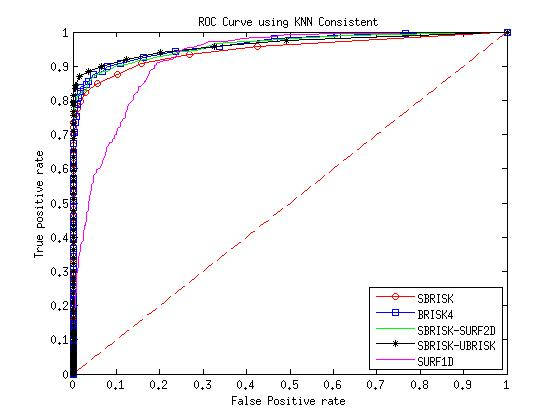
\includegraphics[scale=0.4]{../Drawings/dataset2_ROC_General_Hamming_Consistent.jpg}
\caption{A comparison of the ROC curves in the office environment using the CPS Hamming/Euclidean distance thresholds}
\label{fig:compareHammingConsistentOffice}
\end{minipage}
\end{figure}



\begin{table}
\caption{The AUC and performance statistics for the office environment using
2-NN}
\tiny
\begin{tabular}{|c|c|c|c|c|c|c|c|}
\hline 
\textbf{Method (2-NN)} & \textbf{Parameters} & \textbf{\% AUC} & \textbf{Detection(ms)} & \textbf{Extraction(ms)} & \textbf{Matching(ms)} & \textbf{Verification(ms)} & \textbf{Overall(ms)}\tabularnewline
\hline 
\hline 
BRISK0 & MPS & 97.441 & 3.6950 & 8.1660 & 5.5120 & 0.065000 & 21.838\tabularnewline
\hline 
BRISK4 & MPS & 96.933 & 12.096 & 7.1060 & 5.2520 & 0.072000 & 28.970\tabularnewline
\hline 
BRISK0-SURF2D & MPS & 94.795 & 3.7930 & 17.157 & 1.4970 & 0.083000 & 26.936\tabularnewline
\hline 
\textbf{BRISK0-UBRISK} & MPS & \textbf{95.134} & \textbf{3.4690} & \textbf{3.1120} & \textbf{3.2450} & \textbf{0.052000} & \textbf{14.245}\tabularnewline
\hline 
BRISK0 & CPS & 98.457 & 4.4990 & 14.911 & 17.984 & 0.11200 & 41.889\tabularnewline
\hline 
BRISK4 & CPS & 98.282 & 18.546 & 15.856 & 24.097 & 0.13700 & 63.065\tabularnewline
\hline 
BRISK0-SURF2D & CPS & 96.210 & 4.5200 & 28.129 & 3.6000 & 0.13100 & 40.822\tabularnewline
\hline 
BRISK0-UBRISK & CPS & 95.182 & 4.1490 & 5.2980 & 11.723 & 0.090000 & 25.666\tabularnewline
\hline 
\textbf{SURF 1D} & \textbf{Given} & \textbf{92.333} & \textbf{0.27700} & \textbf{0.19700} & \textbf{0.48300} & \textbf{0.043000} & \textbf{14.144}\tabularnewline
\hline 
\end{tabular}
\label{tab:rocTimingOfficeKnn}
\end{table}

\begin{table}
\caption{The AUC and performance statistics for the office environment using
Hamming/Euclidean distance}
\tiny
\begin{tabular}{|c|c|c|c|c|c|c|c|}
\hline 
\textbf{Method} & \textbf{Parameters} & \textbf{\% AUC} & \textbf{Detection(ms)} & \textbf{Extraction(ms)} & \textbf{Matching(ms)} & \textbf{Verification(ms)} & \textbf{Overall(ms)}\tabularnewline
\hline 
\hline 
BRISK0 & MPS & 94.846 & 3.0940 & 3.4610 & 0.80800 & 0.011000 & 11.710\tabularnewline
\hline 
BRISK4 & MPS & 96.226 & 8.6260 & 3.2650 & 0.84700 & 0.012000 & 17.198\tabularnewline
\hline 
BRISK0-SURF2D & MPS & 96.054 & 3.2550 & 8.4950 & 0.48900 & 0.019000 & 16.626\tabularnewline
\hline 
\textbf{BRISK0-UBRISK} & \textbf{MPS} & \textbf{96.149} & \textbf{3.1250} & \textbf{2.0570} & \textbf{0.88300} & \textbf{0.014000} & \textbf{10.453}\tabularnewline
\hline 
BRISK0 & CPS & 94.697 & 3.1180 & 3.5900 & 0.88900 & 0.014000 & 11.948\tabularnewline
\hline 
BRISK4 & CPS & 96.274 & 9.9970 & 4.6630 & 2.0820 & 0.023000 & 21.164\tabularnewline
\hline 
BRISK0-SURF2D & CPS & 96.084 & 3.3660 & 10.196 & 0.65600 & 0.022000 & 18.577\tabularnewline
\hline 
\textbf{BRISK0-UBRISK} & \textbf{CPS} & \textbf{96.277} & \textbf{3.1200} & \textbf{2.0600} & \textbf{0.87500} & \textbf{0.017000} & \textbf{10.409}\tabularnewline
\hline 
\textbf{SURF 1D} & \textbf{Given} & \textbf{92.333} & \textbf{0.27700} & \textbf{0.19700} & \textbf{0.48300} & \textbf{0.043000} & \textbf{14.144}\tabularnewline
\hline 
\end{tabular}
\label{tab:rocTimingOfficeHamming}
\end{table}



\subsubsection{A Large Hall}
\label{sec:largeHall}
The second environment, as mentioned previously, has been generated in a large hall. Two more datasets were created for this environment, with each dataset containing $15$ images from a particular side of the hall. Typical images from these datasets can be seen in \figref{fig:largeHall1} and \figref{fig:largeHall2} respectively.\\ 

\begin{figure}[h!]
\begin{minipage}[b]{0.5\linewidth}
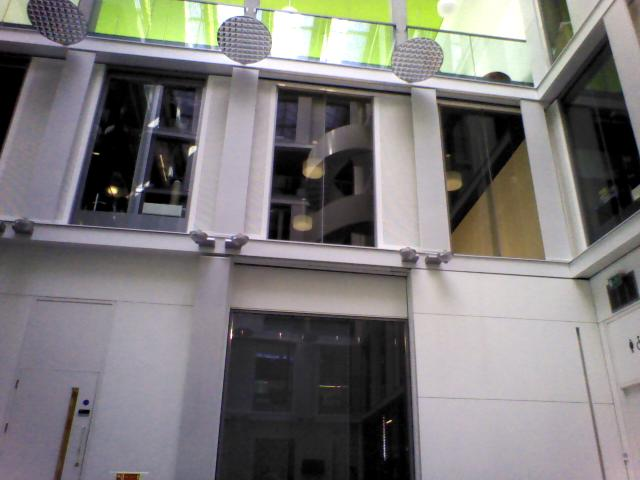
\includegraphics[scale=0.5]{../Drawings/datasetImages/dataset3_1.jpg}
\caption{A typical image from the first large hall dataset}
\label{fig:largeHall1}
\end{minipage}
\hspace{0.5cm}
\begin{minipage}[b]{0.5\linewidth}
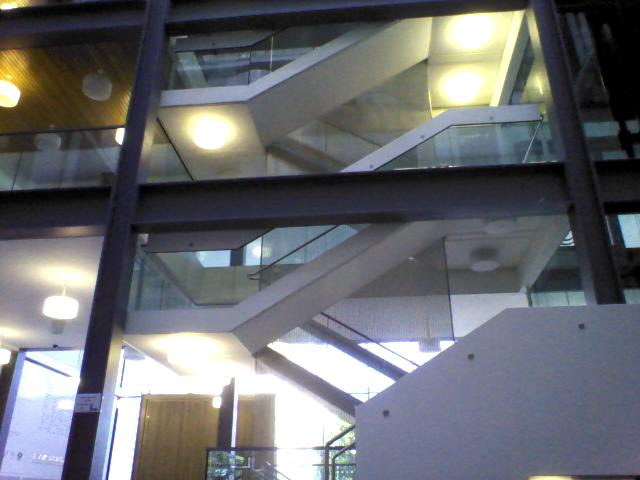
\includegraphics[scale=0.5]{../Drawings/datasetImages/dataset3_2.jpg}
\caption{A typical image from the second large hall dataset}
\label{fig:largeHall2}
\end{minipage}
\end{figure}

Again, all four of the feature extraction techniques have been tested on overlapping and non-overlapping images. In this case there are $210$ overlapping image pairs and $210$ non-overlapping image pairs. The ROC curves generated from this experiment are shown in \figref{fig:compareKnnOffice3} to \figref{fig:compareHammingConsistentOffice3} respectively. The statistics quantifying these ROC curves are shown in \tabref{tab:hallStatsKnn} and \tabref{tab:hallStatsHamming} respectively.\\

\begin{figure}[h!]
\begin{minipage}[b]{0.5\linewidth}
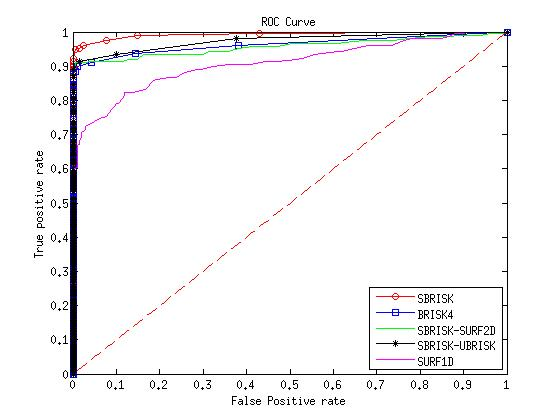
\includegraphics[scale=0.4]{../Drawings/dataset3_ROC_General_KNN.jpg}
\caption{A comparison of the ROC curves in the large hall environment using the MPS thresholds}
\label{fig:compareKnnOffice3}
\end{minipage}
\hspace{0.5cm}
\begin{minipage}[b]{0.5\linewidth}
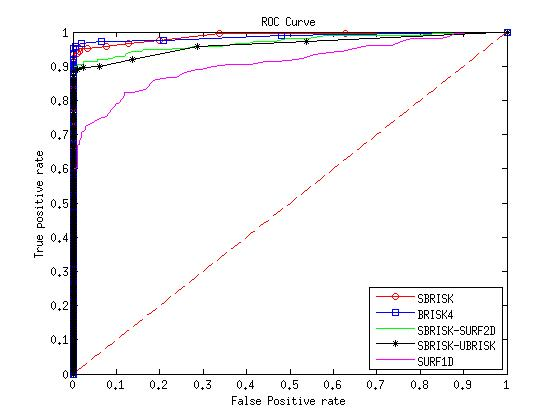
\includegraphics[scale=0.4]{../Drawings/dataset3_ROC_General_KNN_Consistent.jpg}
\caption{A comparison of the ROC curves in the large hall environment using the CPS thresholds}
\label{fig:compareKnnConsistentOffice3}
\end{minipage}
\begin{minipage}[b]{0.5\linewidth}
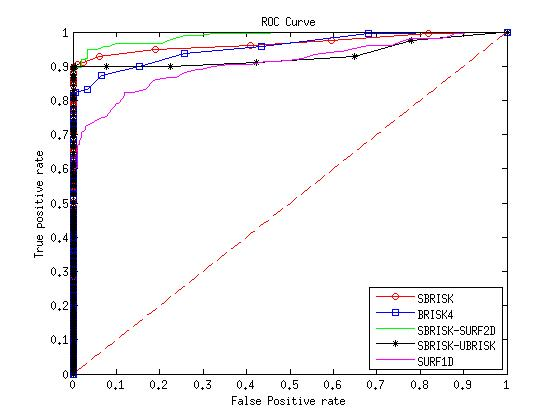
\includegraphics[scale=0.4]{../Drawings/dataset3_ROC_General_Hamming.jpg}
\caption{A comparison of the ROC curves in the large hall environment using the MPS Hamming/Euclidean distance thresholds}
\label{fig:compareHammingOffice3}
\end{minipage}
\hspace{0.5cm}
\begin{minipage}[b]{0.5\linewidth}
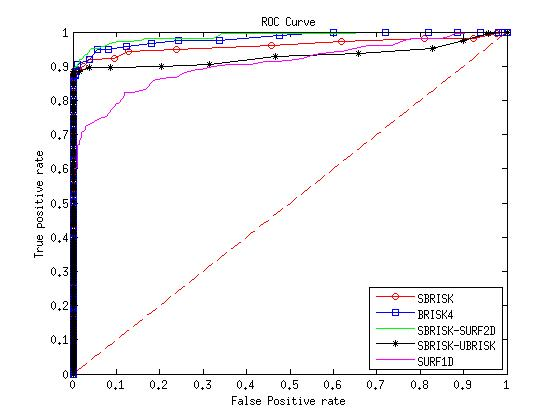
\includegraphics[scale=0.4]{../Drawings/dataset3_ROC_General_Hamming_Consistent.jpg}
\caption{A comparison of the ROC curves in the large hall environment using the CPS Hamming/Euclidean distance thresholds}
\label{fig:compareHammingConsistentOffice3}
\end{minipage}
\end{figure}

\begin{table}

\tiny
\caption{The AUC and performance statistics for the large hall environment
using 2-NN}


\begin{tabular}{|c|c|c|c|c|c|c|c|}
\hline 
\textbf{Method} & \textbf{Parameters} & \textbf{\% AUC} & \textbf{Detection(ms)} & \textbf{Extraction(ms)} & \textbf{Matching(ms)} & \textbf{Verification(ms)} & \textbf{Overall(ms)}\tabularnewline
\hline 
\hline 
BRISK0 & MPS & 99.263 & 4.0270 & 10.752 & 18.175 & 0.14700 & 37.513\tabularnewline
\hline 
BRISK4 & MPS & 96.444 & 15.664 & 9.6910 & 13.698 & 0.12600 & 43.645\tabularnewline
\hline 
BRISK0-SURF2D & MPS & 95.697 & 4.2080 & 22.242 & 4.2410 & 0.18800 & 35.389\tabularnewline
\hline 
\textbf{BRISK0-UBRISK} & \textbf{MPS} & \textbf{97.430} & \textbf{3.7010} & \textbf{3.8040} & \textbf{9.8490} & \textbf{0.10900} & \textbf{21.885}\tabularnewline
\hline 
BRISK0 & CPS & 98.798 & 5.4120 & 22.181 & 81.944 & 0.30600 & 114.365\tabularnewline
\hline 
BRISK4 & CPS & 98.703 & 28.349 & 23.880 & 83.456 & 0.29800 & 140.463\tabularnewline
\hline 
BRISK0-SURF2D & CPS & 97.024 & 5.4430 & 42.449 & 14.060 & 0.34900 & 66.809\tabularnewline
\hline 
\textbf{BRISK0-UBRISK} & \textbf{CPS} & 96.186 & 4.7870 & 7.2480 & 46.827 & 0.23200 & 63.541\tabularnewline
\hline 
\textbf{SURF 1D} & \textbf{Given} & \textbf{90.836} & \textbf{0.27300} & \textbf{0.16100} & \textbf{0.35100} & \textbf{0.044000} & \textbf{14.032}\tabularnewline
\hline 
\end{tabular}
\label{tab:hallStatsKnn}
\end{table}


\begin{table}
\caption{The AUC and performance statistics for the large hall environment
using Hamming/Euclidean distance}
\tiny
\begin{tabular}{|c|c|c|c|c|c|c|c|}
\hline 
\textbf{Method} & \textbf{Parameters} & \textbf{\% AUC} & \textbf{Detection(ms)} & \textbf{Extraction(ms)} & \textbf{Matching(ms)} & \textbf{Verification(ms)} & \textbf{Overall(ms)}\tabularnewline
\hline 
\hline 
BRISK0 & MPS & 96.739 & 3.2330 & 4.5650 & 2.3210 & 0.021000 & 14.642\tabularnewline
\hline 
BRISK4 & MPS & 95.516 & 10.115 & 3.9520 & 1.3410 & 0.017000 & 19.893\tabularnewline
\hline 
BRISK0-SURF2D & MPS & 98.803 & 3.4360 & 11.197 & 1.2600 & 0.039000 & 20.345\tabularnewline
\hline 
\textbf{BRISK0-UBRISK} & \textbf{MPS} & \textbf{93.150} & \textbf{3.2490} & \textbf{2.5160} & \textbf{2.6140} & \textbf{0.026000} & \textbf{12.824}\tabularnewline
\hline 
BRISK0 & CPS & 96.070 & 3.2680 & 4.7620 & 2.6180 & 0.028000 & 15.091\tabularnewline
\hline 
BRISK4 & CPS & 98.269 & 12.123 & 6.1390 & 4.3590 & 0.045000 & 27.164\tabularnewline
\hline 
BRISK0-SURF2D & CPS & 98.786 & 3.6030 & 13.475 & 1.7170 & 0.051000 & 23.414\tabularnewline
\hline 
BRISK0-UBRISK & CPS & 92.964 & 3.3030 & 2.5810 & 2.6180 & 0.030000 & 13.503\tabularnewline
\hline 
\textbf{SURF 1D} & \textbf{Given} & \textbf{90.836} & \textbf{0.27300} & \textbf{0.16100} & \textbf{0.35100} & \textbf{0.044000} & \textbf{14.032}\tabularnewline
\hline 
\end{tabular}
\label{tab:hallStatsHamming}
\end{table}
%\subsubsection{BRISK0}
%\label{sec:briskResults}
%
%\subsubsection{BRISK}
%\label{sec:brisk2dsurfResults}
%
%\subsubsection{BRISK0-SURF2D}
%\label{sec:brisk2dsurfResults}
%
%
%\subsubsection{BRISK0 - U-BRISK}
%\label{sec:BRISK0Results}
%
%
%\subsubsection{1DSURF}
%\label{sec:1dsurfResults}

Therefore, based on the above data, the BRISK0- U-BRISK algorithm using \textit{RadiusMatch} matching technique seems to produce the best performance and should therefore be implemented on the robot. Since it can perform image processing and feature extraction in approximately $11 ms$, it should be possible to use this method in real-time on the robot to perform the matching routine and ultimately help the robot disambiguate its position on the field.\\

\subsection{Matching Score Boundary}
\label{sec:matchingScoreBoundary}
In order to effectively utilise this method on the robot, a matching score boundary (MSB) needs to be determined. When matching two images, if the matching score is above the MSB, then the images are matched. If the matching score is below the MSB then the images are not matched. \\

The MSB needs to be defined such that no False Positives (FP) will be generated when matching two non-overlapping images. In order to implement this constraint, a threshold has been chosen on the ROC curve that produces the maximum amount of True Positive (TP) matches whilst still producing no FPs. Using the original Robocup dataset, a MSB of $0.13$ has been chosen which produces a TP rate of $0.38$ and a FP rate of $0$. This means that approximately $1$ out of every $2.5$ overlapping images will be classified as a TP. This is acceptable performance since the Nao's camera takes $30$ frames per second according to Aldebaran's documentation and therefore the robot will process a large number of frames in a short period of time enabling it to ultimately match two images if they are indeed a match.\\




\subsection{Lighting Variation}
\label{sec:lighting}
An important consideration that has to be taken into account is how well the feature extraction algorithm performs under conditions of varying illumination. This is important because Robocup venues change every year and the illumination may not be uniform. In order to determine how well BRISK0-U-BRISK performs in these conditions, three scenarios were created with varying lighting conditions. All of these scenarios were created in the Robocup test environment, detailed in \secref{sec:datasets}.\\ 

For each scenario $i$ four image datasets were generated as in \secref{sec:datasets}. These include  two datasets of images behind the player's goal namely, \textit{$PG Left_{i}$} and \textit{$PG Right_i$} as well as two datasets behind the opponent's goal, namely \textit{$OG Left_i$} and \textit{$OG Right_i$} respectively. Each image dataset contains $15$ images. All of the images in each dataset were taken at the same scale since only the performance under varying illumination is being tested in this experiment.\\ 

The lighting setup in the Robocup test environment is as follows. The environment contains a main set of lights that are responsible for providing the general lighting in the room. In addition to these lights are a set of two fluorescent lights that lie adjacent to one another on the ceiling. Each fluorescent light stretches the length room and is responsible for adding additional lighting to the scene. \\

Scenario $1$ involves switching off only a single fluorescent light located on the ceiling. Typical images from each dataset generated in this scenario are shown in \figref{fig:leftmgleft} to \figref{fig:leftogright} respectively. Scenario $2$ involves turning off only a single fluorescent light located on the ceiling as well as the main set of lights. Typical images from these datasets are shown in \figref{fig:rightmgleft} to \figref{fig:rightogright} respectively. Scenario $3$ involves turning off both fluorescent lights, leaving only the main lighting in the environment. Typical images from these datasets are shown in \figref{fig:bothmgleft} to \figref{fig:bothogright} respectively. \\

Each of the datasets from the three scenarios have been matched with the original corresponding Robocup datasets detailed in \secref{sec:datasets}. This means that, for example, \textit{$PG Left_1$} from scenario $1$ will be matched to \textit{PG Left} and so on. These datasets are being compared in order to determine whether or not the BRISK0 - U-BRISK algorithm is robust to variations in illumination. The datasets have been matched as shown in \tabref{tab:datasetLighting} to produce $1260$ pairs of overlapping images and $4536$ pairs of non-overlapping images under varying lighting conditions.\\


\begin{figure}
\begin{minipage}[b]{0.5\linewidth}
\includegraphics[scale=0.3]{../Drawings/lighting/leftLight/1.jpg}
\caption{The area behind the player's goal to the left}
\label{fig:leftmgleft}
\end{minipage}
\hspace{0.5cm}
\begin{minipage}[b]{0.5\linewidth}
\includegraphics[scale=0.3]{../Drawings/lighting/leftLight/2.jpg}
\caption{The area behind the player's goal to the right}
\label{fig:leftmgright}
\end{minipage}
\begin{minipage}[b]{0.5\linewidth}
\includegraphics[scale=0.3]{../Drawings/lighting/leftLight/3.jpg}
\caption{The area behind the opponent's goal to the left}
\label{fig:leftogleft}
\end{minipage}
\hspace{0.5cm}
\begin{minipage}[b]{0.5\linewidth}
\includegraphics[scale=0.3]{../Drawings/lighting/leftLight/4.jpg}
\caption{The area behind the opponents goal to the right}
\label{fig:leftogright}
\end{minipage}
\caption{Typical images from the first illumination scenario where only a single light is turned off}
\end{figure}



\begin{figure}
\begin{minipage}[b]{0.5\linewidth}
\includegraphics[scale=0.3]{../Drawings/lighting/rightLight/1.jpg}
\caption{The area behind the player's goal to the left}
\label{fig:rightmgleft}
\end{minipage}
\hspace{0.5cm}
\begin{minipage}[b]{0.5\linewidth}
\includegraphics[scale=0.3]{../Drawings/lighting/rightLight/2.jpg}
\caption{The area behind the player's goal to the right}
\label{fig:rightmgright}
\end{minipage}
\begin{minipage}[b]{0.5\linewidth}
\includegraphics[scale=0.3]{../Drawings/lighting/rightLight/3.jpg}
\caption{The area behind the opponent's goal to the left}
\label{fig:rightogleft}
\end{minipage}
\hspace{0.5cm}
\begin{minipage}[b]{0.5\linewidth}
\includegraphics[scale=0.3]{../Drawings/lighting/rightLight/4.jpg}
\caption{The area behind the opponents goal to the right}
\label{fig:rightogright}
\end{minipage}
\caption{Typical images from the second illumination scenario where a single fluorescent light as well as the main lighting is turned off.}
\end{figure}



\begin{figure}
\begin{minipage}[b]{0.5\linewidth}
\includegraphics[scale=0.3]{../Drawings/lighting/bothLights/1.jpg}
\caption{The area behind the player's goal to the left}
\label{fig:bothmgleft}
\end{minipage}
\hspace{0.5cm}
\begin{minipage}[b]{0.5\linewidth}
\includegraphics[scale=0.3]{../Drawings/lighting/bothLights/2.jpg}
\caption{The area behind the player's goal to the right}
\label{fig:bothmgright}
\end{minipage}
\begin{minipage}[b]{0.5\linewidth}
\includegraphics[scale=0.3]{../Drawings/lighting/bothLights/3.jpg}
\caption{The area behind the opponent's goal to the left}
\label{fig:bothogleft}
\end{minipage}
\hspace{0.5cm}
\begin{minipage}[b]{0.5\linewidth}
\includegraphics[scale=0.3]{../Drawings/lighting/bothLights/4.jpg}
\caption{The area behind the opponents goal to the right}
\label{fig:bothogright}
\end{minipage}
\caption{Typical images from the third illumination scenario where a both fluorescent lights are turned off.}
\end{figure}
\begin{table}
\caption{The datasets that have been compared under varying lighting conditions
to the original Robocup datasets}


\begin{tabular}{|c|c|c|c|}
\hline 
\textbf{Dataset} & \textbf{Scenario Dataset} & \textbf{Overlapping Image Pairs} & \textbf{Non-overlapping Image pairs}\tabularnewline
\hline 
\hline 
 &  &  & \tabularnewline
\hline 
\textbf{Original Dataset} & Scenario 1 (Left fluorescent Light Off) & 420 & 1512\tabularnewline
\hline 
\textbf{Original Dataset} & Scenario 2 (Right fluorescent light and Main Lights off) & 420 & 1512\tabularnewline
\hline 
\textbf{Original Dataset} & Scenario 3 (Both fluorescent Lights off) & 420 & 1512\tabularnewline
\hline 
 &  & 1260 & 4536\tabularnewline
\hline 
\end{tabular}
\label{tab:datasetLighting}
\end{table}

ROC curves have been generated for each scenario and are shown in \figref{fig:rocLighting}. The ROC curve with the poorest performance is generated from the third scenario. This scenario corresponds to the lowest illumination since both the fluorescent lights are turned off. It is therefore expected that this scenario would produce the worst performance relative to the other two. The marginally best performing datasets are from scenario two where a fluorescent light and the main lights are turned off. \\

The statistics corresponding to the ROC curves are tabulated in \tabref{tab:lightingStats}. It should be noted that AUC values of over $90\%$ have been recorded indicating a high level of matching performance. \\


\begin{figure}[h!] 
  \centering
    \includegraphics[width=0.5\textwidth]{../Drawings/lighting/ROC_Lighting.jpg}
    \caption{The ROC curve showing the performance of the BRISK0 - U-BRISK algorithm under varying lighting conditions}
    \label{fig:rocLighting}
\end{figure}

\begin{table}
\caption{The statistics for the matching performance under varying lighting conditions}
\begin{tabular}{|c|c|c|c|c|c|c|}
\hline 
Scenario & \% AUC & Detection(ms) & Extraction(ms) & Matching(ms) & Verification(ms) & Overall Time (ms)\tabularnewline
\hline 
\hline 
1 & 95.315 & 2.9820 & 1.7030 & 0.23200 & 0.0080000 & 8.7850\tabularnewline
\hline 
2 & 96.957 & 2.9530 & 1.7110 & 0.22900 & 0.0070000 & 8.7640\tabularnewline
\hline 
3 & 93.217 & 3.0400 & 1.9480 & 0.28300 & 0.0080000 & 9.3090\tabularnewline
\hline 
\end{tabular}
\label{tab:lightingStats}
\end{table}

\subsection{Localisation Performance}
\label{sec:localisationPerformance}







\section{Conclusion}
\label{sec:conclusion}

\bibliographystyle{witseie}
\bibliography{bibliography}
% \newpage
%\onecolumn
%\appendix
%\setcounter{table}{0}
%\setcounter{figure}{0}
%\setcounter{subsection}{0}
%\makeatletter \renewcommand{\thefigure}{A.\@arabic\c@figure} \renewcommand{\thetable}{A.\@arabic\c@table} \renewcommand{\thesection}{A.\@arabic\c@section} \makeatother
%\section*{APPENDIX A}
%
%\section{Control Program}
%Add the matlab code to this file...
%\lstinputlisting{codeSnippets.cpp}
 
\end{document}

